\documentclass[10pt,twoside]{book}
\usepackage[paperwidth=6in,paperheight=9in,
inner=0.95in,outer=0.6in,top=0.75in,bottom=0.85in,
bindingoffset=0.12in]{geometry}
\pdfpagewidth=6in
\pdfpageheight=9in

% Use system fonts (XeLaTeX/LuaLaTeX)
\usepackage{fontspec}
\usepackage{titlesec}
\usepackage{imakeidx}
\makeindex[intoc,columns=2]
\setmainfont{InfoOTDisp}
\setmonofont[
    Scale=1.0
]{Courier New}
\newfontfamily\headingfont{Eurostile W01}
\newfontfamily\chapterfont{Eurostile Extd}


\titleformat{\section}
  {\headingfont\Large\bfseries}
  {\thesection}{1em}{}

\titleformat{\subsection}
  {\headingfont\large\bfseries}
  {\thesubsection}{1em}{}

\titleformat{\subsubsection}
  {\headingfont\normalsize\bfseries}
  {\thesubsubsection}{1em}{}

% Microtypography for tighter, book-like setting
\usepackage{microtype}
\linespread{0.98}

\usepackage{seqsplit}
%----------------------------------------------------------------------------------------
%	Titles and Headings Code
%----------------------------------------------------------------------------------------
\usepackage{titlesec}
\titleformat{\chapter}[hang]{\chapterfont\large}{\thechapter}{1em}{}
\titlespacing*{\chapter}{0pt}{-10pt}{10pt}

% Simple headers/footers
\usepackage{fancyhdr}
\setlength{\headheight}{21pt} % at least 20.68404pt; 21pt is safe
\pagestyle{fancy}
\fancyhf{}
\renewcommand{\headrulewidth}{0pt}
\fancyhead[LE,RO]{\thepage}
\fancyhead[RE,LO]{\small\itshape \leftmark}

\usepackage{float}
%---------- ENDNOTES -----------------
% Endnotes: inline [n], printed later
\usepackage{endnotes}
\renewcommand{\enoteheading}{} % suppress heading

% Mark in the text: [n]
\renewcommand{\enoteformat}{\textnormal{[\theenmark]}}

% If you have an "endnotes printed later" style, this helps ensure correct marks
\makeatletter
\renewcommand{\@endnotemark}{\textnormal{[\theenmark]}}
\makeatother

% Print endnotes (call once per chapter, at end)
\newcommand{\printchapterendnotes}{%
  \cleardoublepage
  \begingroup
    \chapter*{Endnotes}%
    \addcontentsline{toc}{chapter}{Endnotes}%
    \theendnotes
  \endgroup
  \setcounter{endnote}{0}%
}

%--------- Figures ----------------
\usepackage{rotating}
\usepackage{graphicx}
\usepackage[section]{placeins}
%--------- Math ----------------
\usepackage{amsmath}


\usepackage[toc,nonumberlist,nopostdot]{glossaries}
\makeglossaries
% Glossary entries — use \gls{label} or \Gls{label} in text.
% Acronyms — use \acrfull{label}, \acrshort{label}, or \acrlong{label} in text.

%----------------------------------------------------------------------------------------
%	Terms
%----------------------------------------------------------------------------------------
\newglossaryentry{amnesiac}{
    name=amnesiac,
    description={OED:  (1913-) "One who is afflicted with amnesia." \footnote{  
    “Amnesiac, N.” Oxford English Dictionary, Oxford UP, December 2024, \url{https://doi.org/10.1093/OED/9207200444}.}}
}



\newglossaryentry{bsd}{
    name=BSD,
    description={Berkeley Software Distribution, a Unix-derived operating system and its variants (FreeBSD, OpenBSD, NetBSD)}
}

\newglossaryentry{coding}{
    name=coding,
    description={
    The OED described coding as (1946-)"3.  Computing. The conversion of information into code usable by a computer or other machine; the writing or editing of code for a computer program, application, etc. Also: computer code."
    \footnote{
    “Coding, N., Sense 3.” Oxford English Dictionary, Oxford UP, June 2025, \url{https://doi.org/10.1093/OED/4701717734}.
    }
    }
}


\newglossaryentry{configuration}{
    name=configuration,
    description={The OED describes configuration as (1962) "8. Computing. The way the constituent parts of a computer system are chosen or interconnected in order to suit it for a particular task or use; the units or devices required for this." 
    \footnote{
    “Configuration, N., Sense 8.” Oxford English Dictionary, Oxford UP, June 2026, \url{https://doi.org/10.1093/OED/1065280211}.}
    }
}


\newglossaryentry{immutable system}{
    name=immutable system,
    description={
    The OED describes immuatable as (1621) "1.b.  technical. Not subject to variation in different cases; invariable: used e.g. of markings which are the same in all the individuals of a species."  
    \footnote{“Immutable, Adj., Sense 1.b.” Oxford English Dictionary, Oxford UP, December 2025, \url{https://doi.org/10.1093/OED/1176087402}.}  An immutable system is one that cannot be changed.  In these computing systems, the intent of using an immutable system is to allow an operator to restore a system to its original state by power cycling it.
    }
}

\newglossaryentry{kernel}{
    name=kernel,
    description={The core component of an operating system that manages hardware resources and provides services to user-space programs}
}

\newglossaryentry{jail}{
    name=jail,
    description={A FreeBSD OS-level virtualisation mechanism that partitions the operating system into isolated environments}
}

\newglossaryentry{port}{
    name=port,
    description={A directory in the FreeBSD Ports Collection containing the files needed to automatically compile and install a third-party application}
}

\newglossaryentry{zfs}{
    name=ZFS,
    description={A file system used in FreeBSD adapted from Oracle.}
}

\newglossaryentry{poudriere}{
    name=Poudriere,
    description={Named after the French word for ``powderkeg,'' Poudriere is a package building program that will custom-compile programs from ports and configuration files.  A FreeBSD operator can then use their own tailored programs built to specifications while obtaining updates from the ports tree.}
}

\newglossaryentry{}{
    name=,
    description={}
}





%----------------------------------------------------------------------------------------
%	Acronyms
%----------------------------------------------------------------------------------------

\newacronym{cissp}{CISSP}{Certified Information Systems Security Professional}
\newacronym{csslp}{CSSLP}{Certified Secure Software Lifecycle Professional}
\newacronym{ccsp}{CCSP}{Certified Cloud Security Professional}
\newacronym{os}{OS}{Operating System}
\newacronym{ssh}{SSH}{Secure Shell}
\newacronym{tls}{TLS}{Transport Layer Security}
\newacronym{acl}{ACL}{Access Control List}
\newacronym{ids}{IDS}{Intrusion Detection System}
\newacronym{ips}{IPS}{Intrusion Prevention System}
\newacronym{vpn}{VPN}{Virtual Private Network}
\newacronym{ram}{RAM}{Random Access Memory}
\newacronym{vnet}{VNET}{Virtual Network}
\newacronym{gb}{GB}{GigaBytes}
\newacronym{dvd}{DVD}{Digital Video Disc}
\newacronym{rw}{RW}{Read Write}
\newacronym{lto}{LTO}{Linear Tape Open}
\newacronym{ssd}{SSD}{Solid State Drive}
\newacronym{sas}{SAS}{Serial Attached SCSI}
\newacronym{sata}{SATA}{Serial AT Attachment}
\newacronym{nic}{NIC}{Network Interface Card}
\newacronym{gpu}{GPU}{Graphics Processing Unit}
\newacronym{nist}{NIST}{National Institute of Standards and Technology}


\usepackage[colorlinks=true, linkcolor=black, urlcolor=blue, citecolor=black]{hyperref}

\usepackage{xurl}
% Paragraph and list compactness
\setlength{\parindent}{1.5em}
\setlength{\parskip}{0pt}
\usepackage{enumitem}
\setlist{nosep}

% Figure captions compact
\usepackage[font=small,labelfont=bf]{caption}
\renewcommand{\figurename}{Fig.}

% Code style approximating K&R (monospaced, compact)
\usepackage{xcolor}
\usepackage{listings}
\usepackage{amsmath}
\usepackage{booktabs}
\usepackage{array} % optional for >{\raggedright\arraybackslash}
\lstset{
  basicstyle=\ttfamily\small,
  keywordstyle=\bfseries,
  commentstyle=\itshape\color{gray},
  numbers=left, numberstyle=\tiny\color{gray}, numbersep=6pt,
  stepnumber=5,
  frame=none, xleftmargin=2em,
  tabsize=4,  showstringspaces=false,
  columns=fullflexible,
    breaklines=true,
  breakatwhitespace=false,
  keepspaces=true
}
\lstdefinelanguage{KRC}{language=C}


% makecell for table header adjustments
\usepackage{makecell}
\setcellgapes{2pt}
\makegapedcells
%\renewcommand{\arraystretch}{1.15}




% Title page simple
\title{{\chapterfont \index{coding}\Gls{coding} and \Gls{configuration} \\for Secure Systems in BSDs}}
\author{John O\string'Keefe-Odom}
\date{}

\begin{document}

\newpage
\thispagestyle{empty}   % no page number or header
\vspace*{\fill}         % push text to vertical center
\begin{center}
  \itshape              % italics are traditional
  For the nameless victims I saw at work one day.\\We are coming to the rescue of our memory of your worst days.\\We know that cybercrime became a crime when it hurt you.
\end{center}
\vspace{\fill}
\newpage

\maketitle
\frontmatter
\tableofcontents

%----------------------------------------------------------------------------------------
%	Author
%----------------------------------------------------------------------------------------
\chapter*{Author}
\addcontentsline{toc}{chapter}{Author}

John O\string'Keefe-Odom received a Master of Liberal Arts (ALM) in Extension Studies in the field of Cybersecurity from Harvard Univerisity,\index{University!Harvard!Extension School} Harvard University Extension School, in 2026.  He received an AAS in Web Programming from\index{Chattanooga}\index{Community College!Chattanooga State} Chattanooga State Community College in 2013.  He received a BA in English:  Writing from the \index{University!of Tennessee!at Chatttanooga}University of Tennessee at Chattanooga \index{Chattanooga}in 2001.  He holds various technical certifications in cybersecurity including:  \gls{cissp}, \gls{csslp}, \gls{ccsp}, SecurityX, PenTest+, CySA+, Security+, and Linux+.  He has worked as a senior application security engineer and software engineer for various companies for over ten years.  

%----------------------------------------------------------------------------------------
%	Foreword
%----------------------------------------------------------------------------------------
\chapter*{Preface}
\addcontentsline{toc}{chapter}{Preface}

Your preface text goes here...

%----------------------------------------------------------------------------------------
%	Acknowledgements
%----------------------------------------------------------------------------------------
\chapter*{Acknowledgements}
\addcontentsline{toc}{chapter}{Acknowledgements}

As a web programmer, I make a hundred mistakes a day. If I make less than that, I'm behind.  When it comes to computing, mine has been a path of hammering.  I'm the type of person who will hammer and hammer and hammer away at the problem until I eventually break through.  So, I can't promise you a flawless path to success, but I can suggest that we will learn something from this journey.

The mistakes and omissions which follow are entirely mine.  I would like to thank some people for their help along the way.

If I had not found our local hacking group DC423, then I might not have sustained a professional interest in cybersecurity so successfully.  If I had not attended many \index{B-Sides}B-Sides security conferences around the Southeastern US, then I might not have realized how grand and stimulating the community of hackers really is.  

I had many influential professors along the way.  I fell into the right crowd of instructors at \index{Community College!Chattanooga State}Chattanooga State Community College with Leigh MacGregor, Mrs. Peacock, and host of others whose names I cannot recall.  Doctors Kizza, Dumas, Kandah, and especially Li Yang from the \index{University!of Tennessee!at Chatttanooga}University of Tennessee at Chattanooga built a base that prepared me for later challenges in Computer Science.  Ken Smith, MFA, was my mentor for writing at UTC.  I have many fond memories of the faculty during my undergraduate years there as an English major.  I studied under heroes of the intellect like Doctors Richards, Noe, Rehyansky, Ware, and many others.  \index{University!Harvard!Extension School}At Harvard Extension School, I'm sure I pissed off almost every TA and instructor who had the misery of grading my work.  For them, I am grateful.  Many thanks to my  professors at Harvard:  Len Evanchik, Daniel Garrie, David Cass, Derek Brink, Ramesh Nagappan, Joseph Ficara, Minlan Yu, David Arias, Eddie Kohler, David Malan, and Bruce Huang.  And, of course, an extra special thanks to the professor for whom I was her "most challenging student," Heather Hinton. 

With our chosen style of citations, we tried to provide references that would withstand common lab use and academic rigor.  We provided in-chapter sections for convenient references to books, man pages, and websites.  We also continued with inline footnoting for chapter endnotes; we especially noted various computer commands and technologies since they are fundamentally derivative works upon which we depend.  This made for a lot of references and some duplicity.  We have cited generously.

We decided to set a previous book in fonts by Erik Spiekermann after seeing ``Helvetica'' by Gary Hustwit (2007). We carried that through here.  InfoOTDisp-Book is copyrighted by Ole Schaefer and Erik Spiekermann; it is published by FSI Fonts und Software GmbH.  Eurostile Extended Regular and Eurostile W01 Regular are copyrighted 2006 and 2010 by URW Design and Development.  

For typesetting and formatting, we chose LaTex.  We repeatedly consulted various AI and Internet sources for coding the document which generated the paper.  For bibliographic formatting, we frequently used MyBib. \endnote{Mybib. “MyBib Bibliography Generator.” MyBib.Com, 13 July 2018, \url{https://www.mybib.com}. Accessed 12 July 2026.}
  
\printchapterendnotes
%----------------------------------------------------------------------------------------
%	Introduction
%----------------------------------------------------------------------------------------
\chapter*{Introduction}
\addcontentsline{toc}{chapter}{Introduction}

Your introduction text goes here...

\printchapterendnotes
\mainmatter


%Chapter 1: Introduction
%Background and Content
%Problem Statement
%Project Objectives
%Scope of Work
%Variables
%Assumptions, Risks, and Limitations
%Significance of the Project

%Chapter 2: Literature Review
%Overview of Existing Solutions or Approaches
%Comparisons of Technologies or Frameworks
%Gaps in the Literature

%Chapter 3: Methodology
%Technical Research Questions
%System Architecture / Design
%Implementation Plan
%Testing and Evaluation Strategy
%Data Procurement and Logging
%Ethical and Legal Considerations
%Limitations
%Changes To Initial Project Goals

%Chapter 4: Analysis
%Data Sources
%Risk Registry
%Protocols and Standard in the Field
%Mobile Geotagging
%RED Application
%Accessing RED
%Data Governance
%Data Visualization

%Chapter 5: Findings
%Impact on Industry
%Use of Sequential Numbers
%Changes in Governance
%Legislative Impact
%Reduce Legacy Impact
%Use Cases for Adoption of RED
%Future of the RED Project
%Enhance RED Data 

%\begin{figure}[H]
%  \centering
%  \caption{}
%  \label{fig:}
%\end{figure}
%----------------------------------------------------------------------------------------
% CHAPTER
%----------------------------------------------------------------------------------------
\chapter{Anecdotes on the Journey}

As I've encountered different problems related to computer systems in my life, I have noticed that sometimes other people don't react the way I might expect.  Sometimes people are supportive of finding and treating vulnerabilities.  Other times, people have told me directly that they didn't want any problems mentioned for fear that admitting there was a problem would make their system look weak.  Still other people have sometimes reacted in ways that were so self-centered that their reactions seemed foolish, almost comical.  Having seen some of these reactions, I noticed that our values and judgements about actors and victimization play a big role in how we might react to finding out we are the victims of attacks on computer systems.  I would like for us to think a little about how we might choose to value ourselves, the people working around us, and others affected by malfeasance on the web.  To that end, I would like to tell you a few small tales about my life and computers. 

\section{Computers and Insects} 

When I was a small boy, we lived in New Orleans.  In my part of the city, there was a large, open drainage canal.  This canal had steep sides covered with grass and weeds.  Most of the time the water was low in the canal.  Brown water snaked through the basin of the canal.  Sometimes there would be a muddy shopping cart in the weeds.  One time I saw an old man fishing for a turtle in the canal.  He used a big hook and a piece of meat.  He caught one large snapping turtle.  With a taut line, he pulled the turtle from the waters of the canal.  The snapping turtle was dripping with tan mud.  Its shell seemed as large as the man's torso.  He lifted it up and dropped it in a burlap sack.  He quickly gathered the top corners and held the bag shut with his fist. 

I had been picking blackberries in the brambles of the canal.  As I put my blackberries in my plastic margarine tub, I asked the man why he was fishing for the turtle.  He told me he was going to eat the turtle.  He would make turtle soup.   

I often saw rat traps tied with strings to trees in the canal.  Some people had houses along one side of the canal.  Along the edge of their backyards, they tied rat traps to tree trunks or metal fence posts.  These rat traps were like mouse traps, but much larger. Nobody ever bothered to put bait in them.  I lived in an apartment complex on the other side.  Every day I would walk to and from school with other kids from my neighborhood.  Every day, we would pass that canal. 

One day, near 1979, a computer programmer came to my school.  Our teacher gathered us in the library.  We sat in a circle on the floor, cross-legged, "Indian style."  The programmer came in, pushing his cart.  Taking up the whole top of the cart was the computer; it was a big gray box with a keyboard and a built-in monitor.  Underneath, on the shelf, was another set of boxes.  One of them was an eight-inch floppy disk drive.   

The programmer told us about computers.  Looking back, I realize that I forgot everything he said. He had shown us about files and the parts of the computer.  Then, there, on the computer screen, I saw something fascinating:  my first look at a video game.  It was Pac-Man in black-and-white.  There were no colors on the screen. 

One day I was walking home from school with the other kids.  Because I was little, I had to walk to and from school with one of the big kids, Jeanie.  She would watch out for me and make sure I went the right way.   

As we passed the canal every day, there was a little draw, like a V or little valley, going from the curb of the street down to where there was a big pipe.  The canal went under the road in this a big concrete pipe.  Some of the big kids would go down to the rim of the pipe and stand on its edge.  I was too little for that yet.  Instead, like most of the kids, I would run and jump across the little V at the top.  It was only a few steps, a few feet, but it felt like a big adventure when I made it across. 

I was having fun and feeling great in the sun, fresh out of school, I decided to run.  I ran, and I jumped.  I tried to get across the little V, but I didn't make it.  I tumbled and fell into the dirt on the wall of the little valley that went down to the big pipe. 

I jumped. I stumbled, and I fell.  I landed in a big ant pile.  There, on the far side of the V was a big ant pile.  It was about three feet around.  The puffy grains of cultivated dirt stood knee high to a man.  The ant pile was filled with hundreds of ants.  Before I knew it, before I felt myself really fall, I was swarmed and covered with ants! 

They were biting me! I forgot about the big canal.  I scrambled up the dirt.  They were all over me!  Hundreds of ants!  Ants on my back. Ants on my legs.  Ants on my arms, in my hair and on my head.  I did what any kid would do:  I screamed and cried and ran.  I ran as fast as I could.  I ran across the grass into the apartment complex.  I ran down the streets to my home.  I ran as fast as I could. 

I cried for my Mutti and told her about the ants.  She put me in a cold bath.  A little while later Jeanie came by with my book bag.  I had dropped it when I ran home.  She had rescued it. She told my Mutti about the ants.  I still remember my mom saying that she knew.  She had been glad Jeanie had checked up on me when I got home. 

It gets hot in New Orleans.  I still remember having to wear a white, long-sleeved shirt to school.  It was so hot and humid.  I felt sweaty, having to wear the long-sleeved dress shirt.  Often in New Orleans, I would play in shorts and a short-sleeved shirt.  I would often run barefoot and get a suntan.  But, thanks to the ants, I had to go to school in a long-sleeved shirt.  I was so covered with ant bites that it looked like I had the chicken pox.  I had to wear the long-sleeved shirt to keep from scratching. 

The next time a computer came into my life was some years later.  Now, my friends, and later I, had an Atari 2600.  Today I would look upon this as a computer, but back then, to me, it was "a video game."  Also, I had seen some other computers.  I had an old friend whose family was more rich; they had an IBM PCjr.  I saw Apple IIe's at school.  I had even attended a week-long summer camp at junior high.  I remember typing in my programs in BASIC.  I somehow had a book that I had gotten about computer programs.  It was about typing in programs to make a computer game.  I don't remember the title.  I don't have the book anymore.  I don't know what language it was written in.  However, the book was about adventures.  That's what I wanted:  computers and games and adventures.  I never did get many of those programs to work. 

I also remember my friend next to me, Eddie, typing in a program in another way.  I asked Eddie what it was.  He said it was C.  C!  The teacher said C was advanced.  He didn't want the rest of us to be trying to type programs in C, if we didn't know what we were doing.  It was okay for Eddie to try, because he was advanced.  The next week, there was another week of computer camp.  I didn't go because I thought it was for the advanced kids.   

The computers we used at school and saw around us:  they were expensive computers.  They cost thousands of dollars.  It was clear to me that I shouldn't even ask for one because there was no way we'd be able to buy one of those.  Yet, somehow, I ran across an ad in a magazine for a Commodore 64.  It was \$200. 

Now, that was a lot of money back then, too.  It was a bare-bones system.  I would still need some more components.  But, it was \$200.   

A friend of mine, Donald, had proudly told me at school how he had a job and made money mowing lawns and raking leaves.  That sounded pretty good to me:  making money.  I was mildly interested in lawn care.  Most of all, I knew I could do it.  I could push the lawnmower.  My dad made me mow the lawn.  I could earn some money.  I canvassed the neighborhood.  Some people said no.  Some people said they mowed their own lawn.  I didn't want to go too far up the street into Donald's territory.  I found one customer:  the man across the street. 

I mowed the lawn for \$20 a pop.  I was the worst employee you ever saw.  Frequently, I would just quit working.  It would be hot, and the Zoysia grass would be thick and wet.  It would clog up my lawnmower because I would wait too long to go back and mow again.  I would cut one rectangular patch in the thick part of the front yard.  It would get hot, and I would leave to cool off.  I would come back eventually and start mowing again.   

One day, I was bopping along, mowing real great, dreaming of imaginary greatness.  I had a good rhythm going. I was getting close to finishing at the end.  I bumped up against that big old Magnolia tree Mister Warner had in his yard.  Somewhere right around there, I hit a yellow jacket nest. 

I don't know if you've ever hit a yellow jacket nest with a lawnmower, but I want to tell you:  those yellow jackets were angry.  They do not want to be disturbed.  All they want to do is eat fruit, rotten insects, and sleep in their enormous, maze-like hell of an underground yellow jacket nest.   

I remember that I felt them buzzing around me and swarming.  I felt some heat on my arm, and looked down and saw one stinging.  I can still remember seeing one stuck in the skin of my arm, trying to pull away, as it stung me.   

This time, I was older.  I was more mature.  I was experienced.  When it came to stings, I was advanced.  I didn't just cry when I ran home.  I ran home aggressively. 

I started getting undressed outside.  I remember I stripped off my pants in the kitchen.  Insects were still buzzing in the legs of my jeans.  I swatted at them. I ran and got in a cold tub.  I still remember brushing at my arms and legs in the cold water.  I felt a few stingers come out.  The stings burned and throbbed and grew red.  I had a little over \$200.  I had been mowing all summer. 

As I scrounged over my hoarded money, it turned out that I had just enough to get the computer and a TV set.  I remember feeling stunned as my mother asked me if I had enough for tax.  Tax! What tax, I said.  Sales tax, they said.  How much was that, I asked in a daze.  Somehow, they must have saved me, because I came home with a computer and a black-and-white TV set to use as a monitor.   

It was a Commodore 64.  I would type the programs in.   It came with a manual.  I had learned a little BASIC in school.  Trouble was, every time I would turn the computer off, it would forget the programs.  You see, RAM is a volatile form of memory.  Without electricity constantly charging that type of memory, it would forget.  There was ROM in the computer, and in cartridges for games, but what was needed was a more persistent local storage.  I needed a tape drive.   

I had to go back and mow some more lawns.  I did go back.  I did mow some more lawns. Mister Warner did pay me, even though I was the worst employee ever.  He did help me to realize that there were jobs out there.  Yet, once I got that tape drive, I don't think I ever went back.  Soon we moved away, and I was on to the next adventure:  high school. 

After high school, I got my first chance at a real job:  joining the Army.  Now, at the time, I was only seventeen.  I remember telling my mom and dad, The recruiters said that since I was under age, you would have to sign for me.  I thought that would wrap up that effort.  Instead, my parents said, Where do I sign?  Next thing I knew, I was here and away to Basic Training.   

I learned how to work in Basic Training.  I put forth effort.  I felt like I was under a lot of stress, with no way to escape, for the first time in my life.  I learned how to work and get along with people I might not otherwise be around.  After Basic, I went on to radio school.  I became a RATT operator, radio automatic teletype.  I went to jump school.  I spent my enlistment jumping out of planes and operating radios.  It was a great job for a young man to have. 

This job was where I really learned about computers and telecommunications.  The Army made us do everything to send a message.  We began by learning to type on a 1949 teletype.  We learned how to generate our own electricity, and we learned how to hookup systems to commercial power if it was available.  We were taught to construct our own antennas, raise our own 50-foot antenna towers.  We used one-time pads, hardware and software encryption techniques.  We used punched paper tape, Bell Labs modems with oscilloscopes, teleprinters and shortwave radios.  We used encrypted, wireless networking systems back before the Internet became popular among the public. 

One day I was on the job during Operation Desert Shield in Saudi Arabia.  I had had a long day.  I had been up for most of the day.  I had worked the night shift.  I was about to go to bed when Sergeant D. told me, You have latrine detail.  Back then, we used burnout latrines.  So, what this means was that we would drag the cans of sewage out of the latrine hut, and burn off the sewage that had pooled inside.  To do this, you would use a five gallon can of diesel fuel; pour that into the can.  Then you would pour some unleaded gasoline into the can.  It would look pink over the yellowish diesel.  Immediately, a thick curtain of vapors would rise from the can.  With the cans loaded with fuel, we would get back some feet, crouch down, and strike and throw a match towards the curtain of gasoline vapor.  Whump!  The cans would catch flame.  One by one, we would set them on fire this way.   

Burning sewage takes hours.  What happens is that the burning unleaded gasoline ("MOGAS," we called it in the Army) will begin to heat up and boil the diesel.  Once the diesel is hot enough, it will continue to boil and burn, too.  Diesel, by itself, will not readily catch fire at just the touch of a match.  If it's not prepared, it can actually snuff out a match.  In contrast, gasoline, of course, will immediately flash over into fire.  One of the tricks I learned on the job in the Army was that, if you could not tell the difference between MOGAS or diesel, one way to check was to dip a Styrofoam cup in the liquid.  Gasoline will eat away quickly at the Styrofoam.  It's a quick and cheap assay for telling the fuels apart.  Sometimes, in the bright sunlight, with your sense of smell dulled from being around fuel, you might not see the difference readily in the liquids themselves.  Fortunately, the Army required the cans to be kept well marked.   

When you burn sewage for hours, you have to stir it.  Human waste, like the body it comes from, is loaded with water.  If you don't stir up the sewage in the can, then it won't all burn down to ash.  Since that's the goal, to neutralize the pathogens by reducing the sewage to ash, you have to stir the flaming can of burning sewage.  It smells horrible.  The foul odor permeates your hair, your clothing, your skin.  It gets in your nostrils.  It's all over you, and there's no escaping it.   

By the time I was done with all this burning sewage in the 120F desert, it was time for me to break down and take a shower.  Our shower was an Australian shower, which was a canvas bag with a shower head built in.  You would get a five gallon can of water, fill the bag, hoist it up on a pole, and then shower off with the cold water.  With my bare feet in the sand, I rubbed some soap all over myself.  I rinsed off before I ran out of my five gallons.  I put on some clean clothes and walked around the camp.   

I sat on my cot and made fists with my toes in the sand.  I was about to eat an MRE and get some sleep before my next shift began that evening.  I walked around the corner of the tent to get a water bottle.  I picked up an empty cardboard box to throw it away and get myself a fresh bottle from the next box.  I heard a tick and felt a bump and a sting against my big toe.  I had been stung by a yellow scorpion. 

The night of the scorpion was a great adventure for me.  My friends sprang into action.  They picked me up by my clothes and carried me toward the medics.  Just then, a Blazer slid to a halt, throwing an arc of sand.  We had been asking for a support vehicle all day.  A friend hot-footed one up the hill to our spot just in time.  I remember laying on the stretcher at Battalion Aid.  Already convulsions had caused my leg to shudder rapidly.  Scorpions kill their prey with acetylcholinesterase inhibitors; those chemicals poison nerves into an electrical storm that causes electrical confusion; this leads to paralysis.  In my case, I had some kind of allergic reaction to the poison.  Instead of growing cold and immobile, my muscles twitched and convulsed.   

The doctor at battalion said he only had two 500mL vials of Benedryl.  It was just enough to save one man from a death like this.  He said he needed to save his medicine for just the right moment, because he might not be able to get more.  At one point the doctor said, If the convulsions reach his chest, he'll smother.  I remember my friends all leaning in over the stretcher to check on how I was doing.  I made sure to announce I was still breathing just fine.   

I didn't get any medicine.  That night, I spent one of the most painful nights of my life.  Until years later, when I was tasered, I never felt any pain even remotely close to the stabbing brush of pain inside my leg that night.  With every heartbeat, and between every heartbeat, I could imagine a tree of sharp, icy fire that was my nerves.  One of my friends took my shift as I tried to rest.    

The yellow scorpion was the fourth most poisonous animal on the Arabian Peninsula.  The other three were snakes:  the carpet viper, the cobra, and the hog-nosed viper.  I never saw a carpet viper.  The cobra makes its home in irrigated areas; but, at the time, Saudi Arabia was the world's fifth leading producer of cereals.  It was heavily irrigated in some parts.  I did see a sleeping hog nosed viper, curled in a figure eight about the size of a boot print.  It was sleepy from the cold of some fog rain in the winter.  The scorpion, though, was more than poisonous enough for me.  The day after I was stung, my buddy carried me on his back the half mile to battalion aid.  I asked for some pain killers.  The medic sergeant told me they don't treat pain.  I asked for an ibuprofen.  I was denied.  We had to hobble back to camp and wait it out.  The rest of the pain subsided later that day. 

Later on in those war campaigns, during Desert Storm, some people that I worked with died.  I knew one of them in passing.  He would come by our rig looking to send a message.  He was a Captain, a West Point honor graduate.  He was Puerto Rican.  He smiled a lot.  We were in a vocation where optimism wasn't openly valued.  He was a good person.  He died leading his troops from the front.   

When these people died, there was nothing I could do to help them.  I had had a pretty good tour up to that point.  I was fairly good at my job.  But, when the time came, there wasn't anything I could do for these people who were so badly and suddenly wounded.  I felt terrible about this for a long time.  The day of their death was the worst day I ever had on the job. 

Years later, I was in college studying Literature and Writing.  I was reading a book by Tim O'Brien called The Things They Carried.  It was about and based on O'Brien's experiences during the Vietnam War.  Somewhere in there, I remember reading a lesson about how some people believed the folly that others had died because they were stupid.  In my later tours in Iraq, I saw this mythological phenomenon rise again:  if you had an aggressive posture, the sayings went, then the enemy wouldn't attack you.  I never found any of this to be true.   

The fact is, I believe:  Bad things happen to good people who do the right thing, every day.  I know that's hard for some to accept.  Decades later, my pastor told me that I had a harsh view of theology.  Still, though it has been very difficult for me to face the world this way and accept it for what it is, I believe these thoughts.  I wish we lived in a world where justice would reign.  I wish we could see that the truth would exonerate many living souls.  Still, I see evil shadows and thieves all around.  And no, I do not see the Good always prosper.   

I accept that bad things happen to good people who do the right thing, every day.  I mention all this because I want you, too, to consider it.  Sometimes I meet rationalists who just cannot accept that bad news comes to good people.  I want you to know and recognize that bad times can befall good people.   

Accepting this idea can challenge some of us.  We might not want to acknowledge what this kind of inherent unfairness in life can say to our notions of justice.  It can push against our concepts of actor and victim responsibility.  Some might defensively whine that, We are all victims now.  Maybe we'll invite a straw man over so that we can knock him down.  Yet, in a world filled with environmental hazards, we have to recognize that some of those hazards carry catastrophic consequences for the wrong kind of interaction.  In line with our sense of justice or not, deep, extreme, and powerful unfairness can override the will and reckoning of our best and strongest people.  Still, many more will suffer faster and harder a more damaging fate solely because we may be weaker, slower, or somehow wrongly suited to counteract whatever overpowering threat awaits.  Living in a world with catastrophic risks changes us all.  While some people may have a hard time acknowledging the health and survivability of their chosen coping mechanisms, we see that the risks continue. 

I think that maybe some people around me had a hard time accepting this idea.  Their resistance to this acceptance shaped an important situation that brought me one step closer to studying information security.  Specifically, it shaped the reaction to attacks that I saw one year.  It was the year I found a RAT:  a remote access Trojan, buried deep in a production computer. 

\section{First Light} 

I was in the back row of a boring sales meeting when I first got the news of a devastating hack that hit one of my clients.  Because of the way some people reacted and some of the things that happened later, I won't tell you who they were.  While not everything turned out for the best for everyone, I don't find it hard to know that there was plenty of good in even the worst people involved.  With that, let's continue. 

The tables had those white nylon table cloths.  I had given up my nametag holder so that someone else, more important in the meeting, could have a replacement handy.  While I wanted to be helpful and on hand, I didn't really have a stake in the main mission for these people in this huge sales meeting.  I was the programmer.  As a wizard of the mysterious, I knew just enough of the black arts to be dangerous.  I knew enough of the tediousness of building things right to take care of those I built for.  I knew I would die slowly of dehydration in this sales meeting if it were not for that purloined can of Sprite.   

I got a text from my boss who sat on the other side of the room.  It said that we'd been hacked.  Right as the meeting closed, and people milled around in the intermission between speeches, he called me on the phone from the front of the room.  The entire site was wiped out, he said.  Get back to the office.  I was already on my way out the door. 

When I got a look at everything that was missing from the directory, I was surprised that some files remained.  A huge swath had been cut into the site.  There were some really big losses.  Where I expected to see files and directories, I saw emptiness.  That evening, I began a methodical review of what had been destroyed and what remained.  I used a guiding scrap of untouched information to remind me what should have been where.  Hours later, we got backups installed.  The site was basically repaired.  We had no idea, really, of what happened to us or why. 

After this event was over, in the weeks that followed, we would kick around our guesses.  We never really did have any good idea of exactly what had occurred.  We speculated about motive.  We had reported it to the law, and we had seen them do nothing.  We resolved to build some parts back better, and we did. 

About six weeks later, we found the first bad directory.  In a folder of computer files, we found programs that shouldn't be there.  There would be more.  Usually, they stood out to us because they were international; these files were programs that contained code for sending the same message in a variety of languages, based on the receiver's identified preferences.  We didn't do anything international.  Our principle users were confined to domestic business.  Let's just say that they didn't speak French, or Italian, or Danish, or German, or any of those other languages symbolized by those little flag icons we saw in the bad directory.  The malware that we found on this hacked computer catered to more languages and cultures than our business normally ever would.   

These bad directories, containing collections of flag icons, were templated carding sites.  From reading the code, it was obvious that the purpose of these sites was the deception of people and the capture of their financial information.  We found a new one about every six weeks.  We would look at it carefully, and then rip it out.  A new one would crop up in a different place, some weeks later.  The sites were basically the same, but they would often be perfectly decorated to look like the real thing.  They would look like an actual banking site or a famous login site or some type of digital shopping cart.  Large graphics would fill the backgrounds.  Often, they would be picture-perfect replicas of the real websites users would expect.  A Javascript program, usually a SPA, single page application, would run the forms.  This means that the user's own computer, not some distant machine, would do the computational work of capturing the victim's financial data and send it to the hackers who had set up the carding site.  A few of the carding sites were so sophisticated that they would simulate page clicks; the duped user would probably think that they were visiting a multi-page site, like the one they expected.  Meanwhile, they would stay on the same page all along.  They would dutifully fill out those forms, entering their personal financial information.  It'd never go where they thought.  Instead, it'd be all emailed back to the attacker who ran the carding site.   

I learned a lot from reading those pages.  The attackers had installed a fairly good set of Javascript functions to react to different kinds of credit cards.  One type of function would use some simple math to examine the credit card member that had been entered by the victim-user.  Then, the function would classify which kind of credit card had been used, based on the characteristics of the provided numbers.  Using this logic, the site would react to show the user what kind of credit card had been entered.  Their sites could imitate the reactions on commercial websites; type in the card number, and the program would identify what kind of card you were inputting.  Maybe users would be reassured to see the site reacting to their input in a professional way. 

Another time, somewhat near the end, I could tell that the site was related to a person who didn't know very well what they were doing.  It flat out looked to me like the program they installed was a lesser version of the others.  It seemed as if that particular carding operator didn't have the technical skill to flesh out and code a good, working design.  We deleted that one, too. 

Now, all the while this was going on, for months, we were stifled by our inability to gain root access to control this box.  We couldn't take the normal actions website administrators undertake to monitor, to limit, or to exert power over user actions on the website.  We weren't stymied by criminals.  The previous contractor who had set up the computer had never fully relinquished basic information needed to control the account on this rented server.  In the end, he did give it up.  That was over a year after our first big attack.   

It took me a long time, months, to find where the server side logs were kept.  These logs were text files automatically written by the computer.  Each time it would receive a call for a file or web page, it would note information about that call.  They described the specific computer address of where every call to the computer had come from.  It showed what file had been accessed each time.  Often, these log entries also detailed commands used by attackers to try to force bad input into the database in order to overwhelm it and grant them an opportunity to cram their own commands into the machine.  These logs were automatically compressed into zipped files.  The hosting company's control panel for the site provided us with a small window on the last 300 entries.  The site was passing so much traffic that 300 log lines was a ridiculously small slice of what was needed.  The account on that leased server was set up to run web pages that received very little traffic, like an amateur's blog.  On those sites, perhaps 300 lines would reveal most of a day's visitors.  For these directories, 300 calls could be made to the site in minutes.  Our client had grown much bigger than its earlier allocation of resources.   

When I finally found the logs and unpacked them, a new world awaited.  After some griping, my boss grudgingly admitted that log reviews were helping to protect our website.  I wrote scripts to scrape text copies of the log files.  These programs would automatically read copies of the logs I had downloaded.  Many of the logs were tens of thousands of lines long.  In them, there would be an uncountable number of legitimate calls to the site.  Buried in that collection would be the commands to illegitimate carding sites on the computer.  Also in there would be records of other attack attempts.  I soon learned to look for specific keywords.  I saw the common shapes of SQL injection attacks that tried to force commands into the database engine to get it to reveal its contents.  I saw indicators of XSS attacks from referent sites.  Victim visitors who had arrived at the carding sites seemed to have been already compromised by a visit to a previous website.  These calls came in with encoded data already appended to the URL in a way that suggested their requests had been partially processed by another system.  Perhaps their searches on a famous search engine in Russia had indicated they had interests that made them likely victims for these scams.  I picked up IP addresses and ran them through Shodan, a special search engine for the Internet of Things.  Shodan offered the advantage of telling us, by IP address, where in the world a computer was.  Sometimes it would also tell us if other computers were part of a network that it ran.  We could see some information about the types of programs that were on those computers.  It might also include registration information of people and businesses related to the computers.  Sometime there were sample code replies to common types of calls made to those computers.  Cataloging and correlating information from the logs and Shodan proved to be very valuable, over time, to understand the international nature of different kinds of attack attempts on the site.  I learned about my attackers.  I could often tell the difference between different styles of attackers.  I could see the plain difference between the lone Metasploit user who was running sqlmap from Tehran and the multi-country curl-based recon attacks from South America and the other calls that were all part of the same Bit Torrent botnets out of Russia and Ukraine. 

One thing I didn't see, though, was my main, lone attacker.  He didn't use web addresses to get in.  Somewhere, buried in the directories was a shell.  I found it about a year after he first attacked.   

\section{Attack Topology: The String of Pearls Configuration}
This is what I believe he did with that shell. 

On arrival, he unpacked his calling card.  This flash, or identifying graphic, was his.  It was basically a large, rectangular picture of a music playing program.  His hacker name was literally written right across it in big, bold letters.  Next, he unpacked a template for the card site he would use over and over again.  All of this was stored in the same directory that held the Trojan program.  This encoded source code could be read by the computer, but was difficult for people to read.  It provided the attacker with full access to read and write files on the compromised computer.  It was his main mechanism for putting his programs on the machine.  It would prove difficult to spot, since it was buried in a large, cluttered directory filled with so many files that it was not practical to inspect them by sight.  With no practical monitoring or real security measures, our attacker was able to conceal his Trojan in a pile of unsorted trash for months.  Our failures were his camouflage. 

I don't think we were the only site he had.  My suspicion was that an effective carder would be like an effective check kiter:  he would operate in many locations continuously.  Check kiting, more popular during the time when paper checks were dominant, was a scam that worked like this.  The kiter would go to a bank and write a bad check.  While the check was in the process of clearing, he would have a credit.  The kiter would go to another bank and write another bad check; this time the check would be written against the account where the bad check had been deposited but not yet collected against.  An effective check kiter would have many such transactions in process.  These checks would be "up in the air," figuratively flying like kites.  While I never saw any other the other compromised sites or transactions to them, I felt that it was most likely that websites compromised for carding would be set up like beads on a necklace.  Our carder would visit only every so often; he would set up a new templated site about every month to six weeks; this was not because his business was idle.  Instead, I suspected that we were just one node in a very long line.  By extension, I suspected that the other sites used in other phases of the operation were, too, used like a string of pearls or like beads on a necklace.  One by one, traffic would count their way down the line.  They would control which of the sites in the lines of prepared computers would be used at a given time.  Only a small segment of the compromised machines would need to be exposed at a time.  By using many sites like this, perhaps an attacker could reduce repetition; during my time in the military we were often told the old maxim, "Repetition kills."  Repeated behaviors yield more readily observable patterns.  Our attacker the carder had a lot to hide from. 

To help his hiding, he would install blacklists.  These programs, .htaccess Perl scripts, would deny the directory entry, discovery, or communication to sites listed.  Normally, these small programs would be installed in a directory by system administrators to control activity in the directory.  Since he was ensconced on the computer, he provided his own protective site administration.  Later, when I found several of these blacklists, I noticed that my attacker had diligently commented his purpose for blacklisting many of the sites.  In blacklisting, the carding web programs that were in the templated sites would use two layers of defense:  iterative, programmatic denial, and explicit denials.  For instance, the attacker would deny entire ranges of IP addresses.  Large, well-funded multinational businesses would often have big blocks of IP addresses for their use, taking up a whole range of numbers.  Since these companies often had well-staffed and adept computer security departments, he made sure inquiries from their computers would be denied.  Sometimes he would have programs do an iterative comparison of an incoming call's IP address; then he would deny.  That is, he would use his program to receive an address value, then he would loop over a short list of known values that described different limits of ranges to avoid.  This type of attack he used often to conceal his operation from larger companies, like Google or Cloudflare, who had well-funded, in-depth defenses.  In big corporations, the defensive security teams would be more likely to be supporting companies that would take significant legal and digital action against the carder.  Also listed, often explicitly, were individual IP addresses of people or other criminal organizations that had evidently been seen as a threat to the carding operation.  In these instances, his programs would go down a long list in a simple sequence and compare the caller's IP with known IPs to avoid.  The attacker was literally trying to avoid the competition.  Sometimes the comments next to the IP address would be a rude insult about someone's personality or a note that a successful operation was running at that address.  In all, the blacklist would help the carding operation remain undercover. 

I also never saw any indication that the renters, the skiddies, knew where the site was, either.  These skiddies, or script kiddies, were the type of attackers who participated in computer attacks, but did not directly possess enough technical knowledge on their own to conduct an attack manually.  Instead, they would buy programs put together by others to conduct an attack at the touch of a button.  Perhaps the attacker's very customers were somehow on the blacklist.  I often assumed that the people using the sites that were produced by the template would probably never exactly know where the carding operation was.  While I had no way of knowing, we saw evidence as we went along that maintaining control over information and access was a key part of the carding operation.  The attacker's customers, for example, probably went directly to their own subdirectory.  I just don't believe that they ever used the same back door that the attacker did.  If they had, they would have stumbled upon the templated site.  Then they, too, would be able to replicate it and use it as they will.  Considering that they were probably paying fees for the collected information, a leak like that might have been catastrophic to my attacker's operation.  By not revealing his own method of access and site construction, the attacker was probably employing his own risk controls for his own ends. 

The attacker would need someone to rent the site.  These skiddies were probably unable, or unwilling, to run their own carding operation.  I think my attacker had both kinds.  On one occasion, we saw poorly constructed and edited templates; those may have been the less able.  I think the remainder were the unwilling.  I suspect that some of them were unwilling to run their own carding operation because they were running a much larger and involved operation:  it was clear that there was a lot of sexual content to the bait sites that brought some of the people to the carding sites.  Perhaps people in the prostitution business needed operational separation for their own reasons.  Or, maybe, they were low on the technical skills needed to recon, vet, establish, run, conceal and maintain a long string of carding sites on the web as a professional-grade service.  For whatever reason, it was clear that my attacker who unpacked carding sites was also linked up with others who seemed to be his customers.   

These skiddies, too, would have baiting sites that also seemed to be like beads in a necklace.  They wouldn't perfectly repeat.  Each day, there would be a slightly different line.  But often, the line of sites would be similar enough to be recognizable.  One set of lines seemed to be from a Russian search engine that was somehow laced with Javascript in a way that implied some cross-site scripting was at work.  Most would be plain calls to carding URLs.  Regardless of structure or sophistication, it was clear that the baiting sites were like one long string of compromised computers, too.  Perhaps they were sometimes legitimate servers that had been directed to meet the carding operations. 

These skiddie customers revealed their baiting sites in the server logs.  Over the year that I was learning about these attacks, in the months when I could scrape the logs, I gathered a list of keywords associated with referring sites.  Phrases like "xxx" or ".ru" and many others:  they would be in log entries going to directories that I knew should not normally be receiving traffic.  In turn, I would look up many of the IP addresses associated with those keywords by using Shodan.  I would build spreadsheets filled with IP addresses, calls to URLs, and other information.  I would learn which IPs were associated with locations in foreign countries.  I would learn which IPs were in the same Bit Torrent botnets.  I learned other technical characteristics about various groupings of the websites.  Over time, it was clear that the flood of traffic discovered on some days was aimed directly at a new installation of one of these carding sites.  The logs would show me, by their directories, where to go.  When I got there, sure enough, I would see the familiar flags.  I found slightly modified carding sites each time.  I would study the supporting graphics.  I would read over the associated programs.  I could see that each time, the installation was slightly different.  One social role would be a leader among the referring sites:  sex. 

Sexual topics would often be built into the domain names of the baiting sites that referred traffic to the carding sites.  I call them baiting sites because I believe that few people would have believed that they were going to be duped into using these carding sites.  Instead, it seemed that the visitor, the victim's motivation, was sexual activity.   

No matter what kind of sex you might desire, these sites might have catered to you.  On one set, the site would be a menu of scantily clad prostitutes.  Women of all kinds would be there.  Some were obviously young and beautiful.  They would wear different kinds of lingerie.  Some would be topless.  Some would not face the camera.  Each woman on a page would have a small block for an ad.  Next to her photo, there would be a price list, often in Russian.  Once I translated these ads using Google translate.  I calculated the exchange rate of the prices.  It was clear that the last three entries on the list of menus were for:  one hour, two hours, or all night.  The all night deluxe experience, the most expensive on the menu, had a going rate equivalent to \$30 US.  At the bottom of each ad was the suggestion that these women accepted credit card payments.  The payment methods they accepted would be just like the ones in the carding sites. 

Let's not forget that these sites offered many kinds of attractions.  Did you want to start a video chat to talk to two young, suntanned Brazilian men?  Did you want to talk to two girls instead?  Did you favor flirting with the old or young?  Or, were you just shopping?  Were you a pregnant woman, looking to buy clothes for your baby?  Did you want to buy or price an expensive car by submitting your information for a quote?  Did you use online products that required a famous sign-in procedure?  Any of these ploys, not just plain prostitution, could be the bait that got someone referred to carding sites such as these.  Over and over, we saw many different kinds of referent sites in the logs. 

So, somehow the skiddie would have made a deal with the attacker to obtain the credit card information of the victim.  The skiddie did not immediately get the information.  Instead, the programs which collected the card information would email them to a public email account.  There, the attacker would probably log in, collect the data, and choose to forward it to his renter-skiddie when he was ready.  The address on the email account matched the flash on the calling card and later claims of attribution.   

\section{The Reveal} 

When I found the shell, I used some of my contacts to smoke out my guy.  I got independent confirmation on what type of Trojan it was.  Then came the better intel.  Based out of West Africa, my guy had called in, probably through Paris, to attack the site.  The calling card he unpacked in the early stages confirmed who he was.  He unfurled a political banner on the site for some defacement.  He bragged about his deeds to some friends.  Then he got to work on building his empire. 

During the year I had repeatedly seen some calls, encoded as chars, or single character variable values, that I thought might be the signature of my attacker.  I looked up this code.  I had found some gaming sites, some Facebook pages, some clues in forums about his interests.  At about the right age, in about what I thought was the right place, I thought for sure this would be the calling card of my guy.  I was wrong.  Perhaps those char-encoded values were the signature of another attacker, one who did less damage.  Or maybe it was a magic value or command of some type that would be used by programs buried in the compromised machine.  Whatever it was, I have to admit that one particular call did not seem to match the public face of the person behind the carding operation.  Perhaps our honey attracted a lot of flies. 

When my contacts revealed to me the hacker name of the person who attacked the site, I looked him up.  He had even published videos on YouTube showing attacks like those he probably carried out against us.  I remember watching the video carefully, noting the name of the automated tools he used to carry out these attacks.  I made sure I got a copy. 

These attacks, and those attack tools, became the focus of my research into injection attacks.  I have become curious about evaluating the effectiveness of these automated tools.  Seeing so many attacks, it became clear that some were better than others.  The better the automated tool, I suggested, perhaps the lesser the skill an attacker needed.  While a true blackhat might not need much of anything to carry out his own custom-built attacks, many more uneducated, untrained, and inexperienced skiddies could carry out attacks with these automated tools.  Type in a website address of a target destination and click a button.  For some automated attack tools, that's all there was to it.  I have decided to study those.  

\printchapterendnotes
%----------------------------------------------------------------------------------------
%	CHAPTER
%----------------------------------------------------------------------------------------
\chapter{Building a Baseline for Quantitiative Risk Assessments}


\begin{center}\vspace{-0.5\baselineskip}\parbox{0.85\textwidth}{\small\itshape
We conducted a\index{risk assessment} risk assessment to better understand the threat of criminal action against an in-house system.  We examined both \index{cybercrime} cybercrimes and physical crimes using data that was normalized to a per-capita rates of crimes.  We drew from FBI \gls{ic3} annual reports and\index{Chattanooga} Chattanooga Police\index{open data} Open Data records.  The \index{population} population\index{sample} samples were taken from the\index{US Census} US Census Bureau reports.\par}\end{center}
\section{Introduction}
\begin{figure}[H]
  \centering
  \rotatebox{0}{\scalebox{1}{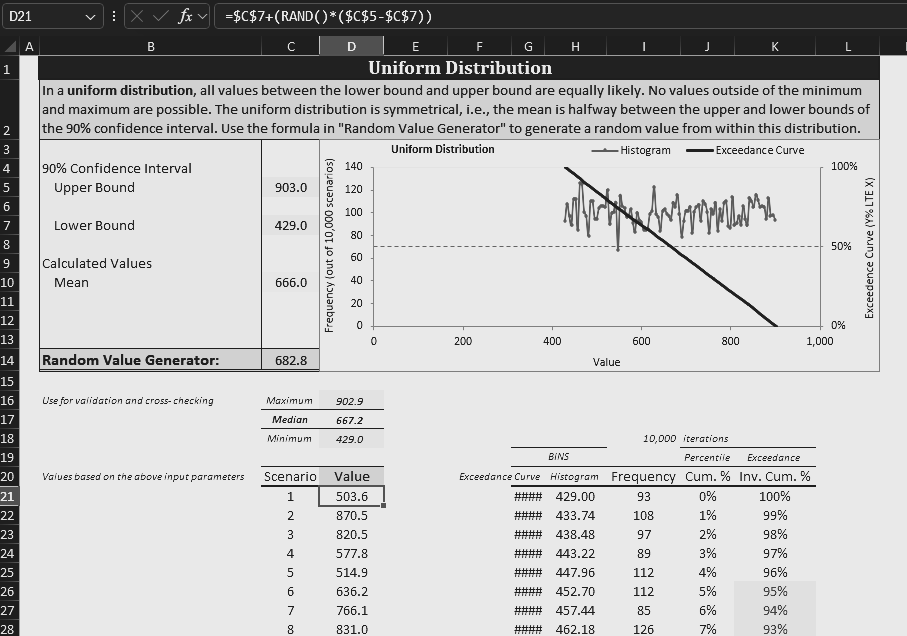
\includegraphics[width=\linewidth]{figures/Screenshot 2026-07-28 145652.png}}}
  \caption{Example run of a\index{simulation!Monte Carlo} Monte Carlo simulation using state-level data to set bounds.  Here we chose\index{Personal Data Breach} Personal Data Breach victim counts from 2016 and 2022 as upper and lower bounds. 10,000 rows projected randomized values between these bounds and determined mean and counts by\index{confidence interval} confidence interval.
  \protect\endnote{Monte Carlo Modeling Toolkit authored by Derek E. Brink, CISSP, \url{www.linkedin.com/in/derekbrink}. March 2023.}
  }
  \label{fig:screenshot-montecarlo1}
\end{figure}
\subsection{Background and Content}
We had a modest amount of education in\index{statistics} statistics as we began the project.  Our skills were derived primarily from three college courses.  At\index{Chattanooga}\index{Community College!Chattanooga State} Chattanooga State Community College in 2011, we had courses in "Elementary Statistics." \endnote{Triola, Mario F. Elementary Statistics Technology Update + Mystatlab Student Access Code Card. Pearson College Division, 2012.} This was an algebra-based course that focused on the fundamentals of applying data to normal distributions.  Also there in 2012, we had a course in "Statistics for Engineers." \endnote{Levine, David M, et al. Applied Statistics for Engineers and Scientists. Pearson, 2001.} This was an algebra-based course that discussed various quality control techniques and statistical modeling.  In 2023 at\index{University!Harvard!Extension School} Harvard University Extension School, we had a graduate course in "Risk in Information Security" with Derek Brink.  \endnote{Hubbard, Douglas W, and Richard Seiersen. How to Measure Anything in Cybersecurity Risk. Wiley, 2016.}  Professor Brink authored the Excel spreadsheet which we have used for\index{simulation!Monte Carlo} Monte Carlo simulations.

\begin{figure}[H]
  \centering
  \rotatebox{0}{\scalebox{1}{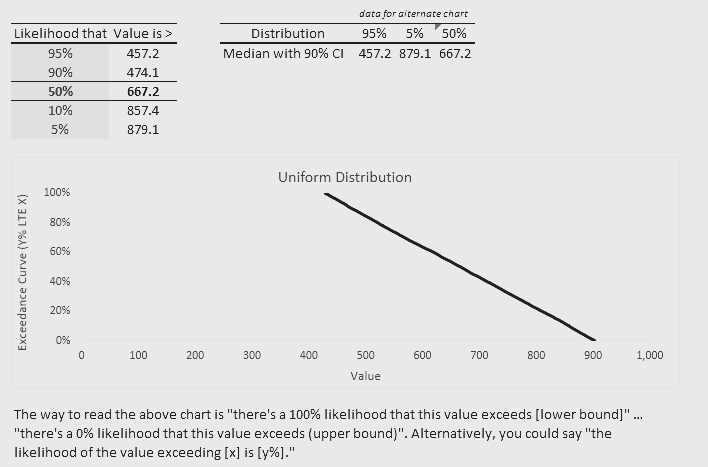
\includegraphics[width=\linewidth]{figures/Screenshot 2026-07-28 145609.png}}}
  \caption{Example results of applying\index{simulation!Monte Carlo} Monte Carlo simulation to forecasting.  Here we see the assertion that there is a 90\% likelihood that the number of victims will be between 457 and 879; the mean of the simulation was 667.\protect\endnote{Monte Carlo Modeling Toolkit authored by Derek E. Brink, CISSP, \url{www.linkedin.com/in/derekbrink}. March 2023.}}
  \label{fig:screenshot-montecarlo1}
\end{figure}

The spreadsheet conducts 10,000 simulations of data points between user-supplied bounds.  Sheets in the Excel workbook are capable of conducting a variety of these simulations.  They are differentiated by modeling style (uniform, triangular, normal, binary, or discrete) and points of interest (count, cost, or percentage).

Each of the simulating rows follows these general steps:
\begin{itemize}
\item{Reference the lower bound.}
\item{Ascertain the range between lower and upper bounds.}
\item{Generate a random number.}
\item{Multiply the random number against the range value.}
\item{Install the generated random value in a cell.}
\end{itemize}
The row values are then counted, sorted, and ranked into\index{confidence interval} confidence intervals.  The values and critical points are plotted on various graphs.  The end result is that it is easy for an opertor of the spreadsheet to generate a\index{simulation!Monte Carlo} Monte Carlo simulation of a distribution between bounds.  Since there are enough iterations (10,000), the simulation can have statistical value.  Since the inputs on the spreadsheet can be readily modified and since the cells are calculated upon page saving or loading, new simulations can be run with ease.  We recognized Professor Brink's spreadsheet was a useful tool that we could apply to forecasts of interest to us here.
\subsection{Problem Statement}
We need a cheap source of risk information to inform procedural decisions in the lab.  We can't afford to pay a vendor for intelligence feeds.  Free attack-specific feeds that work well for defense technologies like Snort or Suricata are not in a form that would inform policy-level risk decisions.  We want to gather this information efficiently and without generating any civil or criminal liability or threats; we're not going to conduct firsthand research in \index{cybercrime} cybercrime forums to determine what shape a localized risk might take.  We want to be able to  use publicly available \index{cybercrime} cybercrime data in order to persue commercial-grade decisions on a localized scale in a manner that is informed and practical.

These conditions suggest that we should use the following resources:
\begin{itemize}
  \item \gls{us} \gls{ic3} data
  \item \gls{cert} data from other nations
  \item\index{open data} Open Data from local government agencies
  \item MITRE ATT\&CK for guiding data selection
  \item Other scientifically valid\index{open data} Open Data sources.
\end{itemize}

We found during our research that there would sometimes be promising documents published by security vendors and software companies.  Unfortunately, many of those were not accompanied by scientifically valid\index{open data} open data sources.  So it is with caution that we could sometimes accept the assertions; however, we sometimes found that the reports were useless beyond identifying an anecdotal cause, condition, or effect.  Without data to quantify those identified conditions, we were sometimes left with a good idea that could not be proven in a manner that supported a\index{risk assessment!quantitative} quantitative risk assessment.  In those times, those leads had to sometimes be abandoned or be allowed to fall short of their potential impact.  Unscientific assertions from vendors seemed to be a trend in our research environment; unscientific assertions from vendors is such a part of the problem's environment that it is a problem almost unto itself.

\subsection{Project Objectives}
We want to be able to conduct a quantative risk assessment for our small project lab that would be scientific and illustrative enough to allow others to accept it as guidance.  

We want others to be able to conduct their own\index{risk assessment} risk assessments 
and be able to use these notes as a pattern for their own benefit.

We want to be able to use scaled-to-size \gls{ic3} data in a Monte Carlo simulation as a baseline for understanding the potential rates and severity of cybercrime encounters.

We want to proceed with an educated, professionally supported philosophical framework of ideas.  We didn't want to decay into philosophical edge cases like harshly questioning cause and effect, blindly ignoring unquantified threats, or emotionally fueling conspiratorial fears.  We need to keep our feet on the ground and our systems defended; but, if the\index{risk assessment} risk assessment shows that threats are rare or severe, then we need to understand that through quantitative analysis.

\subsubsection{Limits on Hypothesis Testing}
By themselves, the Monte Carlo simulations will allow us to make some narrow assertions, but for the statistics to have greater local benefit follow-on data gathering and analysis would be needed.  In this project we are scaling down national and state level data to a more localized scope.  However, that doesn't provide us with testable hypothesis.  These statistics could be used as a baseline for understanding the context of other treatments, measurements, or forecasts; but, by themselves, there will be little we can prove or disprove with our simulations.  We will be able to make simple assertions about the likelihood and severity of impact certain cybercrime types may have on our sample, but we will not be able to forecast the effectiveness of any local treatments, mitigations, or defensive techniques.

\subsection{Scope of Work}
We chose to limit our risk analysis to the algebraic scaling of \gls{ic3} data on Excel spreadsheets to limit the calculations by hand.  The data has four main trends (victim count, victim impact, suspect count, suspect impact), but to keep the analysis productive we would proceed all the way through with victim count.  This would support an assessment of likelihood.  Then we would go through the mathematics again to determine severity by scaling the values of victim impact.  With those two categories available, we would have the minimum amount of data needed to conduct a quantitative assessment of likelihood and severity.  This would meet the minimum expectations of most\index{risk assessment} risk assessments' data analysis needs.

We would need to scope the data to understand it in a verifiable context.  Since our goal is to analyze a project-sized scaling, we would need to couch that target between verifiable guideposts.  So, we chose to scale state-level data to our city's \index{population} population.  Alongside this, we could scale state-level data to a small organization's size (e.g. 150 people as stakeholders).  Since that scaled data would be calculated, we would want to present it in context with states and territories that represented high and low levels of \index{cybercrime} cybercrime (California and \index{American Samoa} American Samoa).  This way we would set a scope that would allow a reader to see the effect of scaling from known states down to the small business organization level.  
\subsection{Variables}
Not all of the collected \gls{ic3} data categories were stable over time.  As the reports were produced year to year, new threats emerged and the \index{cybercrime} cybercrime field changed.  This meant that some categories that were present at the older end of our analysis (2016) were not present at the end of our sampling (2022) or later.  Because of this, we had to ignore some categories or combine others.  Variability in criminal activity affected reporting.  

This had indirect effects on our analysis.  Check Fraud and Credit Card Fraud, as activity titles, changed over the years.  Threats to people, in the form of both Terrorism and Stalking, changed over the years.  This meant that we chose to ignore some categories that would seem to have value to commercial businesses while combining counts into one category in others.  Our picking and choosing among the categories genuinely shapes the risk picture we're considering as we do the\index{risk assessment} risk assessment.  Our projects and labs can't live in a fictional world where entire threat categories don't exist; but, we had to keep the data calculatable in order to proceed. 

\subsection{Assumptions, Risks, and Limitations}
We set out to better understand the rates of computer-related crimes in our area using public data sources.  We drew from FBI \gls{ic3} annual reports and\index{Chattanooga} Chattanooga Police\index{open data} open data records.  The \gls{ic3} reports provided categorical breakdowns of different types of internet-related crimes.  In the past, we were able to find per-state breakdowns of those crimes.  The FBI would provide four views of computer crime:  overall count, overall financial impact, victim count, and per-victim financial impact.  This was available both nationally and per state.  When following up in 2026, we noticed we were only able to immediately discover the national-level summaries of crime.

Anecdotally, we know that we have witnessed several of these crimes at rates higher than shown in these tables (Tables \ref{tab:chattanoogacrime2}, \ref{tab:chattanoogacrime3}, \ref{tab:chattanoogacrime4}).  We suspect that we're seeing numbers this low because few victims are taking the steps necessary to report computer crimes to federal authorities.  For example, when companies or individuals encounter ransomware, their reactions may involve repairing the afffected endpoint but not informing law enforcement.  Nonetheless, those authorities have been the public's observable source of crime reporting.  While we continue to use this data, we may need to accept that true counts of \index{cybercrime} cybercrime in the city must be scaled by an unknown factor.

The\index{Chattanooga}\index{Chattanooga!Police Department} Chattanooga Police Department, like other departments of the City of\index{Chattanooga} Chattanooga, participate in an\index{open data} open data project.  Anonymonized crime reports are provided to the public in a manner that lets us track by approximate region of the city and by category of crime.  We chose to do this because we recognized some crimes would be reported to local police that were not reported to federal authorities.  Some crimes, such as physical break-ins, were more likely to be handled by local police.  Since the systems involved are in-scope for physical damage, we felt the\index{Chattanooga}\index{Chattanooga!Police Department} Chattanooga Police Department's\index{open data} open data would be the best public source for supporting criminal threat forecasts for events like burglary from a vehicle.  Some of the crime categories, such as extortion or threats against a person, could be reported to either federal \gls{ic3} or local police; the nature of the threats might be different; but, there may be more direct physical threats reported to local police; there is no formal mimetic analysis that would shuttle a threatening complaint to one law enforcement agency or another.  Meanwhile, some locally policed crimes may focus upon:  employees, facility safeguards, loss of computer equipment in public, loss of computer equipment by theft from facilities or vehicles, and so on.  

As we examine the data from the public data sources and we feel that the reported rates are less than our experience would justify, we have to recognize that there may be shortcomings in the reported data.  Perhaps we would do well to scale the rates up to meet our experience.  However, those arbitrary inflations would damage the validity of our academic risk calculations.  So, for the time being, we leave the inflation or deflation of the end results for the reader as a localized adjustment.  Since our main goal is to show a method for determining the risks through the reported data, it could be argued that the exact numbers are less relevant than the demonstrated methods.
\subsubsection{Limitations Imposed by Federal Law Enforcement in Tennessee}
During our research, one shocking fact came to light.  At the Cybersecurity Summit conference in Nashville, TN in 2023, Derek Rousseau, a Special Agent from the FBI Nashville Cyber Squad, presented and answered a Q\&A.  To our surprise, the special agent answered a direct question, How much money needs to be at stake for the \gls{fbi} to get involved in a \index{cybercrime} cybercrime?  His answer was that the US Attorney in Nashville wanted to see at least \$100,000 in damage for domestic crimes or \$400,000 in damage for international crimes.  For damage amounts below that, it was not effective to devote an \gls{fbi} special agent to investigate the crime.  As a result, the special agent encouraged the reporting of smaller crimes so that cases could be aggregated against a suspect to levels that merited federal investigation and prosecution.  Later, as we compare \gls{ic3} crime data, we'll see that many of the annual totals are below these limits.  This suggests that the \gls{us} is prosecuting only a fraction of those reported crimes that affect the \index{population} population.
\subsubsection{Limitations Derived from Reporting}
Another limitation on our projections arises from the voluntary nature of the reporting.  Since victims or defenders need to advise the \gls{ic3} of a security event, only those who follow through with the voluntary reporting actions will get counted.  Commercial defenders will see that in their experience only a small number of daily cybersecurity events will seem worthy to report to federal law enforcement; the scope of true attacks would seem through those anecdotes to be much greater than the reported numbers.  Since all of the reports are likely to be initiated by those who speak up, we cannot escape the experimental design problems associated with a\index{sample!convenience} convenience sample when using \gls{ic3} data for our\index{statistics} statistics.

As we've seen and will see, the grouping of those reports does not match our experimental needs.  States and nations are simply too large to be of practical benefit to defenders.  Most small businesses and organizations will need the value of public information; commercial vendors can provide similar data for a fee; we need the free data, but we need to tailor it down to the size of a defending organization to apply it realistically to\index{risk assessment} risk assessments for cybersecurity defense.
\subsection{Significance of the Project}
We hope to take the mystery out of public\index{statistics} statistics for cybersecurity use.  We want to provide the types of workshop examples we've seen locally in\index{open data} open data workshops \endnote{"City of Chattanooga Hub." Chattanooga.Gov, 2025, \url{https://data.chattanooga.gov/}. Accessed 4 Aug. 2026.} but in technical note form.  Ideally, readers should be able to follow these notes and then craft their own projects for forecasting cybersecurity risk using publicly available data sources.
\section{Literature Review}
\subsection{Overview of Existing Solutions or Approaches}
\subsection{Comparisons of Technologies or Frameworks}
\subsection{Gaps in the Literature}
We haven't found many examples outside of college classrooms that allow readers to follow the extrapolation process and formulate their own forecasts for cybersecurity risks.  While there are excellent books on the topics of\index{statistics} statistics and cybersecurity, we havent' found works that took public data like this and used it for other purposes.  

In our hometown of\index{Chattanooga} Chattanooga, there have been public non-profit efforts to use\index{open data} open data in workshops that are free and open to the public.  Most of the data sets used for those activities are part of local government's participation in an\index{open data} open data initiative. \endnote{"City of Chattanooga Hub." Chattanooga.Gov, 2025, \url{https://data.chattanooga.gov/}} By working through Jupyter notebooks and group discussions, participants might learn more about public bicycle rental use, for example.  Our interests, meanwhile, lay firmly within the cybersecurity realm.  
\section{Methodology}
\begin{figure}[H]
  \centering
  \rotatebox{0}{\scalebox{1}{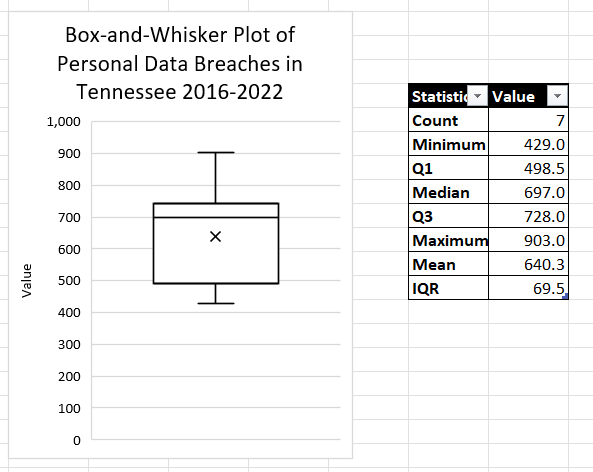
\includegraphics[width=\linewidth]{figures/boxwhisker-tnpersdatabreach2016.png}}}
  \caption{Seven year summary of\index{Personal Data Breach} Personal Data Breaches in Tennessee reported to \gls{ic3}. }
  \label{fig:screenshot-boxwhisker-tnpersdatabreach2016}
\end{figure}
We took \index{cybercrime} cybercrime data from a seven year span of \gls{ic3} publications.  The annual reports for the nation and for each state showed a count of victims per category of \index{cybercrime} cybercrime.  The \gls{us} \gls{fbi} defined each category for their report.  We put that data into a matrix, organized by year and category of crime.  

Each state we chose got its own matrix. We noticed that three states typically had high counts of crime; they were: \index{California} California,\index{Texas} Texas, and\index{Florida} Florida.  We noticed that US territories, like \index{American Samoa} American Samoa, US Virgin Islands, and\index{Puerto Rico} Puerto Rico, were reported also as if they were a state.  These smaller areas with lower \index{population} populations also showed lowed low counts of \index{cybercrime} cybercrime.  We chose these high crime areas (e.g.\index{California} California) and low crime areas (e.g. \index{American Samoa} American Samoa) as our guides for choosing maximum and minimum limits.  Our desired target areas were chosen by the target's home state; our intial runs included \index{Chattanooga} Chattanooga, Tennessee.

\subsection{Using State Data to Forecast a Company's Data}

Our main data sets are provided in the public interest; they're based on large units of people like states and nations.  As system operators, we have a much smaller interest; we're interested in company sized elements.  Instead of being concerned with the \index{cybercrime} cybercrime fate of over 300 million Americans or 9 million Tennesseans, we are probably more interested in what might happen to 100 stakeholders.  

To smooth out the counts of \index{cybercrime} cybercrime into rates, we adjusted these state victim counts per capita.  We chose the\index{US Census} US Census reports for those years to be the \index{population} population values of the states.  This would provide us with a per capita rate of \index{cybercrime} cybercrime based on the chosen state which represented the chosen limit or target in the distribution.

Formally, we note this process below as shown in Figure \ref{fig:statcalc-percap}.  $R$ represents our result.  $N_t$ represents our constant for target \index{sample} sample \index{population} population and is used for multiplying the rate to scale it to match the \index{population} population of the target. $t$ represents our starting year for the \index{sample} sample from \gls{ic3} and coordinates the rows until it progresses to the final year chosen which is denoted by $n$. $i$ represents our chosen category index of \index{cybercrime} cybercrime. $j$ represents our year index and is built with $t$ until it progresses to the final year of the \index{sample} sample denoted by $n$. $P_j$ represents the \index{population} population of the target city at year $j$, drawn from matrix $P$.

\begin{figure}[H]
  \centering




\[
R_j = N_t \sum_{j=t}^{t+6} \frac{X_{j,i}}{P_j}, \quad \text{where } X_{j,i} = \begin{cases} M_{j,i} & \text{if victim count} \\ V_{j,i} & \text{if victim impact} \\ S_{j,i} & \text{if suspect count} \\ D_{j,i} & \text{if suspect impact} \end{cases}
\]

  \caption{Notation for the statistical calculation of the security event matrix adjusted for per-capita rates of incidence.}
  \label{fig:statcalc-percap}
\end{figure}

Five matrices inform this calculation.  The first, $P$ as shown in Figure \ref{fig:statcalc-popmatrix}, records the target city \index{population} population for each year of the \index{sample} sample as a single column.

\begin{figure}[H]
  \centering

\[
P=
\text{Years }\left\{
\begin{matrix}
t\\ \vdots\\ j\\ \vdots\\ n
\end{matrix}
\right.
\left[
\begin{array}{c}
\multicolumn{1}{c}{%
  \overbrace{\hphantom{p_{t}}}^{\text{Population}}%
}\\
p_t \\
\vdots \\
p_j \\
\vdots \\
p_n
\end{array}
\right]
\]

  \caption{Structure of the \index{sample} sample \index{population} population matrix indexed by year.}
  \label{fig:statcalc-popmatrix}
\end{figure}

The second matrix, $M$ as shown in Figure \ref{fig:statevent-victimcount}, organises the raw \index{cybercrime} cybercrime counts from \gls{ic3} by category and year, where each entry $a_{j,i}$ is a count that will be adjusted to a per-capita rate.


\begin{figure}[H]
  \centering
\[
M=
\text{Years }\left\{
\begin{matrix}
t\\ \vdots\\ j\\ \vdots\\ n
\end{matrix}
\right.
\left[
\begin{array}{ccccccc}
\multicolumn{7}{c}{%
  \overbrace{%
    \hphantom{a_{t,1}\ \cdots\ a_{t,2}\ \cdots\ a_{t,i}\ \cdots\ a_{t,m}}%
  }^{\text{Victim Counts by Categories}}%
}\\
a_{t,1} & \cdots & a_{t,2} & \cdots & a_{t,i} & \cdots & a_{t,m} \\
\vdots  & \ddots & \vdots  & \ddots & \vdots  & \ddots & \vdots \\
a_{j,1} & \cdots & a_{j,2} & \cdots & a_{j,i} & \cdots & a_{j,m} \\
\vdots  & \ddots & \vdots  & \ddots & \vdots  & \ddots & \vdots \\
a_{n,1} & \cdots & a_{n,2} & \cdots & a_{n,i} & \cdots & a_{n,m}
\end{array}
\right]
\]

  \caption{Structure of the security event matrix for victim counts by \index{cybercrime} cybercrime categories indexed by year.}
  \label{fig:statevent-victimcount}
\end{figure}


The third matrix, $V$ as shown in Figure \ref{fig:statevent-victimimpact}, organises the victim impact in USD from \gls{ic3} by category and year, where each entry $a_{j,i}$ is a count that will be adjusted later to a per-capita rate.
\begin{figure}[H]
  \centering
\[
V=
\text{Years }\left\{
\begin{matrix}
t\\ \vdots\\ j\\ \vdots\\ n
\end{matrix}
\right.
\left[
\begin{array}{ccccccc}
\multicolumn{7}{c}{%
  \overbrace{%
    \hphantom{a_{t,1}\ \cdots\ a_{t,2}\ \cdots\ a_{t,i}\ \cdots\ a_{t,m}}%
  }^{\text{Victim Impacts by Categories}}%
}\\
a_{t,1} & \cdots & a_{t,2} & \cdots & a_{t,i} & \cdots & a_{t,m} \\
\vdots  & \ddots & \vdots  & \ddots & \vdots  & \ddots & \vdots \\
a_{j,1} & \cdots & a_{j,2} & \cdots & a_{j,i} & \cdots & a_{j,m} \\
\vdots  & \ddots & \vdots  & \ddots & \vdots  & \ddots & \vdots \\
a_{n,1} & \cdots & a_{n,2} & \cdots & a_{n,i} & \cdots & a_{n,m}
\end{array}
\right]
\]


  \caption{Structure of the security event matrix for victim impacts, as in dollars of damage, by \index{cybercrime} cybercrime categories indexed by year.}
  \label{fig:statevent-victimimpact}
\end{figure}

The fourth matrix, $S$ as shown in Figure \ref{fig:statevent-suspectcount}, organises the count of suspects from \gls{ic3} by category and year.  Each entry $a_{j,i}$ helps us to understand how many suspects are operating within an area of concern.  This is a count that will be adjusted later to a per-capita rate.

\begin{figure}[H]
  \centering
\[
S=
\text{Years }\left\{
\begin{matrix}
t\\ \vdots\\ j\\ \vdots\\ n
\end{matrix}
\right.
\left[
\begin{array}{ccccccc}
\multicolumn{7}{c}{%
  \overbrace{%
    \hphantom{a_{t,1}\ \cdots\ a_{t,2}\ \cdots\ a_{t,i}\ \cdots\ a_{t,m}}%
  }^{\text{Suspect Counts by Categories}}%
}\\
a_{t,1} & \cdots & a_{t,2} & \cdots & a_{t,i} & \cdots & a_{t,m} \\
\vdots  & \ddots & \vdots  & \ddots & \vdots  & \ddots & \vdots \\
a_{j,1} & \cdots & a_{j,2} & \cdots & a_{j,i} & \cdots & a_{j,m} \\
\vdots  & \ddots & \vdots  & \ddots & \vdots  & \ddots & \vdots \\
a_{n,1} & \cdots & a_{n,2} & \cdots & a_{n,i} & \cdots & a_{n,m}
\end{array}
\right]
\]

  \caption{Structure of the security event matrix for suspect counts by \index{cybercrime} cybercrime categories indexed by year.  These counts consider the number of actors who engage victims in a given area.}
  \label{fig:statevent-suspectcount}
\end{figure}

The fifth matrix, $D$ as shown in Figure \ref{fig:statevent-suspectdamage}, organises the damages attributed by suspects in USD from \gls{ic3} by category and year, where each entry $a_{j,i}$ is a count that will be adjusted later to a per-capita rate.  This helps us to understand rates of effective impact, per suspect, in a given area.

\begin{figure}[H]
  \centering
\[
D=
\text{Years }\left\{
\begin{matrix}
t\\ \vdots\\ j\\ \vdots\\ n
\end{matrix}
\right.
\left[
\begin{array}{ccccccc}
\multicolumn{7}{c}{%
  \overbrace{%
    \hphantom{a_{t,1}\ \cdots\ a_{t,2}\ \cdots\ a_{t,i}\ \cdots\ a_{t,m}}%
  }^{\text{Suspect Damage by Categories}}%
}\\
a_{t,1} & \cdots & a_{t,2} & \cdots & a_{t,i} & \cdots & a_{t,m} \\
\vdots  & \ddots & \vdots  & \ddots & \vdots  & \ddots & \vdots \\
a_{j,1} & \cdots & a_{j,2} & \cdots & a_{j,i} & \cdots & a_{j,m} \\
\vdots  & \ddots & \vdots  & \ddots & \vdots  & \ddots & \vdots \\
a_{n,1} & \cdots & a_{n,2} & \cdots & a_{n,i} & \cdots & a_{n,m}
\end{array}
\right]
\]

  \caption{Structure of the security event matrix for suspect damage, in dollars by perpetrators, by \index{cybercrime} cybercrime categories indexed by year.  This tally helps us understand how damaging each actor is to victims.}
  \label{fig:statevent-suspectdamage}
\end{figure}


We apply these matrices to the formula shown in Figure \ref{fig:statcalc-percap}. The entries $a_{j,i}$ are the raw counts taken from the \gls{ic3} state-level reports for the chosen source state.  Dividing each entry by $P_j$ converts it to a per-capita rate; multiplying by $N_t$ then scales that rate to match the \index{population} population of the target city.  The \index{population} population values in $P$ provide the year-by-year context for $N_t$ and confirm the representativeness of the scaling.  Summing the selected column $i$ of the per-capita-adjusted $M$ across all years yields the final result $R$.


\begin{table}[H]
  \centering
  \caption{Changes to \index{population} population in Key Areas}
  \label{tab:chattanoogacrime1}
  \begin{tabular}{@{}>{\centering\arraybackslash}
  p{0.15\linewidth} >{\centering\arraybackslash}
  p{0.07\linewidth}>{\centering\arraybackslash}
  p{0.07\linewidth}>{\centering\arraybackslash}
  p{0.07\linewidth}>{\centering\arraybackslash}
  p{0.07\linewidth}>{\centering\arraybackslash}
  p{0.07\linewidth}>{\centering\arraybackslash}
  p{0.07\linewidth}>{\centering\arraybackslash}
  p{0.07\linewidth}>{\centering\arraybackslash}
  p{0.07\linewidth}}
    \toprule
    \textbf{Year} & 
    \rotatebox{90}{\begin{tabular}{@{}ll@{}}\index{American Samoa} American Samoa\\Population\end{tabular}} &
    \rotatebox{90}{\begin{tabular}{@{}ll@{}}References\end{tabular}} &
    \rotatebox{90}{\begin{tabular}{@{}ll@{}}City of \index{Chattanooga} Chattanooga\\Population\end{tabular}} &
    \rotatebox{90}{\begin{tabular}{@{}ll@{}}References\end{tabular}} &
    \rotatebox{90}{\begin{tabular}{@{}ll@{}}State of Tennessee\\Population\end{tabular}} &
    \rotatebox{90}{\begin{tabular}{@{}ll@{}}References\end{tabular}} &
    \rotatebox{90}{\begin{tabular}{@{}ll@{}}State of\index{California} California\\Population\end{tabular}} &
    \rotatebox{90}{\begin{tabular}{@{}ll@{}}References\end{tabular}} 

    \\
    \midrule
2016&&&177,746&\endnote{\url{https://www.census.gov/quickfacts/chattanoogacitytennessee}}&6,646,010&\endnote{\url{https://www.census.gov/quickfacts/fact/table/TN/PST045222}}\\
2017&&&179,530&\endnote{\url{https://www.census.gov/quickfacts/chattanoogacitytennessee}}&6,708,799&\endnote{\url{https://www.census.gov/quickfacts/fact/table/TN/PST045222}}\\
2018&&&181,918&\endnote{\url{https://www.census.gov/quickfacts/chattanoogacitytennessee}}&6,771,631&\endnote{\url{https://www.census.gov/quickfacts/fact/table/TN/PST045222}}\\
2019&&&182,799&\endnote{\url{https://www.census.gov/quickfacts/chattanoogacitytennessee}}&6,829,174&\endnote{\url{https://www.census.gov/quickfacts/fact/table/TN/PST045222}}\\
2020&&&181,560&\endnote{\url{https://www.census.gov/quickfacts/chattanoogacitytennessee}}&6,925,619&\endnote{\url{https://www2.census.gov/programs-surveys/popest/datasets/2020-2022/state/totals/NST-EST2022-POPCHG2020_2022.csv}}\\
2021&&&181,163&\endnote{\url{https://www.census.gov/quickfacts/chattanoogacitytennessee}}&6,968,351&\endnote{\url{https://www2.census.gov/programs-surveys/popest/datasets/2020-2022/state/totals/NST-EST2022-POPCHG2020_2022.csv}}\\
2022&&&184,086&\endnote{\url{https://www.census.gov/quickfacts/chattanoogacitytennessee}}&7,051,339&\endnote{\url{https://www2.census.gov/programs-surveys/popest/datasets/2020-2022/state/totals/NST-EST2022-POPCHG2020_2022.csv}}\\

    \bottomrule \end{tabular} 
\raggedright{City \index{population} population based on the\index{US Census} US Census reported \index{population} population for the City of\index{Chattanooga} Chattanooga itself.  Surrounding satellite cities and unincorporated areas within the Hamilton County, Tennessee, were not included. \index{population} population for the State of Tennessee provided perspective on calculated rates in later tables. \index{population} population for \index{American Samoa} American Samoa and the State of\index{California} California were included for perspective on maximum and minimum counts in later tables.}
\end{table}


\subsubsection{Corporate and Personal Data Breaches}

\begin{table}[H]
  \centering
  \caption{Projected In-City Victim Counts, City of\index{Chattanooga} Chattanooga, Threats to System Intrusion}
  \label{tab:chattanoogacrime2}
  \begin{tabular}{@{}>{\centering\arraybackslash}
  p{0.05\linewidth} >{\centering\arraybackslash}
  p{0.35\linewidth}>{\centering\arraybackslash}
  p{0.35\linewidth}>{\centering\arraybackslash}
  p{0.05\linewidth}}
    \toprule
    Year
    &Data Breach
    &Personal Data Breach
    &\\
    \midrule
        

2016&1&11&\endnote{original\url{https://www.ic3.gov/Media/PDF/AnnualReport/2016State/StateReport.aspx\#?s=47} current \url{https://www.ic3.gov/AnnualReport/Reports/2016_IC3Report.pdf}}\\
2017&1&13&\endnote{original:\url{https://www.ic3.gov/Media/PDF/AnnualReport/2017State/StateReport.aspx\#?s=47} current: \url{https://www.ic3.gov/AnnualReport/Reports/2017_IC3Report.pdf}}\\
2018&0&18&\endnote{original:\url{https://www.ic3.gov/Media/PDF/AnnualReport/2018State/StateReport.aspx\#?s=47} current: \url{https://www.ic3.gov/AnnualReport/Reports/2018_IC3Report.pdf}}\\
2019&0&13&\endnote{original:\url{https://www.ic3.gov/Media/PDF/AnnualReport/2019State/StateReport.aspx\#?s=47} current: \url{https://www.ic3.gov/AnnualReport/Reports/2019_IC3Report.pdf}}\\
2020&0&18&\endnote{original:\url{https://www.ic3.gov/Media/PDF/AnnualReport/2020State/StateReport.aspx\#?s=47} current: \url{https://www.ic3.gov/AnnualReport/Reports/2020_IC3Report.pdf}}\\
2021&0&19&\endnote{original:\url{https://www.ic3.gov/Media/PDF/AnnualReport/2021State/StateReport.aspx\#?s=47} current: \url{https://www.ic3.gov/AnnualReport/Reports/2021_IC3Report.pdf}}\\
2022&1&23&\endnote{original:\url{https://www.ic3.gov/Media/PDF/AnnualReport/2022State/StateReport.aspx\#?s=47} current: \url{https://www.ic3.gov/AnnualReport/Reports/2022_IC3Report.pdf}}\\

    \bottomrule \end{tabular} 
  \raggedright{Counts deduced from IC3 Victim Complaints for Tennessee adjusted for a per-capita rate and then multiplied by the city's \index{population} population for that year.}
\end{table}
\begin{figure}[H]
  \centering
  \rotatebox{0}{\scalebox{1}{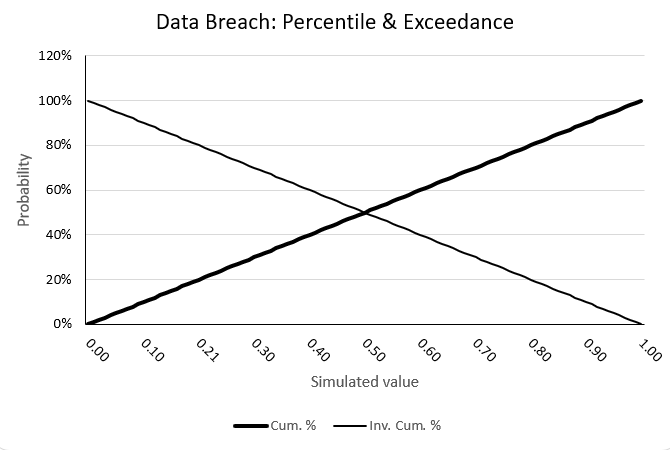
\includegraphics[width=\linewidth]{figures/Screenshot 2026-08-05 093747.png}}}
  \caption{A\index{simulation!Monte Carlo} Monte Carlo simulation suggests that there is a 50\% probability that 0.5 or more\index{data breach} data breaches will occur within the \index{sample} sample.  This unusual result is because the confidence bounds are between 0 and 1.  We interpret this as a 50\% probability that one data breach will occur. \protect\endnote{\index{sample} Sample size was set equivalent to the City of\index{Chattanooga} Chattanooga to determine the per capita rates for each year over data from \index{American Samoa} American Samoa and\index{California} California.  The medians of those rates were used to set 10\% and 90\%\index{confidence interval} confidence intervals with \index{American Samoa} American Samoa and\index{California} California representing low and high \index{cybercrime} cybercrime counts respectively.}
  \protect\endnote{Monte Carlo Modeling Toolkit authored by Derek E. Brink, CISSP, \url{www.linkedin.com/in/derekbrink}. March 2023.}
  }
  \label{fig:screenshot-montecarlopersdatabreachexceedence}
\end{figure}

\begin{figure}[H]
  \centering
  \rotatebox{0}{\scalebox{1}{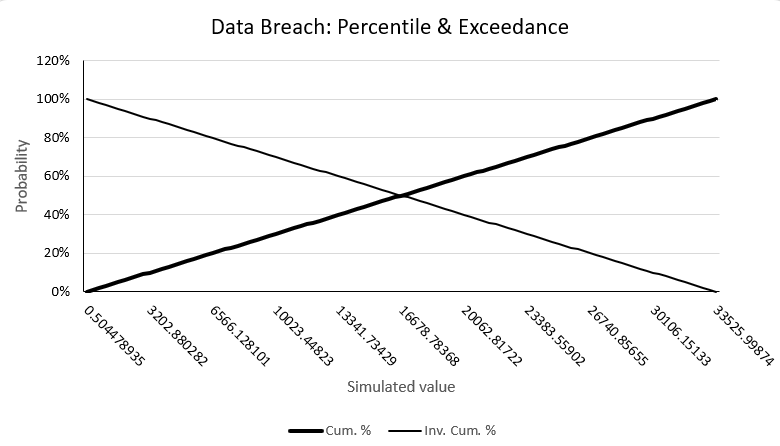
\includegraphics[width=\linewidth]{figures/Screenshot 2026-08-05 092857.png}}}
  \caption{A\index{simulation!Monte Carlo} Monte Carlo simulation suggests that there is a 90\% probability that\index{data breach} data breaches will cost \$3,202 or more in a year.  There is a 50\% likelihood that they will cost \$16,678 or more in a year.  There is a 10\% chance that they will cost \$30,106 or more in a year. \protect\endnote{\index{sample} sample size was set equivalent to the City of\index{Chattanooga} Chattanooga to determine the per capita rates for each year over data from \index{American Samoa} American Samoa and\index{California} California.  The medians of those rates were used to set 10\% and 90\%\index{confidence interval} confidence intervals with \index{American Samoa} American Samoa and\index{California} California representing low and high \index{cybercrime} cybercrime impact values respectively.}
  \protect\endnote{Monte Carlo Modeling Toolkit authored by Derek E. Brink, CISSP, \url{www.linkedin.com/in/derekbrink}. March 2023.}
  }
  \label{fig:screenshot-montecarlopersdatabreachimpact}
\end{figure}
\begin{figure}[H]
  \centering
  \rotatebox{0}{\scalebox{1}{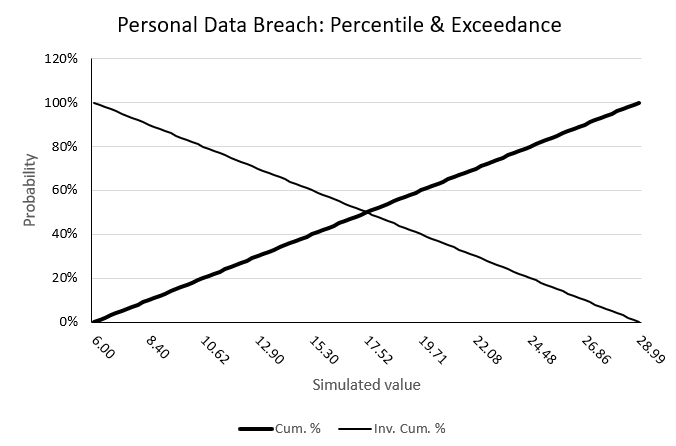
\includegraphics[width=\linewidth]{figures/Screenshot 2026-08-03 143039.png}}}
  \caption{A\index{simulation!Monte Carlo} Monte Carlo simulation suggests that there is a 90\% probability that 8 or more\index{Personal Data Breach} Personal Data Breaches will occur within the \index{sample} sample.  There is a 50\% likelihood that 17 or more will occur.  There is a 10\% chance that 26 or more will occur. \protect\endnote{\index{sample} Sample size was set equivalent to the City of\index{Chattanooga} Chattanooga to determine the per capita rates for each year over data from \index{American Samoa} American Samoa and\index{California} California.  The medians of those rates were used to set 10\% and 90\%\index{confidence interval} confidence intervals with \index{American Samoa} American Samoa and\index{California} California representing low and high \index{cybercrime} cybercrime counts respectively.}
  \protect\endnote{Monte Carlo Modeling Toolkit authored by Derek E. Brink, CISSP, \url{www.linkedin.com/in/derekbrink}. March 2023.}
  }
  \label{fig:screenshot-montecarlopersdatabreachexceedence}
\end{figure}

\begin{figure}[H]
  \centering
  \rotatebox{0}{\scalebox{1}{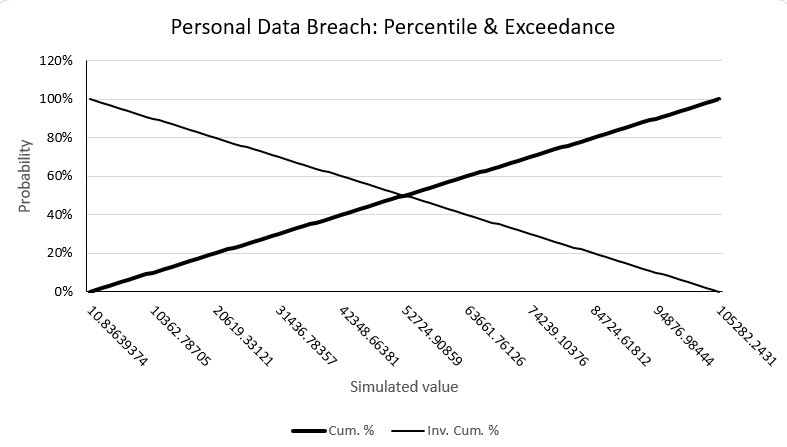
\includegraphics[width=\linewidth]{figures/Screenshot 2026-08-03 212425.png}}}
  \caption{A\index{simulation!Monte Carlo} Monte Carlo simulation suggests that there is a 90\% probability that\index{Personal Data Breach} Personal Data Breaches will cost \$10,362 or more in a year.  There is a 50\% likelihood that they will cost \$52,724 or more in a year.  There is a 10\% chance that they will cost \$94,876 or more in a year. \protect\endnote{\index{sample} sample size was set equivalent to the City of\index{Chattanooga} Chattanooga to determine the per capita rates for each year over data from \index{American Samoa} American Samoa and \index{California} California.  The medians of those rates were used to set 10\% and 90\% \index{confidence interval} confidence intervals with \index{American Samoa} American Samoa and\index{California} California representing low and high \index{cybercrime} cybercrime impact values respectively.}
  \protect\endnote{Monte Carlo Modeling Toolkit authored by Derek E. Brink, CISSP, \url{www.linkedin.com/in/derekbrink}. March 2023.}
  }
  \label{fig:screenshot-montecarlopersdatabreachimpact}
\end{figure}
\subsubsection{Threats to System Intrusion}
\begin{table}[H]
  \centering
  \caption{Projected In-City Victim Counts, City of\index{Chattanooga} Chattanooga, Threats to System Intrusion}
  \label{tab:chattanoogacrime3}
  \begin{tabular}{@{}>{\centering\arraybackslash}p{0.05\linewidth} >{\centering\arraybackslash}
  p{0.25\linewidth}>{\centering\arraybackslash}
  p{0.25\linewidth}>{\centering\arraybackslash}
  p{0.25\linewidth}>{\centering\arraybackslash}
  p{0.05\linewidth}}
    \toprule
    Year
    &Malware
    &Phishing
    &Ransomware
    &\\
    \midrule
        

2016&1&7&1&\endnote{original\url{https://www.ic3.gov/Media/PDF/AnnualReport/2016State/StateReport.aspx\#?s=47} current \url{https://www.ic3.gov/AnnualReport/Reports/2016_IC3Report.pdf}}\\
2017&1&9&0&\endnote{original:\url{https://www.ic3.gov/Media/PDF/AnnualReport/2017State/StateReport.aspx\#?s=47} current: \url{https://www.ic3.gov/AnnualReport/Reports/2017_IC3Report.pdf}}\\
2018&0&8&0&\endnote{original:\url{https://www.ic3.gov/Media/PDF/AnnualReport/2018State/StateReport.aspx\#?s=47} current: \url{https://www.ic3.gov/AnnualReport/Reports/2018_IC3Report.pdf}}\\
2019&1&8&0&\endnote{original:\url{https://www.ic3.gov/Media/PDF/AnnualReport/2019State/StateReport.aspx\#?s=47} current: \url{https://www.ic3.gov/AnnualReport/Reports/2019_IC3Report.pdf}}\\
2020&0&9&0&\endnote{original:\url{https://www.ic3.gov/Media/PDF/AnnualReport/2020State/StateReport.aspx\#?s=47} current: \url{https://www.ic3.gov/AnnualReport/Reports/2020_IC3Report.pdf}}\\
2021&0&11&1&\endnote{original:\url{https://www.ic3.gov/Media/PDF/AnnualReport/2021State/StateReport.aspx\#?s=47} current: \url{https://www.ic3.gov/AnnualReport/Reports/2021_IC3Report.pdf}}\\
2022&0&7&0&\endnote{original:\url{https://www.ic3.gov/Media/PDF/AnnualReport/2022State/StateReport.aspx\#?s=47} current: \url{https://www.ic3.gov/AnnualReport/Reports/2022_IC3Report.pdf}}\\

    \bottomrule \end{tabular} 
  \raggedright{Counts deduced from IC3 Victim Complaints for Tennessee adjusted for a per-capita rate and then multiplied by the city's \index{population} population for that year.}
\end{table}

\begin{figure}[H]
  \centering
  \rotatebox{0}{\scalebox{1}{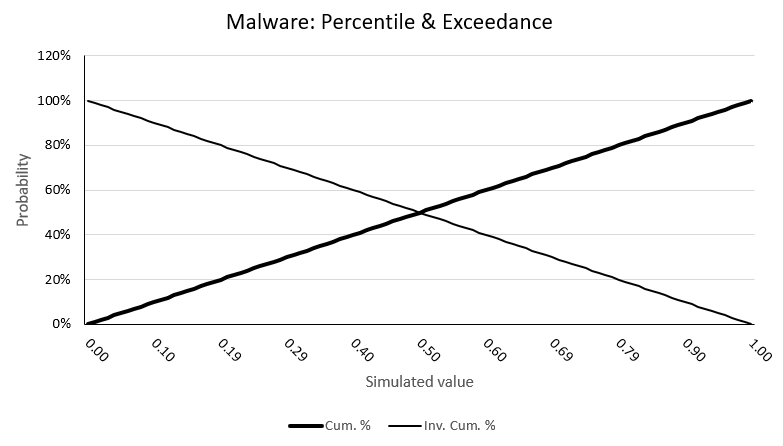
\includegraphics[width=\linewidth]{figures/Screenshot 2026-08-06 090519.png}}}
  \caption{The Monte Carlo simulation determined that there would be a 50\% chance of malware.  \protect\endnote{\index{sample} sample size was set equivalent to the City of\index{Chattanooga} Chattanooga to determine the per capita rates for each year over data from \index{American Samoa} American Samoa and \index{California} California.  The medians of those rates were used to set 10\% and 90\% \index{confidence interval} confidence intervals with \index{American Samoa} American Samoa and\index{California} California representing low and high \index{cybercrime} cybercrime impact values respectively.}
  \protect\endnote{Monte Carlo Modeling Toolkit authored by Derek E. Brink, CISSP, \url{www.linkedin.com/in/derekbrink}. March 2023.}
  }
  \label{fig:screenshot-montecarlopersdatabreachimpact}
\end{figure}

\begin{figure}[H]
  \centering
  \rotatebox{0}{\scalebox{1}{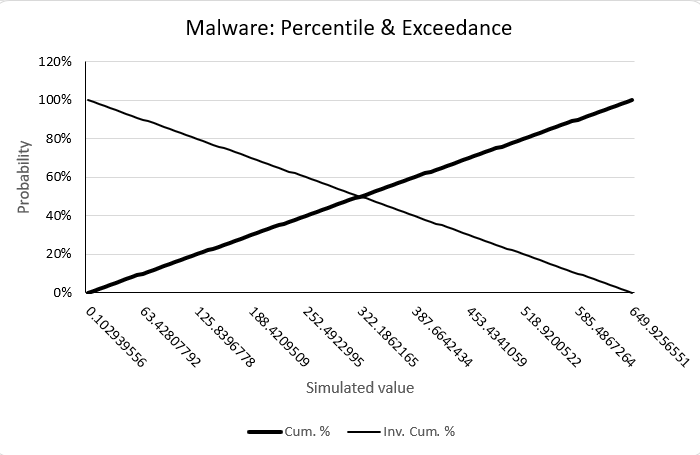
\includegraphics[width=\linewidth]{figures/Screenshot 2026-08-06 090805.png}}}
  \caption{A\index{simulation!Monte Carlo} Monte Carlo simulation suggests that there is a 90\% probability that\index{malware} malware will cost \$63 or more in a year.  There is a 50\% likelihood that they will cost \$322 or more in a year.  There is a 10\% chance that they will cost \$585 or more in a year. \protect\endnote{\index{sample} sample size was set equivalent to the City of\index{Chattanooga} Chattanooga to determine the per capita rates for each year over data from \index{American Samoa} American Samoa and \index{California} California.  The medians of those rates were used to set 10\% and 90\% \index{confidence interval} confidence intervals with \index{American Samoa} American Samoa and\index{California} California representing low and high \index{cybercrime} cybercrime impact values respectively.}
  \protect\endnote{Monte Carlo Modeling Toolkit authored by Derek E. Brink, CISSP, \url{www.linkedin.com/in/derekbrink}. March 2023.}
  }
  \label{fig:screenshot-montecarlopersdatabreachimpact}
\end{figure}

\begin{figure}[H]
  \centering
  \rotatebox{0}{\scalebox{1}{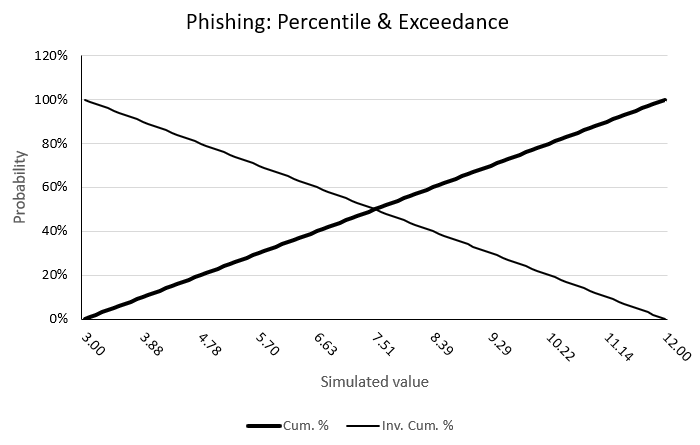
\includegraphics[width=\linewidth]{figures/Screenshot 2026-08-06 091252.png}}}
  \caption{The Monte Carlo simulation determined that there would be a 90\% chance of 3 or more index{phishing} phishing events.  There was a 50\% chance of 7 or more index{phishing} phishing events.  There was a 10\% chance of 11 or more events.  \protect\endnote{\index{sample} sample size was set equivalent to the City of\index{Chattanooga} Chattanooga to determine the per capita rates for each year over data from \index{American Samoa} American Samoa and \index{California} California.  The medians of those rates were used to set 10\% and 90\% \index{confidence interval} confidence intervals with \index{American Samoa} American Samoa and\index{California} California representing low and high \index{cybercrime} cybercrime impact values respectively.}
  \protect\endnote{Monte Carlo Modeling Toolkit authored by Derek E. Brink, CISSP, \url{www.linkedin.com/in/derekbrink}. March 2023.}
  }
  \label{fig:screenshot-montecarlopersdatabreachimpact}
\end{figure}

\begin{figure}[H]
  \centering
  \rotatebox{0}{\scalebox{1}{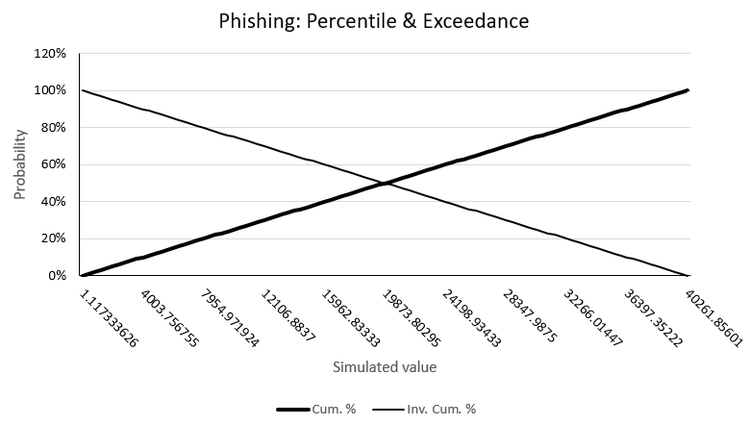
\includegraphics[width=\linewidth]{figures/Screenshot 2026-08-06 091913.png}}}
  \caption{A\index{simulation!Monte Carlo} Monte Carlo simulation suggests that there is a 90\% probability that\index{phishing} phishing events will cost \$4003 or more in a year.  There is a 50\% likelihood that they will cost \$19,873 or more in a year.  There is a 10\% chance that they will cost \$36,397 or more in a year. \protect\endnote{\index{sample} sample size was set equivalent to the City of\index{Chattanooga} Chattanooga to determine the per capita rates for each year over data from \index{American Samoa} American Samoa and \index{California} California.  The medians of those rates were used to set 10\% and 90\% \index{confidence interval} confidence intervals with \index{American Samoa} American Samoa and\index{California} California representing low and high \index{cybercrime} cybercrime impact values respectively.}
  \protect\endnote{Monte Carlo Modeling Toolkit authored by Derek E. Brink, CISSP, \url{www.linkedin.com/in/derekbrink}. March 2023.}
  }
  \label{fig:screenshot-montecarlopersdatabreachimpact}
\end{figure}
\subsubsection{Threats to Personnel}
\begin{table}[H]
  \centering
  \caption{Projected In-City Victim Counts, City of\index{Chattanooga} Chattanooga, Threats to Personnel}
  \label{tab:chattanoogacrime4}
  \begin{tabular}{@{}>{\centering\arraybackslash}
  p{0.05\linewidth} >{\centering\arraybackslash}
  p{0.25\linewidth}>{\centering\arraybackslash}
  p{0.25\linewidth}>{\centering\arraybackslash}
  p{0.25\linewidth}>{\centering\arraybackslash}
  p{0.05\linewidth}}
    \toprule
    Year &
    \rotatebox{90}{\begin{tabular}{@{}ll@{}}Crimes Against\\Children\end{tabular}} &
    \rotatebox{90}{\begin{tabular}{@{}ll@{}}Extortion\end{tabular}} &
    \rotatebox{90}{\begin{tabular}{@{}ll@{}}Threats, Stalking,\\Harassment, and Terrorism\end{tabular}} &
 \\
\midrule
2016&0&9&7&\endnote{original\url{https://www.ic3.gov/Media/PDF/AnnualReport/2016State/StateReport.aspx\#?s=47} current \url{https://www.ic3.gov/AnnualReport/Reports/2016_IC3Report.pdf}}\\
2017&0&7&6&\endnote{original:\url{https://www.ic3.gov/Media/PDF/AnnualReport/2017State/StateReport.aspx\#?s=47} current: \url{https://www.ic3.gov/AnnualReport/Reports/2017_IC3Report.pdf}}\\
2018&0&20&7&\endnote{original:\url{https://www.ic3.gov/Media/PDF/AnnualReport/2018State/StateReport.aspx\#?s=47} current: \url{https://www.ic3.gov/AnnualReport/Reports/2018_IC3Report.pdf}}\\
2019&0&19&5&\endnote{original:\url{https://www.ic3.gov/Media/PDF/AnnualReport/2019State/StateReport.aspx\#?s=47} current: \url{https://www.ic3.gov/AnnualReport/Reports/2019_IC3Report.pdf}}\\
2020&1&31&6&\endnote{original:\url{https://www.ic3.gov/Media/PDF/AnnualReport/2020State/StateReport.aspx\#?s=47} current: \url{https://www.ic3.gov/AnnualReport/Reports/2020_IC3Report.pdf}}\\
2021&0&0&4&\endnote{original:\url{https://www.ic3.gov/Media/PDF/AnnualReport/2021State/StateReport.aspx\#?s=47} current: \url{https://www.ic3.gov/AnnualReport/Reports/2021_IC3Report.pdf}}\\
2022&1&18&0&\endnote{original:\url{https://www.ic3.gov/Media/PDF/AnnualReport/2022State/StateReport.aspx\#?s=47} current: \url{https://www.ic3.gov/AnnualReport/Reports/2022_IC3Report.pdf}}\\

    \bottomrule \end{tabular} 
  \raggedright{Counts deduced from IC3 Victim Complaints for Tennessee adjusted for a per-capita rate and then multiplied by the city's \index{population} population for that year.  Threats, stalking, and harrassment counts were combined with terrorism because the mechanisms were similar.}
\end{table}

\begin{figure}[H]
  \centering
  \rotatebox{0}{\scalebox{1}{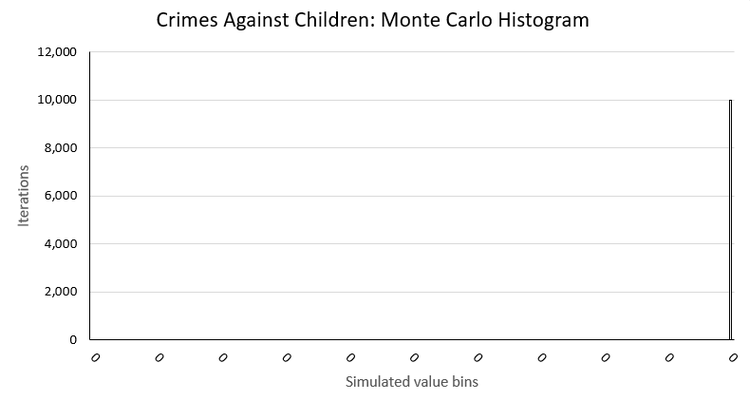
\includegraphics[width=\linewidth]{figures/Screenshot 2026-08-06 085637.png}}}
  \caption{The Monte Carlo simulation determined that there would be no reasonable chance of crimes against children in this sample.  \protect\endnote{\index{sample} sample size was set equivalent to the City of\index{Chattanooga} Chattanooga to determine the per capita rates for each year over data from \index{American Samoa} American Samoa and \index{California} California.  The medians of those rates were used to set 10\% and 90\% \index{confidence interval} confidence intervals with \index{American Samoa} American Samoa and\index{California} California representing low and high \index{cybercrime} cybercrime impact values respectively.}
  \protect\endnote{Monte Carlo Modeling Toolkit authored by Derek E. Brink, CISSP, \url{www.linkedin.com/in/derekbrink}. March 2023.}
  }
  \label{fig:screenshot-montecarlopersdatabreachimpact}
\end{figure}

\begin{figure}[H]
  \centering
  \rotatebox{0}{\scalebox{1}{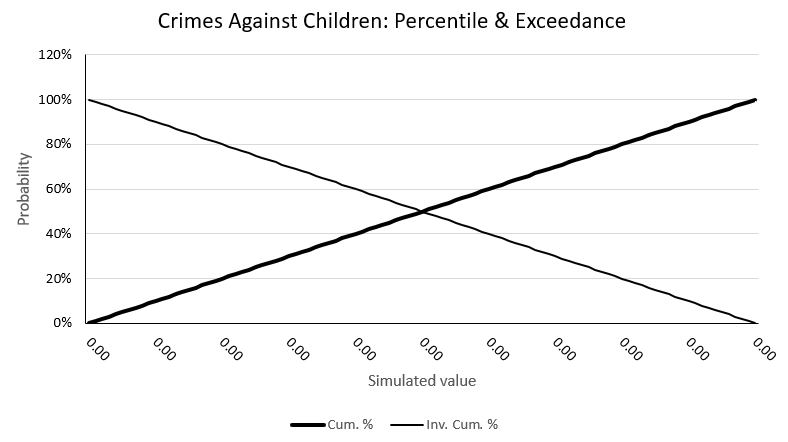
\includegraphics[width=\linewidth]{figures/Screenshot 2026-08-06 090100.png}}}
  \caption{Since the Monte Carlo simulation determined that there would be no reasonable chance of crimes against children in this sample, we can see that there would be no financial impact.  \protect\endnote{\index{sample} sample size was set equivalent to the City of\index{Chattanooga} Chattanooga to determine the per capita rates for each year over data from \index{American Samoa} American Samoa and \index{California} California.  The medians of those rates were used to set 10\% and 90\% \index{confidence interval} confidence intervals with \index{American Samoa} American Samoa and\index{California} California representing low and high \index{cybercrime} cybercrime impact values respectively.}
  \protect\endnote{Monte Carlo Modeling Toolkit authored by Derek E. Brink, CISSP, \url{www.linkedin.com/in/derekbrink}. March 2023.}
  }
  \label{fig:screenshot-montecarlopersdatabreachimpact}
\end{figure}

\subsubsection{Threats to Theft of Data Via Network}
\begin{table}[H]
  \centering
  \caption{Projected In-City Victim Counts, City of\index{Chattanooga} Chattanooga, Theft of Data Via Network}
  \label{tab:chattanoogacrime5}
  \begin{tabular}{@{}
  >{\centering\arraybackslash}p{0.05\linewidth} 
  >{\centering\arraybackslash}p{0.25\linewidth} 
  >{\centering\arraybackslash}p{0.25\linewidth}
  >{\centering\arraybackslash}p{0.25\linewidth}
  >{\centering\arraybackslash}p{0.05\linewidth} }
    \toprule
  Year&\gls{ipr} and Counterfeit&Identify Theft&\gls{bec}&\\

    \midrule
2016&1&7&4&\endnote{original\url{https://www.ic3.gov/Media/PDF/AnnualReport/2016State/StateReport.aspx\#?s=47} current \url{https://www.ic3.gov/AnnualReport/Reports/2016_IC3Report.pdf}}\\
2017&1&8&4&\endnote{original:\url{https://www.ic3.gov/Media/PDF/AnnualReport/2017State/StateReport.aspx\#?s=47} current: \url{https://www.ic3.gov/AnnualReport/Reports/2017_IC3Report.pdf}}\\
2018&0&10&7&\endnote{original:\url{https://www.ic3.gov/Media/PDF/AnnualReport/2018State/StateReport.aspx\#?s=47} current: \url{https://www.ic3.gov/AnnualReport/Reports/2018_IC3Report.pdf}}\\
2019&1&7&8&\endnote{original:\url{https://www.ic3.gov/Media/PDF/AnnualReport/2019State/StateReport.aspx\#?s=47} current: \url{https://www.ic3.gov/AnnualReport/Reports/2019_IC3Report.pdf}}\\
2020&1&10&6&\endnote{original:\url{https://www.ic3.gov/Media/PDF/AnnualReport/2020State/StateReport.aspx\#?s=47} current: \url{https://www.ic3.gov/AnnualReport/Reports/2020_IC3Report.pdf}}\\
2021&1&13&8&\endnote{original:\url{https://www.ic3.gov/Media/PDF/AnnualReport/2021State/StateReport.aspx\#?s=47} current: \url{https://www.ic3.gov/AnnualReport/Reports/2021_IC3Report.pdf}}\\
2022&0&14&10&\endnote{original:\url{https://www.ic3.gov/Media/PDF/AnnualReport/2022State/StateReport.aspx\#?s=47} current: \url{https://www.ic3.gov/AnnualReport/Reports/2022_IC3Report.pdf}}\\

        \bottomrule \end{tabular} 
  \raggedright{Counts deduced from IC3 Victim Complaints for Tennessee adjusted for a per-capita rate and then multiplied by the city's \index{population} population for that year.}
\end{table}

\subsection{Methodology for\index{simulation!Monte Carlo} Monte Carlo Simulations in Excel}
We chose \gls{ic3} crime data from \index{American Samoa} American Samoa to act as our 10\% confidence limit.  We chose data from Californiz to act as our 90\% confidence limit.  We set those limits by looking at seven year spans of crime data and taking the median.  This means we would be likely to have observations above and below the limits, but that the limits themselves would have a basis in observation.  
We input and processed the data as follows:
\begin{itemize}
\item We imported the data from\gls{ic3} crime tables
\item We calculated counts and costs for\index{Chattanooga} Chattanooga, \index{American Samoa} American Samoa, and\index{California} California.
\item We imported a Uniform distribution table from the\index{simulation!Monte Carlo} Monte Carlo Toolkit.
\item We set median summary counts from \index{American Samoa} American Samoa as our 10\% interval.
\item We set median summary counts from\index{California} California as our 90\% interval.
\item We accepted the\index{simulation!Monte Carlo} Monte Carlo percentages and exceedence curves.
\end{itemize}




\section{Analysis}

\subsection{Using Nation or State Data as a Control for Smaller Forecasts}

If we apply unadjusted for\index{sample} sample size counts limited to a one-year basis, we could use a Poisson distribution as shown in Figure \ref{fig:statevent-poissoncontrolsummary}.

\begin{figure}[H]
  \centering

\[
X_{j,i} =
\begin{cases}
M_{j,i} & \text{if victim count} \\
V_{j,i} & \text{if victim impact} \\
S_{j,i} & \text{if suspect count} \\
D_{j,i} & \text{if suspect impact}
\end{cases}
\]

\[
Y_i = \sum_{j=t}^{t+6} X_{j,i}
\]

\[
Y_i \sim \operatorname{Poisson}(\lambda_i \, E_i)
\]

\[
R_i = \frac{Y_i}{E_i}
\]

  \caption{Summary of applying Poisson distribution to counts from nation and state data.}
  \label{fig:statevent-poissoncontrolsummary}
\end{figure}

This would allow us to feed per-state or national data into the forumla and better understand the relationship of our projections to a larger view.  It could help us to understand where our projected\index{sample} sample's forcast would stand against the whole state overall or nationally.  This way, we could use the state and national data as controls for understanding the context of our forecast.

% Empirical rate per year
\begin{figure}[H]
  \centering

\[
r_{j,i} = \frac{Y_{j,i}}{P_j}
\]
  \caption{Empirical rate per year}
  \label{fig:analysis-empiricalrate}
\end{figure}

% Aggregated count and exposure over historical window
\begin{figure}[H]
  \centering
\[
Y_i = \sum_{j=t}^{t+6} Y_{j,i}
\qquad
E_i = \sum_{j=t}^{t+6} P_j
\]
  \caption{Aggregated count and exposure over historical window}
  \label{fig:analysis-aggcountwindow}
\end{figure}

% Directly standardized (weighted mean) rate
\begin{figure}[H]
  \centering
\[
\bar{r}_i = \frac{Y_i}{E_i} = \frac{\displaystyle\sum_{j=t}^{t+6} Y_{j,i}}{\displaystyle\sum_{j=t}^{t+6} P_j}
\]
  \caption{Directly standardized (weighted mean) rate}
  \label{fig:analysis-weightedmeanrate}
\end{figure}

% Poisson model for the aggregated count
\begin{figure}[H]
  \centering
\[
Y_i \sim \operatorname{Poisson}\!\left(\bar{r}_i \cdot E_i\right)
\]
  \caption{Poisson model for the aggregated count}
  \label{fig:analysis-poissonaggcount}
\end{figure}

% Approximate 95\% confidence interval for the rate
\begin{figure}[H]
  \centering
\[
\bar{r}_i \pm 1.96 \sqrt{\frac{\bar{r}_i}{E_i}}
\]
  \caption{Approximate 95\% confidence interval for the rate}
  \label{fig:analysis-95confidencerate}
\end{figure}

% Forecast evaluation: is the forecast within the control band?
\begin{figure}[H]
  \centering
\[
\hat{R}_i \in \left[
  \bar{r}_i - 1.96\sqrt{\frac{\bar{r}_i}{E_i}},\;
  \bar{r}_i + 1.96\sqrt{\frac{\bar{r}_i}{E_i}}
\right]
\]
  \caption{Forecast evaluation: is the forecast within the control band?}
  \label{fig:analysis-forecasteval}
\end{figure}


%----------------------------------------------------------------------------------------
\section{Discussion}

\subsection{Why Some Categories Might Be Lower}
As we look over some of our generated statistics, we can see that sometimes our expectations were defied.  Why, for example, are some of the categories so low in likelihood?  At our level of access to the data from \gls{ic3}, we don't know more of the background details that might point directly to a cause for that.  Perhaps law enforcement gets better insight; but, we have to make do with what we have.  Let's consider some of the categories and suppose, arbitrarily and based on our experience, why some of the figures might be the way they are.

First, we have the overall effect of the convenience sample.  As we mentioned earlier, these reports are based on voluntary disclosures to \gls{us} \gls{fbi} \gls{ic3}.  That means that we could see lower numbers in areas where victims were not motivated to disclose.  

Potential victims could also have successful mitigation efforts in place.  For example, we see lower corporate data breaches than personal data breaches.  Persumably, corporations have security departments that can help them to operate enterprise grade defensive tools when individual people cannot.  Also, we see low counts in malware and ransomware when those categories are often in the news.  It could be that conventional antivirus scanners and endpoint defenses do a good job of neutralizing known malware threats.  If a large number of antivirus users are being protected successfully, then we might have a small number of victimization claims to the \gls{ic3}. 


\subsection{Crimes Against Children and Complaints}

\subsection{Business Email Compromise Versus Ransomware}
A long standing pattern of expectation is that a user will be phished, malware will be deployed on their machine, and then a company will face a ransomware attack.  Besides this, we see a business email compromise category.  If \gls{bec} is a precedent attack, then why aren't its numbers higher?

One of the reasons could be the ramifications of the attacks and their flow into later reporting classifications.  \gls{bec}
attacks could also flow in other directions like credential stuffing attacks or passive surveillance. In credential stuffing, the known business email address might be reused in later follow-on attacks to other systems.  If an attacker chooses a victim that's a key individual in the company, then passive surveillance of the email account might yield valuable information.  Several 10K reports cite top executives getting their accounts monitored through what looks like a combination of passive surviellance and \gls{bec}.

These hint in the numbers can suggest to us an illustration that the overall classification of an attack may not offer direct insight on all of the tactics and techniques that concern us as defenders.  This shouldn't surprise us; we see plenty of evidence in MITRE ATT\&CK, for instance, that most \gls{apt}s use several layers of \gls{ttps}.

\printchapterendnotes



%----------------------------------------------------------------------------------------
%	CHAPTER
%----------------------------------------------------------------------------------------

\chapter{Amnesiac Systems in FreeBSD}

%\begin{lstlisting}[language=KRC,caption={Hello world}]
%#include <stdio.h>
%
%int main(void) {
%    printf("hello, world\n");
%    return 0;
%}
%\end{lstlisting}





		\noindent In this technical note, we explore \index{configuration}\gls{configuration}s of the \index{FreeBSD}FreeBSD \index{operating system}\gls{operating system}.  With a goal of creating an \index{amnesiac}\gls{amnesiac} system that keeps the \index{operating system}\gls{operating system} separate from working storage drives, we experiment with various \index{configuration}\gls{configuration}s.  We demonstrate the planning of drive index{configuration}\gls{configuration} \index{coding}\gls{coding} and the reasoning behind the choices.  First, we code a system that uses the \index{operating system}\gls{operating system} on the storage drive discs.  Then we evolve the plan into using a live cd\index{live CD} for \index{operating system}\gls{operating system} use with drives that are connected to the \gls{immutable system} in \gls{ram} via \gls{configuration} code.  Using an \index{amensiac}amensiac system like this, we would be able to reset the \index{operating system}\gls{operating system} to a known immutable state with every startup.  The drives could be disconnected and reattached to other systems for various purposes.  Throughout, we cover specific commands for drive and \index{operating system}\gls{operating system} management and operation.

\section{Introduction}
\subsection{Background and Content}
In order to maintain persistence, download files, or interact with a file system, attackers need to be able to write to a system.  Many active attack techniques require some kind of writing action as a precedent for execution.  Based on our limited penetration testing and attack experience, we identified 60 Enterprise Technique groups in MITRE ATT\&CK \endnote{MITRE. "Techniques - Enterprise | MITRE ATT\&CK®." Attack.Mitre.Org, 2023, \url{https://attack.mitre.org/techniques/enterprise/}. Accessed 13 July 2026.} that could be thwarted by removing an attacker's ability to write.  This listing is not comprehensive or absolute; we reviewed these technique categories and recognized that at least a naive attempt to carry out those techniques might involve writing to a file or process.  We ignored more passive reconaissance techniques and those that would be executed outside of the target system itself.  Still, we were able to generate a formidable list of attack techniques that would at least be hampered by an operating system that was designed to be immutable.  

We cover our listing of these MITRE ATT\&CK techniques in Tables \ref{tab:mitrewrite1}, \ref{tab:mitrewrite2}, \ref{tab:mitrewrite3}, \ref{tab:mitrewrite4}, \ref{tab:mitrewrite5}, and \ref{tab:mitrewrite6}.  As we review the list, we can see how some might fall into the trap of thinking such a system was invincible or "hack proof".  Our past experience with attack and defense warns us to accept these extensive defenses as tentative.  An ingenious attacker might find a way to carry out these techniques without meeting our preconceived ideas that they require writing or that our chosen forms of immutability would protect against that writing.  Nonetheless, the lengthy list of major groups of techniques and their longer list of subtechniques implies that immutability in the right ways can serve as a provocative and solid form of defense.




\begin{table}
  \centering
  \caption{MITRE ATT\&CK Techniques Require Writing}
  \label{tab:mitrewrite1}
  \begin{tabular}{@{}p{0.30\linewidth} p{0.70\linewidth}}
    \toprule
    Technique Group & Concept \\
    \midrule
Create Account &"Adversaries may create an account to maintain access to victim systems."\endnote{MITRE ATT\&CK. “Create Account, Technique T1136 - Enterprise | MITRE ATT\&CK®." Attack.Mitre.Org, 14 Dec. 2017, \url{https://attack.mitre.org/techniques/T1136/}. Accessed 13 July 2026.}\\
Create or Modify System Process &"Adversaries may create or modify system-level processes to repeatedly execute malicious payloads as part of persistence."\endnote{“Create or Modify System Process, Technique T1543 - Enterprise | MITRE ATT\&CK®." Attack.Mitre.Org, \url{https://attack.mitre.org/techniques/T1543/}. Accessed 13 July 2026.}\\
Data Destruction &"Adversaries may destroy data and files on specific systems or in large numbers on a network to interrupt availability to systems, services, and network resources. "\endnote{“Data Destruction, Technique T1485 - Enterprise | MITRE ATT\&CK®." Attack.Mitre.Org, \url{https://attack.mitre.org/techniques/T1485/}. Accessed 13 July 2026.}\\
Data Encoding &"Adversaries may encode data to make the content of command and control traffic more difficult to detect."\endnote{“Data Encoding, Technique T1132 - Enterprise | MITRE ATT\&CK®." Attack.Mitre.Org, \url{https://attack.mitre.org/techniques/T1132/}. Accessed 13 July 2026.}\\
Data Manipulation &"Adversaries may insert, delete, or manipulate data in order to influence external outcomes or hide activity, thus threatening the integrity of the data."\endnote{---. “Data Manipulation, Technique T1565 - Enterprise | MITRE ATT\&CK®." Attack.Mitre.Org, 2 Mar. 2020, \url{https://attack.mitre.org/techniques/T1565/}. Accessed 13 July 2026.}\\
Data Obfuscation &"Adversaries may obfuscate command and control traffic to make it more difficult to detect."\endnote{“Data Obfuscation, Technique T1001 - Enterprise | MITRE ATT\&CK®." Attack.Mitre.Org, \url{https://attack.mitre.org/techniques/T1001/}. Accessed 13 July 2026.}\\
Data Staged &"Adversaries may stage collected data in a central location or directory prior to Exfiltration."\endnote{“Data Staged, Technique T1074 - Enterprise | MITRE ATT\&CK®." Attack.Mitre.Org, \url{https://attack.mitre.org/techniques/T1074/}. Accessed 13 July 2026.}\\
Defacement  &"Adversaries may modify visual content available internally or externally to an enterprise network, thus affecting the integrity of the original content."\endnote{“Defacement, Technique T1491 - Enterprise | MITRE ATT\&CK®." Attack.Mitre.Org, \url{https://attack.mitre.org/techniques/T1491/}. Accessed 13 July 2026.}\\
Deploy Container &"Adversaries may deploy a container into an environment to facilitate execution or evade defenses."\endnote{“Deploy Container, Technique T1610 - Enterprise | MITRE ATT\&CK®." Attack.Mitre.Org, \url{https://attack.mitre.org/techniques/T1610/}. Accessed 13 July 2026.}\\
Develop Capabilities &"Adversaries may develop capabilities that can be used during targeting."\endnote{“Develop Capabilities, Technique T1587 - Enterprise | MITRE ATT\&CK®." Attack.Mitre.Org, \url{https://attack.mitre.org/techniques/T1587/}. Accessed 13 July 2026.}\\

\bottomrule \end{tabular} \end{table}
\begin{table}
  \centering
  \caption{MITRE ATT\&CK Techniques Require Writing}
  \label{tab:mitrewrite2}
  \begin{tabular}{@{}p{0.40\linewidth} p{0.60\linewidth}}
    \toprule
    Technique Group & Concept \\
    \midrule
Disable or Modify System Firewall &"Adversaries may disable or modify host-based or network firewalls to impair defensive mechanisms and enable further action."\endnote{“Disable or Modify System Firewall, Technique T1686 - Enterprise | MITRE ATT\&CK®." Mitre.Org, 2026, \url{https://attack.mitre.org/techniques/T1686/}. Accessed 13 July 2026.}\\
Disable or Modify Tools &"Adversaries may disable, degrade, or tamper with security tools or applications (e.g., endpoint detection and response (EDR) tools, intrusion detection systems (IDS), antivirus, logging agents, sensors, etc.) to impair or reduce visibility of defensive capabilities. "\endnote{“Disable or Modify Tools, Technique T1685 - Enterprise | MITRE ATT\&CK®." Mitre.Org, 2026, \url{https://attack.mitre.org/techniques/T1685/}. Accessed 13 July 2026.}\\
Disk Wipe &"Adversaries may impair the availability of systems and data by destroying, corrupting, or overwriting data."\endnote{“Disk Wipe, Technique T1561 - Enterprise | MITRE ATT\&CK®." Mitre.Org, 2026, \url{https://attack.mitre.org/techniques/T1561/}. Accessed 13 July 2026.}\\
Domain or Tenant Policy Modification &"Adversaries may modify the configuration settings of a domain or identity tenant to evade defenses and/or escalate privileges."\endnote{“Domain or Tenant Policy Modification, Technique T1484 - Enterprise | MITRE ATT\&CK®." Mitre.Org, 2026, \url{https://attack.mitre.org/techniques/T1484/}. Accessed 13 July 2026.}\\
Escape to Host &"Adversaries may break out of a container to gain access to the underlying host."\endnote{“Escape to Host, Technique T1611 - Enterprise | MITRE ATT\&CK®." Mitre.Org, 2026, \url{https://attack.mitre.org/techniques/T1611/}. Accessed 13 July 2026.}\\Event Triggered Execution &"Adversaries may establish persistence and/or elevate privileges using system mechanisms that trigger execution based on specific events."\endnote{“Event Triggered Execution, Technique T1546 - Enterprise | MITRE ATT\&CK®." Mitre.Org, 2026, \url{https://attack.mitre.org/techniques/T1546/}. Accessed 13 July 2026.}\\
Exclusive Control &"Adversaries who successfully compromise a system may attempt to maintain persistence by "closing the door" behind them – in other words, by preventing other threat actors from initially accessing or maintaining a foothold on the same system."\endnote{“Exclusive Control, Technique T1668 - Enterprise | MITRE ATT\&CK®." Mitre.Org, 2026, \url{https://attack.mitre.org/techniques/T1668/}. Accessed 13 July 2026.}\\
Execution Guardrails  &"Adversaries may use execution guardrails to constrain execution to specific environments."\endnote{“Execution Guardrails, Technique T1480 - Enterprise | MITRE ATT\&CK®." Mitre.Org, 2026, \url{https://attack.mitre.org/techniques/T1480/}. Accessed 13 July 2026.}\\
Exfiltration Over Physical Medium &"Adversaries may exfiltrate data using removable media."\endnote{“Exfiltration Over Physical Medium, Technique T1052 - Enterprise | MITRE ATT\&CK®." Mitre.Org, 2026, \url{https://attack.mitre.org/techniques/T1052/}. Accessed 13 July 2026.}\\
File and Directory Permissions Modification  &"Adversaries may modify file and directory permissions or attributes to evade access control restrictions."\endnote{“File and Directory Permissions Modification, Technique T1222 - Enterprise | MITRE ATT\&CK®." Mitre.Org, 2026, \url{https://attack.mitre.org/techniques/T1222/}. Accessed 13 July 2026.}\\


\bottomrule \end{tabular} \end{table}
\begin{table}
  \centering
  \caption{MITRE ATT\&CK Techniques Require Writing}
  \label{tab:mitrewrite3}
  \begin{tabular}{@{}p{0.40\linewidth} p{0.60\linewidth}}
    \toprule
    Technique Group & Concept \\
    \midrule
Firmware Corruption &"Adversaries may use malicious code embedded in firmware to maintain persistence or disrupt systems."\endnote{“Firmware Corruption, Technique T1495 - Enterprise | MITRE ATT\&CK®." Mitre.Org, 2026, \url{https://attack.mitre.org/techniques/T1495/}. Accessed 13 July 2026.}\\
Hide Artifacts &"Adversaries may abuse functionality to hide artifacts from the user or security tools."\endnote{“Hide Artifacts, Technique T1564 - Enterprise | MITRE ATT\&CK®." Mitre.Org, 2026, \url{https://attack.mitre.org/techniques/T1564/}. Accessed 13 July 2026.}\\
Hijack Execution Flow &"Adversaries may execute their own malicious payloads by hijacking the way operating systems load programs."\endnote{“Hijack Execution Flow, Technique T1574 - Enterprise | MITRE ATT\&CK®." Mitre.Org, 2026, \url{https://attack.mitre.org/techniques/T1574/}. Accessed 13 July 2026.}\\
Implant Internal Image &"Adversaries may implant malicious software into software images to establish persistence."\endnote{“Implant Internal Image, Technique T1525 - Enterprise | MITRE ATT\&CK®." Mitre.Org, 2026, \url{https://attack.mitre.org/techniques/T1525/}. Accessed 13 July 2026.}\\
Indicator Removal &"Adversaries may delete or modify artifacts generated on a system to remove evidence of their presence."\endnote{“Indicator Removal, Technique T1070 - Enterprise | MITRE ATT\&CK®." Mitre.Org, 2026, \url{https://attack.mitre.org/techniques/T1070/}. Accessed 13 July 2026.}\\
Ingress Tool Transfer &"Adversaries may transfer tools or other files from an external system into a compromised environment."\endnote{“Ingress Tool Transfer, Technique T1105 - Enterprise | MITRE ATT\&CK®." Mitre.Org, 2026, \url{https://attack.mitre.org/techniques/T1105/}. Accessed 13 July 2026.}\\
Inhibit System Recovery &"Adversaries may interrupt availability of system and network resources by inhibiting system recovery."\endnote{“Inhibit System Recovery, Technique T1490 - Enterprise | MITRE ATT\&CK®." Mitre.Org, 2026, \url{https://attack.mitre.org/techniques/T1490/}. Accessed 13 July 2026.}\\
Lateral Tool Transfer  &"Adversaries may transfer tools or other files between systems in a compromised environment."\endnote{“Lateral Tool Transfer, Technique T1570 - Enterprise | MITRE ATT\&CK®." Mitre.Org, 2026, \url{https://attack.mitre.org/techniques/T1570/}. Accessed 13 July 2026.}\\
Masquerading &"Adversaries may attempt to manipulate features of their artifacts to make them appear legitimate or benign to users and/or security tools."\endnote{“Masquerading, Technique T1036 - Enterprise | MITRE ATT\&CK®." Mitre.Org, 2026, \url{https://attack.mitre.org/techniques/T1036/}. Accessed 13 July 2026.}\\
Modify Authentication Process &"Adversaries may modify authentication processes and mechanisms to bypass or weaken authentication requirements."\endnote{“Modify Authentication Process, Technique T1556 - Enterprise | MITRE ATT\&CK®." Mitre.Org, 2026, \url{https://attack.mitre.org/techniques/T1556/}. Accessed 13 July 2026.}\\
\bottomrule \end{tabular} \end{table}
\begin{table}
  \centering
  \caption{MITRE ATT\&CK Techniques Require Writing}
  \label{tab:mitrewrite4}
  \begin{tabular}{@{}p{0.40\linewidth} p{0.60\linewidth}}
    \toprule
    Technique Group & Concept \\
    \midrule
Modify Cloud Compute Infrastructure  &"Adversaries may create, modify, or delete cloud resources to achieve their objectives."\endnote{“Modify Cloud Compute Infrastructure, Technique T1578 - Enterprise | MITRE ATT\&CK®." Mitre.Org, 2026, \url{https://attack.mitre.org/techniques/T1578/}. Accessed 13 July 2026.}\\
Modify Cloud Resource Hierarchy &"Adversaries may attempt to modify hierarchical structures in infrastructure-as-a-service (IaaS) environments in order to evade defenses."\endnote{“Modify Cloud Resource Hierarchy, Technique T1666 - Enterprise | MITRE ATT\&CK®." Mitre.Org, 2026, \url{https://attack.mitre.org/techniques/T1666/}. Accessed 13 July 2026.}\\
Modify Registry &"Adversaries may interact with the Windows Registry to hide configuration information, modify system settings, or remove information as part of their attack."\endnote{“Modify Registry, Technique T1112 - Enterprise | MITRE ATT\&CK®." Mitre.Org, 2026, \url{https://attack.mitre.org/techniques/T1112/}. Accessed 13 July 2026.}\\
Modify System Image &"Adversaries may modify the configuration of network devices to maintain access, modify traffic flows, or disrupt services."\endnote{“Modify System Image, Technique T1601 - Enterprise | MITRE ATT\&CK®." Mitre.Org, 2026, \url{https://attack.mitre.org/techniques/T1601/}. Accessed 13 July 2026.}\\
Multi-Stage Channels &"Adversaries may use multiple command and control channels to communicate with compromised systems."\endnote{“Multi-Stage Channels, Technique T1104 - Enterprise | MITRE ATT\&CK®." Mitre.Org, 2026, \url{https://attack.mitre.org/techniques/T1104/}. Accessed 13 July 2026.}\\
Obfuscated Files or Information &"Adversaries may obfuscate their malicious code, configuration files, or other artifacts to make detection and analysis more difficult."\endnote{“Obfuscated Files or Information, Technique T1027 - Enterprise | MITRE ATT\&CK®." Mitre.Org, 2026, \url{https://attack.mitre.org/techniques/T1027/}. Accessed 13 July 2026.}\\
OS Credential Dumping &"Adversaries may attempt to dump credentials to obtain account information that can be used to access systems and services."\endnote{“OS Credential Dumping, Technique T1003 - Enterprise | MITRE ATT\&CK®." Mitre.Org, 2026, \url{https://attack.mitre.org/techniques/T1003/}. Accessed 13 July 2026.}\\
Plist File Modification &"Adversaries may modify browser extensions to execute malicious code or collect information from a victim's browser."\endnote{“Plist File Modification, Technique T1647 - Enterprise | MITRE ATT\&CK®." Mitre.Org, 2026, \url{https://attack.mitre.org/techniques/T1647/}. Accessed 13 July 2026.}\\
Poisoned Pipeline Execution &"Adversaries may manipulate continuous integration / continuous development (CI/CD) processes by injecting malicious code into the build process. "\endnote{“Poisoned Pipeline Execution, Technique T1677 - Enterprise | MITRE ATT\&CK®." Mitre.Org, 2026, \url{https://attack.mitre.org/techniques/T1677/}. Accessed 13 July 2026.}\\
Power Settings &"Adversaries may use virtualization and containerization technologies to create or maintain access to compromised environments."\endnote{“Power Settings, Technique T1653 - Enterprise | MITRE ATT\&CK®." Mitre.Org, 2026, \url{https://attack.mitre.org/techniques/T1653/}. Accessed 13 July 2026.}\\

\bottomrule \end{tabular} \end{table}

\begin{table}
  \centering
  \caption{MITRE ATT\&CK Techniques Require Writing}
  \label{tab:mitrewrite5}
  \begin{tabular}{@{}p{0.40\linewidth} p{0.60\linewidth}}
    \toprule
    Technique Group & Concept \\
    \midrule
Pre-OS Boot  &"Adversaries may abuse Pre-OS Boot mechanisms as a way to establish persistence on a system."\endnote{“Pre-OS Boot, Technique T1542 - Enterprise | MITRE ATT\&CK®." Mitre.Org, 2026, \url{https://attack.mitre.org/techniques/T1542/}. Accessed 13 July 2026.}\\
Prevent Command History Logging &"Adversaries may impair command history logging to hide commands they run on a compromised system"\endnote{“Prevent Command History Logging, Technique T1690 - Enterprise | MITRE ATT\&CK®." Mitre.Org, 2026, \url{https://attack.mitre.org/techniques/T1690/}. Accessed 13 July 2026.}\\
Process Injection &"Adversaries may inject code into processes in order to evade process-based defenses as well as possibly elevate privileges."\endnote{“Process Injection, Technique T1055 - Enterprise | MITRE ATT\&CK®." Mitre.Org, 2026, \url{https://attack.mitre.org/techniques/T1055/}. Accessed 13 July 2026.}\\
Protocol Tunneling &"Adversaries may use protocol tunneling to hide network communications through existing protocols or services."\endnote{“Protocol Tunneling, Technique T1572 - Enterprise | MITRE ATT\&CK®." Mitre.Org, 2026, \url{https://attack.mitre.org/techniques/T1572/}. Accessed 13 July 2026.}\\
Proxy &"Adversaries may use a connection proxy to direct network traffic between systems or act as an intermediary for network communications."\endnote{“Proxy, Technique T1090 - Enterprise | MITRE ATT\&CK®." Mitre.Org, 2026, \url{https://attack.mitre.org/techniques/T1090/}. Accessed 13 July 2026.}\\Reflective Code Loading &"Adversaries may reflectively load code into a process in order to conceal the execution of malicious payloads."\endnote{“Reflective Code Loading, Technique T1620 - Enterprise | MITRE ATT\&CK®." Mitre.Org, 2026, \url{https://attack.mitre.org/techniques/T1620/}. Accessed 13 July 2026.}\\
Remote Access Tools &"An adversary may use legitimate remote access tools to establish an interactive command and control channel within a network."\endnote{“Remote Access Tools, Technique T1219 - Enterprise | MITRE ATT\&CK®." Mitre.Org, 2026, \url{https://attack.mitre.org/techniques/T1219/}. Accessed 13 July 2026.}\\
Rogue Domain Controller &"Adversaries may register a rogue Domain Controller to enable manipulation of Active Directory data."\endnote{“Rogue Domain Controller, Technique T1207 - Enterprise | MITRE ATT\&CK®." Mitre.Org, 2026, \url{https://attack.mitre.org/techniques/T1207/}. Accessed 13 July 2026.}\\
Rootkit &"Adversaries may use rootkits to hide the presence of programs, files, network connections, services, drivers, and other system components."\endnote{“Rootkit, Technique T1014 - Enterprise | MITRE ATT\&CK®." Mitre.Org, 2026, \url{https://attack.mitre.org/techniques/T1014/}. Accessed 13 July 2026.}\\
Scheduled Task/Job &"Adversaries may abuse task scheduling functionality to facilitate initial or recurring execution of malicious code."\endnote{“Scheduled Task/Job, Technique T1053 - Enterprise | MITRE ATT\&CK®." Mitre.Org, 2026, \url{https://attack.mitre.org/techniques/T1053/}. Accessed 13 July 2026.}\\

\bottomrule \end{tabular} 
\end{table}

\begin{table}
  \centering
  \caption{MITRE ATT\&CK Techniques Require Writing}
  \label{tab:mitrewrite6}
  \begin{tabular}{@{}p{0.40\linewidth} p{0.60\linewidth}}
    \toprule
    Technique Group & Concept \\
    \midrule
Scheduled Transfer &"Adversaries may attempt to take screen captures of the desktop to gather information over the course of an operation."\endnote{“Scheduled Transfer, Technique T1029 - Enterprise | MITRE ATT\&CK®." Mitre.Org, 2026, \url{https://attack.mitre.org/techniques/T1029/}. Accessed 13 July 2026.}\\    
Screen Capture &"Adversaries may abuse legitimate extensible development features of servers to establish persistent access to systems."\endnote{“Screen Capture, Technique T1113 - Enterprise | MITRE ATT\&CK®." Mitre.Org, 2026, \url{https://attack.mitre.org/techniques/T1113/}. Accessed 13 July 2026.}\\    
Server Software Component &"Adversaries may gain access to and use centralized software suites installed within an enterprise to execute commands and move laterally through the network."\endnote{“Server Software Component, Technique T1505 - Enterprise | MITRE ATT\&CK®." Mitre.Org, 2026, \url{https://attack.mitre.org/techniques/T1505/}. Accessed 13 July 2026.}\\
Software Deployment Tools &"Adversaries may upload, install, or otherwise set up capabilities that can be used during targeting."\endnote{“Software Deployment Tools, Technique T1072 - Enterprise | MITRE ATT\&CK®." Mitre.Org, 2026, \url{https://attack.mitre.org/techniques/T1072/}. Accessed 13 July 2026.}\\
Stage Capabilities &"Adversaries may use shared content to move malicious files or code between systems."\endnote{“Stage Capabilities, Technique T1608 - Enterprise | MITRE ATT\&CK®." Mitre.Org, 2026, \url{https://attack.mitre.org/techniques/T1608/}. Accessed 13 July 2026.}\\
Taint Shared Content &"Adversaries may create or modify references in user document templates to conceal malicious code or force authentication attempts."\endnote{“Taint Shared Content, Technique T1080 - Enterprise | MITRE ATT\&CK®." Mitre.Org, 2026, \url{https://attack.mitre.org/techniques/T1080/}. Accessed 13 July 2026.}\\
Template Injection &"Adversaries may use traffic signaling to hide open ports or other malicious functionality used for persistence or command and control."\endnote{“Template Injection, Technique T1221 - Enterprise | MITRE ATT\&CK®." Mitre.Org, 2026, \url{https://attack.mitre.org/techniques/T1221/}. Accessed 13 July 2026.}\\
Traffic Signaling &"Adversaries may compromise a network device's encryption capability in order to bypass encryption that would otherwise protect data communications."\endnote{“Traffic Signaling, Technique T1205 - Enterprise | MITRE ATT\&CK®." Mitre.Org, 2026, \url{https://attack.mitre.org/techniques/T1205/}. Accessed 13 July 2026.}\\
Weaken Encryption &"Adversaries may bypass application control and obscure execution of code by embedding scripts inside XSL files."\endnote{“Weaken Encryption, Technique T1600 - Enterprise | MITRE ATT\&CK®." Mitre.Org, 2026, \url{https://attack.mitre.org/techniques/T1600/}. Accessed 13 July 2026.}\\
XSL Script Processing &"Adversaries may bypass application control and obscure execution of code by embedding scripts inside XSL files."\endnote{“XSL Script Processing, Technique T1220 - Enterprise | MITRE ATT\&CK®." Mitre.Org, 2026, \url{https://attack.mitre.org/techniques/T1220/}. Accessed 13 July 2026.}\\
\bottomrule \end{tabular} 
\end{table}
\subsection{Problem Statement}


Our goal is to keep the core services and operating system stable and immutable through physical security controls.  This will allow the system to resist common attacks such as the encryption of files from ransomware and persistent account takeovers.  

\subsection{Project Objectives}

Our system, hostname Blondie, set an example for amnesiac system implementation and design with FreeBSD.  We hope that this example system will raise awareness and set patterns that will allow others to gain some of the same risk controls in their systems.

\subsection{Scope of Work}
\subsubsection{Hypothesis:  H1}
\begin{quotation}\raggedright Attackers cannot destructively interact with systems without writing to them.\end{quotation}

Some reflection on "cannot" may lead us into conflict with this hypothesis; so, let's consider carefully what we mean.  At some point in the kill chain, if an attacker wants to stop being passive and start being active and destructive, then they must somehow modify a file on the target system or write a file to the target system.  That file could be in \gls{ram}; it could be in a temporary directory; it could already exist.  Not all attacks require this behavior, but many do.  With some imprecision we assert that attackers need to write to destroy.

ingress tool transfer  MITRE ATT\&CK
\subsubsection{Hypothesis:  H2}
\begin{quotation}\raggedright An immutable operating system will be more resistant to destructive attack.\end{quotation}

\subsubsection{Hypothesis:  H3}
\begin{quotation}\raggedright An immutable operating system will promote system integrity.\end{quotation}

With ransomware as a dominant contemporary threat, integrity of the CIA triad rises to the forefront of defensive needs.  
\subsubsection{Hypothesis:  H4}
\begin{quotation}\raggedright An immutable operating system will promote rapid recovery.\end{quotation}

With core components and configurations unchanged, an immutable system restarted after an attack will experience a more rapid recovery.
\subsection{Variables}

\subsubsection{Non-Adversarial Threats}
\begin{itemize}
	\item Hardware limitations
	\item Coding and configuration errors
	\item Physical deficiencies 
	\item Disasters
\end{itemize}

\subsubsection{Adversarial Threats}
\begin{itemize}
	\item Ransomware
	\item Network attacks
	\item Physical attacks 
	\item Non-malicious insider threats
\end{itemize}

\subsection{Assumptions, Risks, and Limitations}
\subsubsection{Assumptions}
\begin{itemize}
	\item Sufficient time and control for power up, power down, and maintenance operations
	\item Direct control of server stack allows for optical disc use
	\item No migration of an existing commercial stack
	\item No commercial pressure for business performance or profit
\end{itemize}
\subsubsection{Risks}
\begin{itemize}
	\item New procedures require rehearsal
	\item Complex research patterns may cloud known references
	\item Endeavor may be too complex to implement for some teams
	\item Unforseen compatability or integration problems
\end{itemize}
\subsubsection{Limitations}
\begin{itemize}
	\item Increased complexity requires trained personnel
	\item Untaught patterns will require time to learn through experimentation
	\item No known defense against zero day vulnerabilities in the OS
	\item Size constraints on optical discs may limit immutable segment of system
\end{itemize}

\subsection{Significance of the Project}

\section{Literature Review}
\subsection{Overview of Existing Solutions or Approaches}

\subsubsection{Immutability as a Constraining Concept}
We wanted to better understand immutability as an idea.  We came across an article ("Immutability as an Operational Constraint Rather Than a
Security Feature")\endnote{Vppalapati, Mallikarjun. “Immutability as an Operational Constraint rather than a Security Feature.” International Journal of Artificial Intelligence, Data Science, and Machine Learning, vol. 3, no. 2, 30 June 2022, pp. 176–184, \url{https://doi.org/10.63282/3050-9262.ijaidsml-v3i2p119}. Accessed 21 June 2026.}  that pointed out that immutability can be a limiting factor.  The author warned, "By just making something immutable you haven't necessarily made it safe; what you have effectively done is taken away the possibility of alteration and replaced it with a new operational reality: correction must happen through additional writes, and recovery must happen through reconciliation rather than repair"\endnote{Vppalapati, Mallikarjun. “Immutability as an Operational Constraint rather than a Security Feature.” International Journal of Artificial Intelligence, Data Science, and Machine Learning, vol. 3, no. 2, 30 June 2022, pp. 176–184, \url{https://doi.org/10.63282/3050-9262.ijaidsml-v3i2p119}. Accessed 21 June 2026.}  

In this approach, the entire system was assumed to be an immutable system.  This helped us to realize what a benefit it was to not make the entire system immutable.  Our original intention was to have centralized, core, aspects of the operating system be immutable; other parts of the system could be changed within the rules and limits set by the OS.  

Still, those changeable parts might have logging and monitoring activities, such as database snapshots set up in a way that allowed these cautions about immutability to contribute to our planning.  Mallikarjun Vppalapati pointed out problems that could be had when records of on-system actions became immutable.  Suppose a log or record was contaminated with malware or privacy information that needed to be forgotten under \index{GDPR!Right to be Forgotten}\gls{gdpr}.  Administrators might need to undertake complicated edits to allow future auditors to bypass data that should not be considered.  Vppalapati outlined a situation in which a simple programmatic error needed an elaborate and complicated fix because simple overwrites were not available.\endnote{Vppalapati, Mallikarjun. “Immutability as an Operational Constraint rather than a Security Feature.” International Journal of Artificial Intelligence, Data Science, and Machine Learning, vol. 3, no. 2, 30 June 2022, pp. 176–184, \url{https://doi.org/10.63282/3050-9262.ijaidsml-v3i2p119}. Accessed 21 June 2026.}

Vppalapati described three kinds of immutability:  hard, soft, and operational.
"\index{immutability!hard}\Gls{hard immutability} describes a state of being unchangeable where changes are so heavily protected by technical mechanisms
and therefore practically infeasible the alteration process is therefore practically impossible."\endnote{Vppalapati, Mallikarjun. “Immutability as an Operational Constraint rather than a Security Feature.” International Journal of Artificial Intelligence, Data Science, and Machine Learning, vol. 3, no. 2, 30 June 2022, pp. 176–184, \url{https://doi.org/10.63282/3050-9262.ijaidsml-v3i2p119}. Accessed 21 June 2026.}  "\index{immutability!soft}\Gls{soft immutability}...can be reverted by using privileged credentials."\endnote{Vppalapati, Mallikarjun. “Immutability as an Operational Constraint rather than a Security Feature.” International Journal of Artificial Intelligence, Data Science, and Machine Learning, vol. 3, no. 2, 30 June 2022, pp. 176–184, \url{https://doi.org/10.63282/3050-9262.ijaidsml-v3i2p119}. Accessed 21 June 2026.}  "\index{immutability!operational}\Gls{operational immutability} implies the lack of changes without the use of technology"\endnote{Vppalapati, Mallikarjun. “Immutability as an Operational Constraint rather than a Security Feature.” International Journal of Artificial Intelligence, Data Science, and Machine Learning, vol. 3, no. 2, 30 June 2022, pp. 176–184, \url{https://doi.org/10.63282/3050-9262.ijaidsml-v3i2p119}. Accessed 21 June 2026.}  In our proposed system, we would use hard immutability in the optical read-only recording of the core OS.  We would use operational immutability as a control because we were applying an optical disc that required physical access to the server for alterations.  For example, to change the operating system burned to optical disc, an attacker or operator would need to build a new disc and physically insert it into the system, and then follow our proscribed startup sequence to get the \gls{os} into \gls{ram}.  We would also use soft immutability, in the writing of data to files in attached storage that was not automatically loaded by the system on boot.  

\subsubsection{Immutability Examples in Blockchains}
If there's a technology that has a reputation for immutability, it is the blockchain.  Simply put, the blockchain is a chain of cryptographic records; the starting point for the math used to encrypt each block is based on the previous record; the cummulative effect of the sequence of encryption is that if one record is corrupted or modified, then the break in the logic for decrypting subsequent blocks will reveal the change.  So long as the records in the blockchain are accessible, users can assume that the previous entries have been unmodified.  Blockchain has other characteristics; its records are usually distributed over networks and internets; but, the mathematical sequence of encryption and decryption based on preceding blocks is the source of its logical strength as an immutable record.

Blockchains, being immutable, can run into conflict with one of the more famous requirements for mutability of our time:  \index{GDPR!Right to be Forgotten}\gls{gdpr}'s \gls{rtbf}.   
\endnote{Wolford, Ben. “Everything You Need to Know About the ‘Right to Be Forgotten.’” GDPR.Eu, 5 Nov. 2018, \url{https://gdpr.eu/right-to-be-forgotten/}. Accessed 12 July 2026.}\endnote{GDPR. “Art. 17 GDPR - Right to Erasure (‘Right to Be Forgotten’) - GDPR.Eu.” GDPR.Eu, 14 Nov. 2018, \url{https://gdpr.eu/article-17-right-to-be-forgotten/}. Accessed 12 July 2026.}  One of the components of \gls{gdpr}, Recital 65, says that a person who has their data recorded has the right to request a modification or deletion of that data.  There are some exceptions and provisions for children who get their data recorded, but at its core Recital 65 provides every person in the EU with the legal right to have their records modified.  \endnote{“Recital 65 - Right of Rectification and Erasure.” GDPR.Eu, 14 Nov. 2018, \url{https://gdpr.eu/recital-65-right-of-rectification-and-erasure/}. Accessed 12 July 2026.}  Recital 66 says that a data controller has to inform processors to erase links to or copies of personal data.  This way a request to be forgotten can't just stop with one entity or be restricted to entities that the requestor discovers on their own.  \endnote{“Recital 66 - Right to Be Forgotten.” GDPR.Eu, 14 Nov. 2018, \url{https://gdpr.eu/recital-66-right-to-be-forgotten/}. Accessed 12 July 2026.}  In these laws, we don't see exceptions for immutable systems built-in.  On the contrary, by being left out altogether the responsibility for dealing with these legal conflicts seems to go back on the immutable system owner.  If a system were to operate that was truly immutable, then if that system contained personal data that was to be erased upon a given request:  it might require the destruction of the whole system to bring the operator into legal compliance with \gls{gdpr}.  This might not be as catastrophic as it sounds; perhaps an operator could take a system offline, delete a record, and then completely regenerate the records with the required deletions omitted.  However, multiple such mutations could lead to complexities in system maintenance with multiple required regenerations.  The problem could get further complicated if the system had subsequent sequential modifications.  Altogether, system operators would be cautioned not to store personal data in immutable file structures.  Perhaps we might be further cautioned to keep immutable only what was operationally necessary as a safeguard against future laws or requirements.  As we work through the implementation of our immutable system, we shall see that sometimes the constraints can bring us structure and sometimes the limitations are innovation accellerators.

Blockchains offer an example of Vppalapati's \gls{hard immutability} and \gls{operational immutability}.  The \gls{eu}'s \gls{gdpr} counters with an example of \gls{soft immutability} requirements for certain kinds of data.  We can conclude that most personal data would have to be kept off of the optical discs (and out of any network distributed blockchains).  While most \gls{pii} would not seem to be a part of an operating system, later we'll see that a user's full name is requested by the system as a normal part of user account setup.  We could have a small conflict that leads to an involved repair if we're not careful. 

We found an article which examined the types of problems with blockchains in detail.  The authors classified the problems into four main categories:  

\subsubsection{Immutability Examples in Database Administration}

\subsection{Comparisons of Technologies or Frameworks}
\subsubsection{Immutability and MAC Biba}
\index{mac!biba}\Gls{biba} is a mandatory access control scheme, similar to military multilevel security classifications, but with an emphasis on file integrity. \texttt{mac\_biba} allows for write down and read up; this is the opposite direction from mandatory access control schemes like military security classifications which can write up and read down. \endnote{Martins, Gary R., et al. Implementing Message Systems in Multilevel Secure Environments: Problems and Approaches. Rand, 1982.}
\endnote{Biba, K J, et al. Integrity Considerations for Secure Computer Systems. 1977.} FreeBSD offers \texttt{mac\_biba} as part of its operating system; unfortunately, OpenBSD does not.  \endnote{"Mac\_Biba(4)." Freebsd.Org, 2025, \url{https://man.freebsd.org/cgi/man.cgi?query=mac_biba&sektion=4&apropos=0&manpath=freebsd+15.1-release+and+ports}. Accessed 13 July 2026.}
... compare with diagrams 

% ...
\begin{figure}[htbp]
  \centering
  \rotatebox{0}{\scalebox{1}{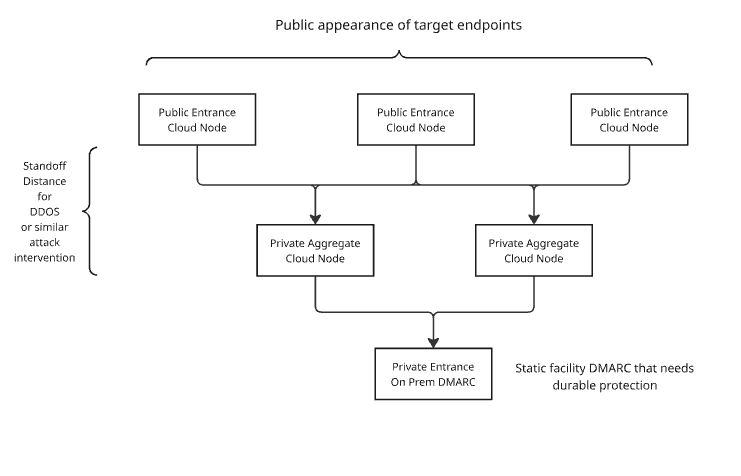
\includegraphics[width=\linewidth]{figures/public to private}}}
  \caption{Your caption}
  \label{fig:your-figure}
\end{figure}

\subsection{Gaps in the Literature}
\section{Methodology}
\subsection{Technical Research Questions}
\subsection{System Architecture and Design}
\subsection{Implementation Plan}
We're starting with a Dell T610 Server.  Made in 2011, this machine is about ten years old.  We purchased this at a government e-waste auction.  She needed some cleanup.  We started on the front lawn, blowing out the dust with a leafblower.  

Most of the time servers from these auctions will have minimal \gls{ram}.  Usually the drives and any good accessories will be stripped out.  Anytime we get a hard drive, from any source, one of the first actions we take is to erase the drives to \gls{us} \gls{nist} 800-88 Purge\index{NIST 800-88!Purge}\endnote{Chandramouli, Ramaswamy. Guidelines for Media Sanitization. 2025, \url{nvlpubs.nist.gov/nistpubs/SpecialPublications/NIST.SP.800-88r2.pdf}, \url{https://doi.org/10.6028/nist.sp.800-88r2}.} with dedicated devices.  That kind of erasing can be done with \index{dd}\texttt{dd} in Kali or \index{FreeBSD}FreeBSD; but, the drive erasers usually have a verification feature that's helpful.  
\subsubsection{Hardware \Gls{configuration}}
This is my favorite computer.  I've named her "Blondie" after Debbie Harry's New Wave band.\endnote{“Blondie | the Official Website of Blondie, Featuring Tour Dates, Presale Ticketing, News, the Official Store and More.” \url{Blondie.net}, 2026, blondie.net/. Accessed 10 June 2026.}

Now, she's configured with:
\begin{itemize}
	\item A DVD RW drive
    	\item A \index{LTO III tape}LTO III\endnote{“LTO Ultrium 3: Product Views | Fujifilm [United States].” Fujifilm.com, 2026, \url{www.fujifilm.com/us/en/business/data-storage/data-storage-media/lto-ultrium-3/product-views}. Accessed 10 June 2026.} tape backup unit
    	\item In her 8 drive bay, we have:
	\begin{itemize}
		\item Two VelociRaptor\endnote{''WD VelociRaptor ® \GLS{sata} Hard Drives'' \url{https://theretroweb.com/storage/documentation/wd6000-velociraptor-68407cb5c0c96653507203.pdf}} 80GB 10000 rpm drives.
		\begin{itemize}
			\item We'll use these in a \Gls{mirror} \gls{configuration} to hold the main OS.
		\end{itemize}
		\item Two refurb 120GB \GLS{ssd}s
		\begin{itemize}
			\item We'll use this in a \Gls{mirror} as ZFS log drives.
			\item They'll help to make writes faster.
		\end{itemize}
		\item Four 500GB hard drives
		\begin{itemize}
			\item We'll use this as a \index{RAIDZ-2}RAIDZ-2 array to hold the \glspl{jail}.
			\item We have some smaller \GLS{sas} drives.
			\item We have some \GLS{sata} drives.
		\end{itemize}
		\end{itemize}
		\item We replaced the one CPU with two Xeon 5550\endnote{Intel® Xeon® Processor 5500 Series an Intelligent Approach to IT Challenges. \url{www.intel.com/content/dam/doc/product-brief/xeon-5500-server-brief.pdf.}} quad cores and added a cooling tower.
		\item We added more \gls{ram}.  Currently, we're at 196GB.
		\item We added some more \gls{nic}s.
		\begin{itemize}
			\item We have four for the jails.
			\item We have two for the OS.
			\item We'll leave the two on the  \gls{motherboard} mostly unused, except for our iDRAC connection.
			\begin{itemize}
				\item iDRAC is a proprietary baseboard controller.  
				\item We could use it to power cycle the machine.
				\item There's a web interface that let's us know about  \gls{motherboard}-related facts.
				\item We cannot give a \index{geli}GELI password through the console in our current setup.
			\end{itemize}	
	\end{itemize}
	\item The server has two 500W power supplies.
\end{itemize}
Because the dual power supplies draw about 500 Watts apiece, this server gets it own circuit.

The drives we're using are older, but we got enough copies of the drives to be able to support backups.  When making physical backups of the drives, it can be helpful to have other volumes of the same model.  So, instead of getting the best available, we planned for the best we could afford at quantity.

The server does not have:
\begin{itemize}
	\item Any type of graphics card or \gls{gpu}
	\item Sound cards or microphone hardware
	\item Wireless networking or Bluetooth.
\end{itemize}
\subsubsection{Intentions:  Paving the Road to Jails}
We'll use the box for development.  It'll be our main development server.  We'll use it with prog\gls{ram}s that we compile on a nearby poudriere package building box.  In those package builds, we have segregated our builds into a pattern of jails that mimic the types of jails that will be needed on most of our computers.  

So, there is a \gls{jail} for functional groups like:  development tools, offensive and defensive security programs, browsers, desktop software, and so on.  \gls{poudriere} jails can be filled with whatever sets of programs we like.  For successful builds, we find its best to keep the jails small.  

There will be three main groups of drives:
\begin{itemize}
	\item an OS \Gls{mirror} pair
	\item a ZFS log \Gls{mirror} pair
	\item a ZFS \index{RAIDZ-2}RAIDZ-2 kit of four drives.
\end{itemize}

The OS pair will hold ideas like:
\begin{itemize}
	\item jail \gls{configuration}
	\item main host networking and \gls{vnet}
	\item host-based user accounts and \gls{configuration}.
\end{itemize}

The ZFS kits will hold disconnected jails.  We'll set up a system of hierarchical jails that provide us with a development environment made up of modular jails that will be the children of an overarching parent.  These jails will communicate with each other and the parent through some custom \gls{vnet}.  We'll do all of our jail scripting, controls, and \gls{configuration} manually.  Likewise, the base ZFS setup will be done with simple scripts.
%------------------------------------------------


\subsubsection{Preparing the Baseboard}

The T610 has a built-in  \gls{raid} card that can't be totally bypassed.  This means that since we'll want ZFS to control the drives as much as possible, we'll need to tell the hardware  \gls{raid} to buzz off.  We won't want hardware  \gls{raid} to participate in the process.  We'll just use the software  \gls{raid} through ZFS.

We can't just unplug the  \gls{raid} card.  We tried that, and it leads to malfunctions on this machine.  So, as a compromise, what we'll tell the machine is that each drive is its own VDEV and it's RAID-0.  We'll end up with as many VDEVs as we have physical drives.  

To prepare for a later step in this process, we'll note the serial number of each drive we load into position, its model number, and its capacity.  We'll need to know that information, and we won't want to be hassled by having to power cycle the machine in the middle of the setup process just to check on those details.

Later on, we'll set VDEVs with ZFS; but, from this point on, we'll basically ignore the  \gls{raid} card's description of these devices as VDEVs.  

With the baseboard prepared, and the BIOS set to allow us to boot from disc, we'll get started with a plain install of \index{FreeBSD}FreeBSD to the first two drives in a \Gls{mirror} \gls{configuration}.

\subsubsection{Incremental Advancement to \Gls{amnesiac} System}
With all of the manual \index{coding}\gls{coding} and \gls{configuration} needed to set up an \gls{amnesiac} system like the one we desired, it was a big change from the normal \gls{bsd} installs we had done for several years.  Our first pass at building an \gls{amnesiac} system decayed into manually scripting a regular \index{operating system}\gls{operating system} installation that had most of the features we desired in the \gls{amnesiac} system.  Both the on-disc OS system and the \gls{amnesiac} system are detailed below.  

\subsubsection{Identifying and Allocating ZFS Drive Qualities}
We need to be able to detect the drives and partitions that we want to work with using geom, \index{gpart}gpart, and zfs commands.  If, for some reason, you can't find those drives, then you need to address that.  While working with this particular computer, I've found that the leading cause of failing to detect a drive goes back to the VDEV assignment in the hardware  \gls{raid}.  If the drive were pulled, this particular  \gls{raid} card will need to have those \gls{configuration} changes addressed.  Often, this means rebooting the machine.  It could be done through the iDRAC baseboard controller in some models; but the one we have here is not configured to do those tasks.

\subsubsection{What are we going to want the ZFS kit to do?  How are we going to use the drives?  How can we wrestle with this new type of \gls{configuration}?}
\begin{table}
  \centering
  \caption{ZFS Concepts and Commands}
  \label{tab:zfsconcepts}
  \begin{tabular}{@{}p{0.30\linewidth} p{0.30\linewidth} p{0.40\linewidth}@{}}
    \toprule
    Topic & Concept & Command phrase example \\
    \midrule
    Disk labels & Use the label to associate the logical with the physical\endnote{Lucas, Michael W, and Allan Jude. FreeBSD Mastery: ZFS. Tilted Windmill Press, 21 May 2015.} &
      \texttt{[Host]-[PositionNumber 0-7]-[Serial\_Number]}\endnote{This pattern of coordinating host computer, bay position, and drive serial number was recommended by Lucas and Jude.  Lucas, Michael W, and Allan Jude. FreeBSD Mastery: ZFS. Tilted Windmill Press, 21 May 2015.}\\
    ZFS Compression & Faster performance: less space\endnote{Lucas, Michael W, and Allan Jude. FreeBSD Mastery: ZFS. Tilted Windmill Press, 21 May 2015.} &
      \texttt{zfs set compress=gzip-6 [DIRECTORY]}\endnote{zfs set shown in:  “Zfs.” Freebsd.org, 2025, \url{man.freebsd.org/cgi/man.cgi?query=zfs&apropos=0&sektion=0&manpath=FreeBSD+14.0-RELEASE&arch=default&format=html}. Accessed 10 June 2026.}  \\
    ZFS \index{zpool!comment}zpool comment& Make a note on the pool\endnote{Lucas, Michael W, and Allan Jude. FreeBSD Mastery: ZFS. Tilted Windmill Press, 21 May 2015.} &
      \texttt{zfs set comment="-"}\endnote{zfs set shown in:  “Zfs.” Freebsd.org, 2025, \url{man.freebsd.org/cgi/man.cgi?query=zfs&apropos=0&sektion=0&manpath=FreeBSD+14.0-RELEASE&arch=default&format=html}. Accessed 10 June 2026.}  \\
    quota\endnote{“Chapter 6 Managing ZFS File Systems (Solaris ZFS Administration Guide).” \url{Docs.oracle.com, docs.oracle.com/cd/E19120-01/open.solaris/817-2271/6mhupg6m3/index.html}.}& Limit growth\endnote{Lucas, Michael W, and Allan Jude. FreeBSD Mastery: ZFS. Tilted Windmill Press, 21 May 2015.} & --- \\
    reservation\endnote{“Chapter 6 Managing ZFS File Systems (Solaris ZFS Administration Guide).” \url{Docs.oracle.com, docs.oracle.com/cd/E19120-01/open.solaris/817-2271/6mhupg6m3/index.html}.} & Set aside space for directory and its children\endnote{Lucas, Michael W, and Allan Jude. FreeBSD Mastery: ZFS. Tilted Windmill Press, 21 May 2015.} & --- \\
    refreservation\endnote{“Chapter 6 Managing ZFS File Systems (Solaris ZFS Administration Guide).” \url{Docs.oracle.com, docs.oracle.com/cd/E19120-01/open.solaris/817-2271/6mhupg6m3/index.html}.} & Set aside space but don't count snapshots and child datasets\endnote{Lucas, Michael W, and Allan Jude. FreeBSD Mastery: ZFS. Tilted Windmill Press, 21 May 2015.} & --- \\
    canmount\endnote{“Chapter 6 Managing ZFS File Systems (Solaris ZFS Administration Guide).” \url{Docs.oracle.com, docs.oracle.com/cd/E19120-01/open.solaris/817-2271/6mhupg6m3/index.html}.}& Control mounting\endnote{Lucas, Michael W, and Allan Jude. FreeBSD Mastery: ZFS. Tilted Windmill Press, 21 May 2015.} & \texttt{zfs set canmount=off [DIRECTORY]}\endnote{zfs set shown in:  “Zfs.” Freebsd.org, 2025, \url{man.freebsd.org/cgi/man.cgi?query=zfs&apropos=0&sektion=0&manpath=FreeBSD+14.0-RELEASE&arch=default&format=html}. Accessed 10 June 2026.}  \\
    mountpoint\endnote{“Chapter 6 Managing ZFS File Systems (Solaris ZFS Administration Guide).” \url{Docs.oracle.com, docs.oracle.com/cd/E19120-01/open.solaris/817-2271/6mhupg6m3/index.html}.}& Specify where to mount\endnote{Lucas, Michael W, and Allan Jude. FreeBSD Mastery: ZFS. Tilted Windmill Press, 21 May 2015.} & \texttt{zfs set mountpoint=/SOME [DIRECTORY]}\endnote{zfs set shown in:  “Zfs.” Freebsd.org, 2025, \url{man.freebsd.org/cgi/man.cgi?query=zfs&apropos=0&sektion=0&manpath=FreeBSD+14.0-RELEASE&arch=default&format=html}. Accessed 10 June 2026.}  \\
    readonly\endnote{“Chapter 6 Managing ZFS File Systems (Solaris ZFS Administration Guide).” \url{Docs.oracle.com, docs.oracle.com/cd/E19120-01/open.solaris/817-2271/6mhupg6m3/index.html}.} & Control readonly\endnote{Lucas, Michael W, and Allan Jude. FreeBSD Mastery: ZFS. Tilted Windmill Press, 21 May 2015.} & \texttt{zfs set readonly=off [DIRECTORY]}\endnote{zfs set shown in:  “Zfs.” Freebsd.org, 2025, \url{man.freebsd.org/cgi/man.cgi?query=zfs&apropos=0&sektion=0&manpath=FreeBSD+14.0-RELEASE&arch=default&format=html}. Accessed 10 June 2026.}  \\
    exec\endnote{“Chapter 6 Managing ZFS File Systems (Solaris ZFS Administration Guide).” \url{Docs.oracle.com, docs.oracle.com/cd/E19120-01/open.solaris/817-2271/6mhupg6m3/index.html}.} & Control if it can execute\endnote{Lucas, Michael W, and Allan Jude. FreeBSD Mastery: ZFS. Tilted Windmill Press, 21 May 2015.} & \texttt{zfs set exec=off [DIRECTORY]}\endnote{zfs set shown in:  “Zfs.” Freebsd.org, 2025, \url{man.freebsd.org/cgi/man.cgi?query=zfs&apropos=0&sektion=0&manpath=FreeBSD+14.0-RELEASE&arch=default&format=html}. Accessed 10 June 2026.}  \\
    copies\endnote{“Chapter 6 Managing ZFS File Systems (Solaris ZFS Administration Guide).” \url{Docs.oracle.com, docs.oracle.com/cd/E19120-01/open.solaris/817-2271/6mhupg6m3/index.html}.} & Make more than one copy\endnote{Lucas, Michael W, and Allan Jude. FreeBSD Mastery: ZFS. Tilted Windmill Press, 21 May 2015.} & \texttt{zfs set copies=2 [DIRECTORY]}\endnote{zfs set shown in:  “Zfs.” Freebsd.org, 2025, \url{man.freebsd.org/cgi/man.cgi?query=zfs&apropos=0&sektion=0&manpath=FreeBSD+14.0-RELEASE&arch=default&format=html}. Accessed 10 June 2026.}  \\
    \bottomrule
  \end{tabular}
\end{table}

After reading over \index{FreeBSD Mastery:  ZFS}FreeBSD Mastery:  ZFS by Alan Jude and Michael Lucas\endnote{Lucas, Michael W, and Allan Jude. FreeBSD Mastery: ZFS. Tilted Windmill Press, 21 May 2015.}, we came to a few conclusions.  We chose to use \index{RAIDZ-2}RAIDZ-2 with Log drives because of the number of drives we have\endnote{Lucas and Jude provide a detailed breakdown of different  \gls{raid} and RAID-Z combinations with differing numbers of drives.  Their analysis and provided charts were our cheif reason for settling in on RAIDZ2.  Lucas, Michael W, and Allan Jude. FreeBSD Mastery: ZFS. Tilted Windmill Press, 21 May 2015.}.  Some of the topics covered in that book that we'll want to apply include ideas in Table \ref{tab:zfsconcepts}.  In our first iterations we decided to install the OS on the hard drives in a pattern that looks like a conventional installation.  Once the drive partitioning and utilitization commands were worked out, we then started over and undertook the \index{amensiac}\gls{amnesiac} version with the OS on a live disc that runs with attached drives.  


Our goal for the system will be to split up the drives into three main groups, as described in Tables \ref{tab:zfsmainuseosharddisk}, \ref{tab:zfsjailuseosharddisk}, and \ref{tab:zfsslogusedisk}.  On each drive, we'll also allow:
\begin{itemize}
	\item 15\% of the disk's own capacity as "Free Space" by allocating a blank partition
	\item Swap by 100 | 50 | 33 | 25 percent of \gls{ram} (with a 25\% minimum for all disks) or similar
	\item Remainder as one large ZFS main partition.
\end{itemize}
We decided we would want those qualities in an \index{amensiac}\gls{amnesiac} system, with the exception of running the OS from a live disc.

For the OS-On-Disk system, this should bring us:
\begin{itemize}
\item Enough room for the main OS
\item A 4 disk \index{RAIDZ-2}RAIDZ-2 array of almost 1.49 TB of actual storage
\item Fast swap and copy-on-write
\item With each disk capable of expansion or change.
\end{itemize}
The unused space on the drives (a blank partition of 15\%) may look like we're grossly under-utilizing the disks.  We're planning for future emergencies.  Do we need more swap?  Maybe we can add it in.  Do we need to expand or resize the disk?  Maybe we can delete that blank "Free Space" partition and use that.  By not trying to use everything, we're giving ourselves some room to solve future problems.  

\begin{table}
  \centering
  \caption{ZFS Main OS Use Hard Disk: Initial Estimates}
  \label{tab:zfsmainuseosharddisk}
  \begin{tabular}{@{}p{0.60\linewidth} p{0.35\linewidth}@{}}
    \toprule
    & Estimate for 80\,GB HDD \\
    \midrule
    Blank: 15\% "Free Space" & 12\,GB \\
    Swap: Under-allocate, deliberately & 10\,GB \\
    ZFS Main Partition: Remainder & 58\,GB \\
    \bottomrule
  \end{tabular}
\end{table}

\begin{table} \centering \caption{ZFS Jail Use Hard Disk: Initial Estimates} \label{tab:zfsjailuseosharddisk} \begin{tabular}{@{}p{0.60\linewidth} p{0.35\linewidth}@{}} \toprule & Estimate for 500\,GB HDD \\ \midrule Blank: 15\% "Free Space" & 75\,GB \\ Swap: 25\% Physical \gls{ram} (196\,GB max) & 50\,GB \\ ZFS Main Partition: Remainder & 375\,GB \\ \bottomrule \end{tabular} \end{table}


\begin{table} \centering \caption{ZFS SLOG Log Use \GLS{ssd}: Initial Estimates} \label{tab:zfsslogusedisk} \begin{tabular}{@{}p{0.60\linewidth} p{0.35\linewidth}@{}} \toprule & Estimate for 120\,GB \GLS{ssd} \\ \midrule Blank: 15\% "Free Space" & 18\,GB \\ Swap: 25\% Physical \gls{ram} (196\,GB max) & 50\,GB \\ ZFS Log Partition: Remainder & 52\,GB \\ \bottomrule \end{tabular} \end{table}


\subsubsection{What We Can Learn From Installing an OS}
Later on, we'll install the other drives wtih \index{gpart}gpart and zfs commands.  This first pair, through, we could do with \index{bsdinstall}bsdinstall\endnote{ “bsdinstall.'' Freebsd.org, 2025, \url{man.freebsd.org/cgi/man.cgi?query=bsdinstall&apropos=0&sektion=0&manpath=FreeBSD+10.3-RELEASE&arch=default&format=html}. Accessed 10 June 2026.}.  If we choose that, though, then we must commit the whole disk to the process.  That would be how we would normally stand up a disk drive.  In this case, we'll conduct a manual process that mimics the main steps of \index{bsdinstall}bsdinstall\endnote{Ibid.} to show that the installation can be done manually.  Part of these same kinds of steps are critical tasks when administrating and installing jails.
  
\subsubsection{Basic \index{operating system}\Gls{operating system} Installation Goals}
We're going to do an early phase, basic installation of the OS.  At this point, we'll really only set up a pair of users and some plain vanilla settings for the OS.  We want to be able to:
\begin{itemize}
\item to establish our ZFS kit
\item to configure our main jail relationships
\item to be able to check our networking with other hosts
\item to set the basic \index{operating system}\gls{operating system} to call packages from our package server.
\end{itemize}
We can come back later and make a more sophisticated environment.  At this stage, we will just lay the foundation for that work.  If we don't get the ZFS kit stood up, then our more complex work with jails won't have an environment in which to thrive.


\subsubsection{Main Steps for FreeBSD Installation from \index{bsdinstall}bsdinstall}
\protect\endnote{"bsdinstall.'' Freebsd.org, 2025, \url{man.freebsd.org/cgi/man.cgi?query=bsdinstall&apropos=0&sektion=0&manpath=FreeBSD+10.3-RELEASE&arch=default&format=html}}

We can see that \index{bsdinstall}\texttt{bsdinstall}
\endnote{"bsdinstall.'' Freebsd.org, 2025, \url{man.freebsd.org/cgi/man.cgi?query=bsdinstall&apropos=0&sektion=0&manpath=FreeBSD+10.3-RELEASE&arch=default&format=html}} is broken up into about a dozen main segments.  They are:
\begin{itemize}
\item Keyboard mapping
\item Hostname
\item Networking \gls{configuration}
\item Wireless networking
\item Partitioning
\item Mounting temporary root
\item Fetch the OS
\item Extract the OS
\item Set a root password
\item Set the time
\item Add users
\item Enable some services
\item Copy in the config [2].
\end{itemize}

We're not going to do all of these.  We'll start with partitioning.  We won't do any wireless networking or set a root password.  We're going to skip the wireless networking for now because the hardware doesn't have that capability.  In the newer versions of bsdinstall, there are some protective measures not listed above.  We won't tackle those just yet.  

\subsubsection{No Root Password}

We won't set a root password because we will expect to always \gls{ssh} into the root account with a key.  By not setting a root password, we will create a situation where a key is always required.  This can be dangerous in that it can create a single point of failure for the system.  

Another risk is that we will require the ability to \gls{ssh} in as root.  Later, as we establish software firewalls on the host, we will want to limit what addresses can be used to access this root with \gls{ssh}.  It's a little dangerous, but it's also a little different.  

We have some risk controls that will be in place.  First, we often store our keys in a special collection of \index{USB!drive}USB drives.  Next, we will have \index{2FA}2FA on the \gls{ssh} that will require a \index{TOTP}TOTP (Time-based One Time Password).  Finally, we will limit what's done in this drive.  Since most of our programs and work will be done in the jails, there is a limited amount of influence that this part of the system will have.  It's there to start the box and spin up the \index{jails}jails.  If we ever have to totally destroy this installation and hook up our \index{jails}jails to another system, that is possible.

What do we gain from no root password?  An extra measure of security.  If there is no password, then password enumeration attempts should all fail.  This not only goes for root, but it goes for other users.  Many of the automated login attacks we've seen have been simple dictionary attacks; these brute force exercises rarely attempt to account for the types of login procedures that we expect to put in place.  

Not having a root password may also truncate or stop our ability to use commands like \texttt{\index{su}su} or \texttt{\index{sudo}sudo}.  As we're trying to stop privilege escalation, we'll also be stopping legitimate means of priv-esc.  It could be inconvenient, but we've used this technique before.

Also, there is another risk:  leaving the needed key lying around.  For example, if we give the key to a user account operator, like ourselves, and then we import copies of the key to the box for easy use:  well, then those keys could be used and re-used locally.  This would be the equivalent for storing a plain-text password on the box.  They keys are ultimately simple text files with decorated, long, strings of hashes.  It's the software that goes with the keys, combined with the \gls{configuration} of the prog\gls{ram}s for logging in to a service, that makes them special.  Switching from passwords to keys is not a perfect answer; but, it's the answer we'll use this time.

If someone wishes to put a root password in place, then that's a procedure that will be easy to implement.  For now, though, there will be no root password.  And that means we have to build the keys we will use to log in.

\subsubsection{Be Able to Build the Keys}
We can build our keys using the live disc's  \gls{shell}. and a  \gls{thumbdrive}.  The main command to build the keys is:\\\\
\texttt{\index{ssh-keygen}ssh-keygen -b 1024 -t rsa}\endnote{“ssh-Keygen.” Freebsd.org, 2025, \url{man.freebsd.org/cgi/man.cgi?query=ssh-keygen&apropos=0&sektion=0&manpath=FreeBSD+10.3-RELEASE&arch=default&format=html}. Accessed 10 June 2026.}\\

Copy the files output to a  \gls{thumbdrive} and keep them handy for mounting.

\subsubsection{Partition, Mount, and Use a  \Gls{thumbdrive} from Live Disc's  \Gls{shell}}
Let's take some time to go over some detailed instructions on how to build those keys and get them onto a  \gls{thumbdrive}.  The live disc's  \gls{shell} mostly uses a read-only file system.  So, some people may not be familiar with how we are going to get the keys made and saved anywhere that will persist.
\subsubsection{Start the Box and the Live Disk's  \Gls{shell}}
With the hardware booted to the LiveCD (installation disc), we select " \Gls{shell}" from the three main choices in the first menu.  This drops us into the  \gls{shell}.  If we try to save a file of any kind, we'll probably get an error message back that says we're in a read-only file system.
Our main set of directions for this is in the \index{FreeBSD Handbook}FreeBSD Handbook.  We look carefully at the sections for USB storage and "Adding Disks"
\subsubsection{Be Able to Plug in the USB  \Gls{thumbdrive} and Find Its Logical Address}

\texttt{\index{camcontrol!devlist}camcontrol devlist}\endnote{“camcontrol.” Freebsd.org, 2025, \url{man.freebsd.org/cgi/man.cgi?query=camcontrol&apropos=0&sektion=0&manpath=FreeBSD+10.3-RELEASE&arch=default&format=html}. Accessed 10 June 2026.}\\

This should show the USB drive.  If the list is long, we can  \gls{pipe} it to more and slowly advance through the list.  In our case, the USB was at da0.  

The listing should also show any other storage device that's plugged in to the machine.  So, all of those hard drives loaded into the bays should appear.  If they don't, then take it as a warning sign that we're having a problem with the  \gls{raid} card's physical drive VDEVs.  On the T610, we were seeing drives in positions 0 to 7 in addition to the USB  \gls{thumbdrive} we're working on now.  

\subsubsection{Be Able to Partition the USB}
Since our USB has not been prepared for use with anything, we have to partition it.  We can pretty much use the default commands fro 17.2 "Adding Disks" to set up the drive.  Here, we create a simple UFS file system and mount it to a directory that we'll put in /tmp. If our USB is already partitioned, we would want to skip this part.  \\\\
\texttt{\index{gpart!create}gpart create -s GPT da0}\endnote{“gpart(8).” Freebsd.org, 2026, \url{man.freebsd.org/cgi/man.cgi?query=gpart&apropos=0&sektion=8&manpath=FreeBSD+10.3-RELEASE&arch=default&format=html}. Accessed 10 June 2026}\\
\texttt{\index{gpart!add}gpart add -t freebsd-ufs -a 1M da0}\endnote{Ibid.}\\
\texttt{\index{newfs}newfs -U /dev/da0p1}\endnote{“newfs.” Freebsd.org, 2025, \url{man.freebsd.org/cgi/man.cgi?query=newfs&apropos=0&sektion=0&manpath=FreeBSD+10.3-RELEASE&arch=default&format=html}. Accessed 10 June 2026.}\\\\
Mount the USB to the /tmp Directory:\\\\
\texttt{\index{mkdir}mkdir /tmp/someDir}\endnote{“Mkdir.” Freebsd.org, 2025, \url{man.freebsd.org/cgi/man.cgi?query=mkdir&apropos=0&sektion=0&manpath=FreeBSD+10.3-RELEASE&arch=default&format=html}. Accessed 10 June 2026.}\\
\texttt{\index{mount}mount /dev/da0p1 /tmp/someDir}\endnote{“Mount.” Freebsd.org, 2025, \url{man.freebsd.org/cgi/man.cgi?query=mount&apropos=0&sektion=0&manpath=FreeBSD+10.3-RELEASE&arch=default&format=html}. Accessed 10 June 2026.}\\

\subsubsection{Be Able to Write to the USB}
We could now write a simple text file onto /tmp/someDir, unmount the drive, and then re-mount it to check our work.  That would go like:\\\\
\texttt{\index{cd}cd /tmp}\endnote{“cd.” Freebsd.org, 2025, \url{man.freebsd.org/cgi/man.cgi?query=cd&apropos=0&sektion=0&manpath=FreeBSD+10.3-RELEASE&arch=default&format=html}. Accessed 10 June 2026.}\\
\texttt{\index{umount}umount /tmp/someDir}\endnote{“umount.” Freebsd.org, 2025, \url{man.freebsd.org/cgi/man.cgi?query=umount&apropos=0&sektion=0&manpath=FreeBSD+10.3-RELEASE&arch=default&format=html}. Accessed 10 June 2026.}\\
\texttt{\index{rm}rm -r /tmp/someDir}\endnote{“rm.” Freebsd.org, 2025, \url{man.freebsd.org/cgi/man.cgi?query=rm&apropos=0&sektion=0&manpath=FreeBSD+10.3-RELEASE&arch=default&format=html}. Accessed 10 June 2026.}\\\\
Unplug the drive.  Plug it in another slot.  Use camcontrol devlist to find it again.  It'll probably get the same address, like "da0".\\\\
\texttt{\index{mkdir}mkdir /tmp/otherDir}\endnote{“Mkdir.” Freebsd.org, 2025, \url{man.freebsd.org/cgi/man.cgi?query=mkdir&apropos=0&sektion=0&manpath=FreeBSD+10.3-RELEASE&arch=default&format=html}. Accessed 10 June 2026.}\\
\texttt{\index{mount}mount /dev/da0p1 /tmp/otherDir}\endnote{“Mount.” Freebsd.org, 2025, \url{man.freebsd.org/cgi/man.cgi?query=mount&apropos=0&sektion=0&manpath=FreeBSD+10.3-RELEASE&arch=default&format=html}. Accessed 10 June 2026.}\\
\texttt{\index{ls}ls /tmp/otherDir}\endnote{“ls.” Freebsd.org, 2025, \url{man.freebsd.org/cgi/man.cgi?query=ls&apropos=0&sektion=0&manpath=FreeBSD+10.3-RELEASE&arch=default&format=html}. Accessed 10 June 2026.}\\

\subsubsection{Be Able to Put Some Key Pairs on the USB}
Using these same principles, we can mount our USB  \gls{thumbdrive}, generate \gls{ssh} keys, and save them there for later.\\\\
\texttt{\index{mkdir} mkdir /tmp/otherDir/keys}\endnote{“Mkdir.” Freebsd.org, 2025, \url{man.freebsd.org/cgi/man.cgi?query=mkdir&apropos=0&sektion=0&manpath=FreeBSD+10.3-RELEASE&arch=default&format=html}. Accessed 10 June 2026.}\\
\texttt{\index{ssh-keygen} ssh-keygen -b 1024 -t rsa}\endnote{“ssh-Keygen.” Freebsd.org, 2025, \url{man.freebsd.org/cgi/man.cgi?query=ssh-keygen&apropos=0&sektion=0&manpath=FreeBSD+10.3-RELEASE&arch=default&format=html}. Accessed 10 June 2026.}\\

During the ssh-keygen  \index{dialog}\gls{dialog}, simply direct the prog\gls{ram} to save the keys to \texttt{/tmp/otherDir/keys}.  Be sure to record your passphrase somewhere.  

\subsubsection{Be Able to Use Commands to Build Out the Drives}
We'd like to show a quick overview of some of the drive-related commands.  These will be applied soon.

To list what devices are detected by the OS, we can use:\\\\
\texttt{ \index{gpart}gpart show}\endnote{“gpart(8).” Freebsd.org, 2026, \url{man.freebsd.org/cgi/man.cgi?query=gpart&apropos=0&sektion=8&manpath=FreeBSD+10.3-RELEASE&arch=default&format=html}. Accessed 10 June 2026.}\\\\
We will want to note the serial number of each drive, by position.
We then note which drives we want to use for the main body of the \index{RAIDZ-2}RAIDZ-2 kit.  All of this will become one pool of ZFS VDEVs.  Then we'll add in the log \gls{mirror}s.  So, in the sequence of 0-7, numbering the drives, we should expect to skip those two for now.

Make the notes if you haven't already because we're going to list all of the drives for the main pool in one pop.  This task may have been done before we set up the physical VDEVs for the hardware  \gls{raid}.

We're going to choose to put a swap partition on the \GLS{ssd}s.  We can add one onto the other disks, but a maximum of 4 swap partitions is recommended in the \index{FreeBSD Handbook}FreeBSD Handbook.  Later on, we will be able to select swap partitions by mounting them and using commands like \texttt{\index{swapon}swapon swapoff}.\\

To put the ZFS partition on the remaining disks:\\\\
\texttt{ \index{gpart!create}gpart create -s SCHEME DISK\_DEVICE}\endnote{“gpart(8).” Freebsd.org, 2026, \url{man.freebsd.org/cgi/man.cgi?query=gpart&apropos=0&sektion=8&manpath=FreeBSD+10.3-RELEASE&arch=default&format=html}. Accessed 10 June 2026.}\\\\
\texttt{ \index{gpart!create}gpart create -s gpt da4}\endnote{Ibid.}
\\

To add the main ZFS partition:\\\\
\texttt{ \index{gpart!add}gpart add -a 1m -l ZFS\_NUMBER \textbackslash\\ -t freebsd-zfs DISK\_DEVICE}\endnote{Ibid.}\\\\
\texttt{ \index{gpart!add}gpart add -a 1m -l ZFS-BLONDIE-4-WD123465789 \textbackslash\\-t freebsd-zfs  da4}\endnote{Ibid.}
\\

To add the partition's swap:\\\\
\texttt{ \index{gpart!add}gpart add -a 1m -slg -l SWAP\_NUMBER \textbackslash\\-t freebsd-swap DISK\_DEVICE}\endnote{Ibid.}\\\\
\texttt{ \index{gpart!add}gpart add -a 1m -slg -l SWAP-BLONDIE-4-WD123465789 \textbackslash\\-t freebsd-swap da4}\endnote{Ibid.}
\\

To add a logging partition on the SLOG \GLS{ssd}s:\\\\
\texttt{ \index{gpart!add}gpart add -a 1m -l ZLOG\_NUMBER  \textbackslash\\-t freebsd-zfs DISK\_DEVICE}\endnote{Ibid.}\\\\
\texttt{ \index{gpart!add}gpart add -a 1m -l ZLOG-BLONDIE-2-WD123465789 \textbackslash\\-t freebsd-zfs  da2}\endnote{Ibid.}\\\\

With each disk partitioned, we can add them to the pool for our RAIDZ-2 kit.\\\\
\texttt{\index{zpool!create}zpool create RAID POOL\_NAME DISK\_LABEL/ZFS\_PARTITION\_LABEL ...next disk/partition...}\endnote{“zpool.” Freebsd.org, 2025, \url{man.freebsd.org/cgi/man.cgi?query=zpool&apropos=0&sektion=0&manpath=FreeBSD+10.3-RELEASE&arch=default&format=html}. Accessed 10 June 2026.}\\\\

\noindent\texttt{\index{zpool!create}zpool create BLONDIE-MAIN \index{RAIDZ-2}raidz2 \textbackslash }\endnote{Ibid.}\\
\texttt{BLONDIE-4-WD12345/ZFS-BLONDIE-4-WD12345 \textbackslash }\\
\texttt{BLONDIE-5-WD12345/ZFS-BLONDIE-5-WD12345 \textbackslash }\\
\texttt{BLONDIE-6-WD12345/ZFS-BLONDIE-6-WD12345 \textbackslash }\\
\texttt{BLONDIE-7-WD12345/ZFS-BLONDIE-7-WD12345 }\\

We can add on the \gls{mirror}s for logging:\\\\
\texttt{\index{zpool!add}zpool add BLONDIE-MAIN log mirror \textbackslash}\endnote{Ibid.}\\
\texttt{BLONDIE-2-WD12345/ZLOG-BLONDIE-2-WD12345 \textbackslash}\\
\texttt{BLONDIE-3-WD12345/ZLOG-BLONDIE-3-WD12345}\\


Once we get to the point that we have an \index{operating system}\gls{operating system} on disks, and disks ready for use with logs and jails, then we're at the end of this phase of system administration.

\subsubsection{Goals for \Gls{amnesiac} Systems}
We chose at this point to do some experimental installs.  For clarity, notes on those are not presented here.  We did change our goals for the system.  We recognized that we wanted:
\begin{itemize}
\item Use a LiveCD for an immutable OS
\item  \index{encrypt}\Gls{encrypt} disc partitions instead of the whole disc
\item Ensure we save keys and  \gls{metadata} to promote disc recovery
\item Prepare commands in advance to reduce complexity.
\end{itemize}

From our testing, we recognizes that a Live CD offered the best answer for an \gls{immutable system}.  It does come at the price of some instability.  The "El Torrito" discs have a limited set of services.  Adjusting the \gls{configuration} of the \index{operating system}\gls{operating system} means drafting, burning, and testing a new disc.  The " \gls{shell}" instance on a \index{FreeBSD}FreeBSD installation disc is reportedly less stable; but, we did not know why or how it was less stable than a normal \index{operating system}\gls{operating system}.  We worked through our disc commands and kept careful notes.  Adding the physical serial number of the disc alone increased the complexity of manually typing in each command.  We discovered the need to  \index{encrypt}\gls{encrypt} the discs by partitions instead of the whole disc because there was a visibility problem during the execution of discovering and attaching the discs.  There was a poorly documented detail about protecting the disc  \gls{metadata} and keys.  The keys are provided during the setup  \index{dialog}\gls{dialog}; but, these highly important items will disappear after the setup process closes.  This means it is important that an operator recognize the need to intercept and to record these keys.  Without them, a later recovery of a disc is impossible.  Since one typo would derail our experimental setups, we had to keep a second support computer on hand to record notes and consult references.  

%------------------------------------------------

As our experimentation concluded, we had learned enough to stand a reasonable chance to setup an \gls{amnesiac} machine.  Its features include:

\begin{itemize}
\item An immutable OS
\item  \index{encrypt}\Gls{encrypt}ed disc partitions 
\item Swap and logging for ZFS disc features
\item  \Gls{metadata} and keys saved to a separate USB drive
\item A disc for holding FreeBSD jails (containerization)
\item Enough room to expand, to update, and to recover.
\end{itemize}

\subsubsection{Configure for SWAP Disk, ZFS  \index{cache}\Gls{cache}, ZFS SLOG \Gls{mirror}, and ZFS RAIDz2}

\begin{table} \centering \caption{FreeBSD Swap Disk — Estimate of 500\,GB HDD} \label{tab:freebsdswapdisc} \begin{tabular}{@{}p{0.60\linewidth} p{0.35\linewidth}@{}} \toprule GEOM Disk List Mediasize & 465\,GB \\ \midrule Blank: 15\% "Free Space" & 70\,GB \\ Swap & 395\,GB \\ \bottomrule \end{tabular} \end{table}

\begin{table} \centering \caption{ZFS  \index{cache}\Gls{cache} (Read  \index{cache}\Gls{cache}) Disk — Estimate of 80\,GB HDD} \label{tab:zfscachedisc} \begin{tabular}{@{}p{0.60\linewidth} p{0.35\linewidth}@{}} \toprule GEOM Disk List Mediasize & 74\,GB \\ \midrule Blank: 15\% "Free Space" & 11\,GB \\ Swap & 63\,GB \\ \bottomrule \end{tabular} \end{table}
\begin{table} \centering \caption{ZFS SLOG Log Mirror (Write  \index{cache}\Gls{cache}) Disk — Initial Estimates} \label{tab:zfsslogmirror} \begin{tabular}{@{}p{0.60\linewidth} p{0.35\linewidth}@{}} \toprule & Estimate for 120\,GB \GLS{ssd} \\ \midrule GEOM Disk List Mediasize & 465\,GB \\ Blank: 15\% "Free Space" & 18\,GB \\ Swap: 25\% Physical \gls{ram} (196\,GB max) & 50\,GB \\ ZFS Log Partition: Remainder & 52\,GB \\ \bottomrule \end{tabular} \end{table}
\begin{table} \centering \caption{ZFS Jail Use Hard Disk — Estimate of 500\,GB HDD} \label{tab:zfsjailusehdd} \begin{tabular}{@{}p{0.60\linewidth} p{0.35\linewidth}@{}} \toprule & Estimate for 500\,GB HDD \\ \midrule GEOM Disk List Mediasize & 465\,GB \\ Blank: 15\% "Free Space" & 75\,GB \\ Swap: 25\% Physical \gls{ram} (196\,GB max) & 50\,GB \\ ZFS Main Partition: Remainder & 375\,GB \\ \bottomrule \end{tabular} \end{table}

Changed config to keep the RAIDZ2 for main work.  I was having trouble with the \GLS{ssd}s; so, I removed them and replaced them with two 80GB Western Digital Velociraptors.  I added another WD Velociraptor for  \index{cache}\gls{cache}.  Then we added a Western Digital Blue 500GB for a swap disk.  That sounds like a lot of swap, but we hope to upgrade to near 196GB of \gls{ram} this year. So, a little more than twice that would be 400GB of swap.  The next disk size on hand was 500GB.

We had some mis-aligned partitions with RAIDZ2 work for Blondie.  We were using the full 500GB on the label as our actual amount of media to work with.  Since less is available, we will have to set those up again.

We used  \index{gpart}gpart delete to delete each partition.  Then we used  \index{gpart}gpart destroy to delete the partition table for the whole disk.  In the end,  \index{gpart}gpart showed us only the CD.

\subsubsection{Startup with \texttt{bootonly.iso}}
For this run, we’ll begin by using the boot-only disk.  We won’t plan to ever boot from these hard drives.  We’ll just use the  \gls{shell} on the CD.  As with the others, we’ll mount a USB to store  \gls{metadata} information.  We’ll partition and  \index{encrypt}\gls{encrypt} the disks.  In the following examples, we provide the actual serial numbers for the hard drives that were used.  This example was derived from notes we maintained during experimentation; serial numbers in other instances will vary, of course.

\subsubsection{Mount the USB to Save the  \Gls{metadata} Backup File}
\texttt{\index{mkdir}mkdir /tmp/usb3}\endnote{“Mkdir.” Freebsd.org, 2025, \url{man.freebsd.org/cgi/man.cgi?query=mkdir&apropos=0&sektion=0&manpath=FreeBSD+10.3-RELEASE&arch=default&format=html}. Accessed 10 June 2026.}\\
\texttt{\index{mount}mount /dev/da0p1 /tmp/usb3}\endnote{“mount.” Freebsd.org, 2025, \url{man.freebsd.org/cgi/man.cgi?query=mount&apropos=0&sektion=0&manpath=FreeBSD+10.3-RELEASE&arch=default&format=html}. Accessed 10 June 2026.}

\subsubsection{Create Swap Disk in Bay 0}
\texttt{\index{gpart!create}gpart create -s GPT mfid0}\endnote{“gpart(8).” Freebsd.org, 2026, \url{man.freebsd.org/cgi/man.cgi?query=gpart&apropos=0&sektion=8&manpath=FreeBSD+10.3-RELEASE&arch=default&format=html}. Accessed 10 June 2026.}\\\
\texttt{\index{gpart!add}gpart add -a 5K -s 395G -t freebsd-swap \textbackslash\\-l ZFS-BLONDIE-0-SWAP-WCC2ERZ56512 mfid0}\endnote{Ibid.}

\subsubsection{Create ZFS Cache in Bay 1}
\texttt{\index{gpart!create}gpart create -s GPT mfid1}\endnote{Ibid.}\\\\
\texttt{\index{gpart!add}gpart add -a 5K -s 63G -t freebsd-zfs \textbackslash\\-l ZFS-BLONDIE-1-CACHE-WXL1E40C1352 mfid1}\endnote{Ibid.}

\subsubsection{Create ZFS SLOG in Bays 2 and 3}
\texttt{\index{gpart!create}gpart create -s GPT mfid2}\endnote{Ibid.}\\\\
\texttt{\index{gpart!add}gpart add -a 5K -s 63G -t freebsd-zfs \textbackslash\\-l ZFS-BLONDIE-2-SLOG-WXL1E4067503 mfid2}\endnote{Ibid.}\\\\
\texttt{\index{gpart!create}gpart create -s GPT mfid3}\endnote{Ibid.}\\\\
\texttt{\index{gpart!add}gpart add -a 5K -s 63G -t freebsd-zfs \textbackslash\\ -l ZFS-BLONDIE-3-SLOG-WXC0CA9V8431 mfid3}\endnote{Ibid.}\\\\

\subsubsection{Create ZFS Work Disks for Jails}
\subsubsection{Bay 4}
\texttt{\index{gpart!create}gpart create -s GPT mfid4}\endnote{Ibid.}\\\\
\texttt{\index{gpart!add}gpart add -a 5K -s 50G -t freebsd-swap \textbackslash\\-l ZFS-BLONDIE-4-SWAP-WCC2EE134983 mfid4}\endnote{Ibid.}\\\\
\texttt{\index{gpart!add}gpart add -s 345G -t freebsd-zfs \textbackslash\\-l ZFS-BLONDIE-4-FILES-WCC2EE134983 mfid4}\endnote{Ibid.}
\subsubsection{Bay 5}
\texttt{\index{gpart!create}gpart create -s GPT mfid5}\endnote{Ibid.}\\\\
\texttt{\index{gpart!add}gpart add -a 5K -s 50G -t freebsd-swap \textbackslash\\-l ZFS-BLONDIE-5-SWAP-WMC2E3914420 mfid5}\endnote{Ibid.}\\\\
\texttt{\index{gpart!add}gpart add -s 345G -t freebsd-zfs \textbackslash\\-l ZFS-BLONDIE-5-FILES-WMC2E3914420 mfid5}\endnote{Ibid.}
\subsubsection{Bay 6}
\texttt{\index{gpart!create}gpart create -s GPT mfid6}\endnote{Ibid.}\\\\
\texttt{\index{gpart!add}gpart add -a 5K -s 50G -t freebsd-swap \textbackslash\\ -l ZFS-BLONDIE-6-SWAP-WCC2ETT39577 mfid6}\endnote{Ibid.}\\\\
\texttt{\index{gpart!add}gpart add -s 345G -t freebsd-zfs \textbackslash\\-l ZFS-BLONDIE-6-FILES-WCC2ETT39577 mfid6}\endnote{Ibid.}
\subsubsection{Bay 7}
\texttt{\index{gpart!create}gpart create -s GPT mfid7}\endnote{Ibid.}\\\\
\texttt{\index{gpart!add}gpart add -a 5K -s 50G -t freebsd-swap \textbackslash\\-l ZFS-BLONDIE-7-SWAP-WCAYU2878968 mfid7}\endnote{Ibid.}\\\\
\texttt{\index{gpart!add}gpart add -s 345G -t freebsd-zfs \textbackslash\\-l ZFS-BLONDIE-7-FILES-WCAYU2878968 mfid7}\endnote{Ibid.}\\

We should note that “Bay 7” is an observation of the physical hardware.  The device (“mfid7”) could have whatever number assigned at the end that the machine gave it.  If the hardware  \gls{raid} had a problem with recognizing a device, the number might not correlate to what bay it is in.  When powering up, check your geometry.  

\subsubsection{ \index{encrypt}\Gls{encrypt} those partitions}
During this phase, we’ll  \index{encrypt}\gls{encrypt} the partitions.  That means that we should have some recordkeeping materials on hand.  Use a password manager or a notebook to carefully record the password that is about to be typed in.  With each one completed, the machine will tell us that it has saved a file of backup  \gls{metadata}.  We will want to copy that  \gls{metadata} file to the  \gls{thumbdrive}.  If the  \index{encrypt}\gls{encrypt}ion gets jammed up, or if there is some type of problem, then the  \gls{metadata} file will be used as part of the recovery process.  Without a  \gls{metadata} file, recovering an  \index{encrypt}\gls{encrypt}ed partition can be difficult or impossible.  

If you lose the  \gls{metadata} file, but still have routine access to the \index{geli}geli  \index{encrypt}\gls{encrypt}ion because you know the password and the machine is functioning alright, then you can export another copy of the  \gls{metadata}.  This means that anyone with root access to the machine, who can use \index{geli}geli commands, would also be able to export such a file.  Keep this in mind if you need to secure your machine.

When we give the subcommand to “init,” the machine will ask us to give the new password twice.  This is part of the password setting process.  When we give the subcommand to “attach,” the machine will ask us to give the password as part of the normal attachment process. Type carefully, and look at the records carefully, because this is the main chance to make sure the password notes are right.  

\subsubsection{Commands to  \index{encrypt}\Gls{encrypt} the Partitions}
\texttt{\index{geli!init}geli init -l 256 mfid0p1}\endnote{“Geli(8).” Freebsd.org, 2025, \url{man.freebsd.org/cgi/man.cgi?query=geli&sektion=8&manpath=FreeBSD+10.3-RELEASE}. Accessed 10 June 2026.}\\
\texttt{\index{geli!attach}geli attach mfid0p1}\endnote{Ibid.}\\\\
\texttt{\index{geli!init}geli init -l 256 mfid1p1}\endnote{Ibid.}\\
\texttt{\index{geli!attach}geli attach mfid1p1}\endnote{Ibid.}\\\\
\texttt{\index{geli!init}geli init -l 256 mfid2p1}\endnote{Ibid.}\\
\texttt{\index{geli!attach}geli attach mfid2p1}\endnote{Ibid.}\\\\
\texttt{\index{geli!init}geli init -l 256 mfid3p1}\endnote{Ibid.}\\
\texttt{\index{geli!attach}geli attach mfid3p1}\endnote{Ibid.}\\\\
\texttt{\index{geli!init}geli init -l 256 mfid4p1}\endnote{Ibid.}\\
\texttt{\index{geli!attach}geli attach mfid4p1}\endnote{Ibid.}\\\\
\texttt{\index{geli!init}geli init -l 256 mfid4p2}\endnote{Ibid.}\\
\texttt{\index{geli!attach}geli attach mfid4p2}\endnote{Ibid.}\\\\
\texttt{\index{geli!init}geli init -l 256 mfid5p1}\endnote{Ibid.}\\
\texttt{\index{geli!attach}geli attach mfid5p1}\endnote{Ibid.}\\\\
\texttt{\index{geli!init}geli init -l 256 mfid5p2}\endnote{Ibid.}\\
\texttt{\index{geli!attach}geli attach mfid5p2}\endnote{Ibid.}\\\\
\texttt{\index{geli!init}geli init -l 256 mfid6p1}\endnote{Ibid.}\\
\texttt{\index{geli!attach}geli attach mfid6p1}\endnote{Ibid.}\\\\
\texttt{\index{geli!init}geli init -l 256 mfid6p2}\endnote{Ibid.}\\
\texttt{\index{geli!attach}geli attach mfid6p2}\endnote{Ibid.}\\\\
\texttt{\index{geli!init}geli init -l 256 mfid7p1}\endnote{Ibid.}\\
\texttt{\index{geli!attach}geli attach mfid7p1}\endnote{Ibid.}\\\\
\texttt{\index{geli!init}geli init -l 256 mfid7p2}\endnote{Ibid.}\\
\texttt{\index{geli!attach}geli attach mfid7p2}\endnote{Ibid.}\\\\

\subsubsection{To Preserve the  \Gls{metadata} Backup Files}
Let us reiterate:  preserving these backups at the time of disk creation is essential for later recoveries.  If these files are not saved, then a powerdown of the system will cause them to be lost.  They're automatically stored in an ephemeral directory.  Conserve the ability to recover a disk later by recording these  \gls{metadata} backup files to a safe location.

Each  \gls{metadata} backup file was probably created with a name that does not look like the drive’s label.  Instead, the machine assigns a backup file name based on geometry.  Since we can have a hardware \gls{configuration} change that could mess up that pattern, we will want to save our backup files with names that look more like the disk labels.  That way, if the drives move, then we can better discover which  \gls{metadata} file goes with it.\\

\noindent\texttt{\index{cp}cp /var/backups/mfid0p1.eli /tmp/usb3/backups\\\_27SEP2020/ZFS-BLONDIE-0-SWAP-WCC2ERZ56512.eli}\endnote{“cp.” Freebsd.org, 2025, \url{man.freebsd.org/cgi/man.cgi?query=cp&apropos=0&sektion=0&manpath=FreeBSD+10.3-RELEASE&arch=default&format=html}. Accessed 10 June 2026.}\\\\
\texttt{\index{cp}cp /var/backups/mfid1p1.eli /tmp/usb3/backups\\\_27SEP2020/ZFS-BLONDIE-1-CACHE-WXL1E40C1352.eli}\endnote{Ibid.}\\\\
\texttt{\index{cp}cp /var/backups/mfid2p1.eli /tmp/usb3/backups\\\_27SEP2020/ZFS-BLONDIE-2-SLOG-WXL1E4067503.eli}\endnote{Ibid.}\\\\
\texttt{\index{cp}cp /var/backups/mfid3p1.eli /tmp/usb3/backups\\\_27SEP2020/ZFS-BLONDIE-3-SLOG-WXC0CA9V8431.eli}\endnote{Ibid.}\\\\
\texttt{\index{cp}cp /var/backups/mfid4p1.eli /tmp/usb3/backups\\\_27SEP2020/ZFS-BLONDIE-4-SWAP-WCC2EE134983.eli}\endnote{Ibid.}\\\\
\texttt{\index{cp}cp /var/backups/mfid4p2.eli /tmp/usb3/backups\\\_27SEP2020/ZFS-BLONDIE-4-FILES-WCC2EE134983.eli}\endnote{Ibid.}\\\\
\texttt{\index{cp}cp /var/backups/mfid5p1.eli /tmp/usb3/backups\\\_27SEP2020/ZFS-BLONDIE-5-SWAP-WMC2E3914420.eli}\endnote{Ibid.}\\\\
\texttt{\index{cp}cp /var/backups/mfid5p2.eli /tmp/usb3/backups\\\_27SEP2020/ZFS-BLONDIE-5-FILES-WMC2E3914420.eli}\endnote{Ibid.}\\\\
\texttt{\index{cp}cp /var/backups/mfid6p1.eli /tmp/usb3/backups\\\_27SEP2020/ZFS-BLONDIE-6-SWAP-WCC2ETT39577.eli}\endnote{Ibid.}\\\\
\texttt{\index{cp}cp /var/backups/mfid6p2.eli /tmp/usb3/backups\\\_27SEP2020/ZFS-BLONDIE-6-FILES-WCC2ETT39577.eli}\endnote{Ibid.}\\\\
\texttt{\index{cp}cp /var/backups/mfid7p1.eli /tmp/usb3/backups\\\_27SEP2020/ZFS-BLONDIE-7-SWAP-WCAYU2878968.eli}\endnote{Ibid.}\\\\
\texttt{\index{cp}cp /var/backups/mfid7p2.eli /tmp/usb3/backups\\\_27SEP2020/ZFS-BLONDIE-7-FILES-WCAYU2878968.eli}\endnote{Ibid.}

\subsubsection{File Name Check:  Editing Labels}
We got through all that, and found that we had named a file incorrectly.  During experimentation, we had a typo; BAY 4 should be
\texttt{WCC2EE134983} but that's not what we saw when we checked our work.  Not the end of the world.  We can move the .eli  \gls{metadata} file, and we can use  \index{gpart!modify}gpart\endnote{“gpart(8).” Freebsd.org, 2026, \url{man.freebsd.org/cgi/man.cgi?query=gpart&apropos=0&sektion=8&manpath=FreeBSD+10.3-RELEASE&arch=default&format=html}. Accessed 10 June 2026.} modify to change the label.\\

\noindent\texttt{ \index{gpart!modify}gpart modify -i 1 \textbackslash\\-l ZFS-BLONDIE-4-SWAP-WCC2EE134983 mfid4}\endnote{Ibid.}\\\\
\texttt{ \index{gpart!modify}gpart modify -i 2 \textbackslash\\-l ZFS-BLONDIE-4-FILES-WCC2EE134983 mfid4}\endnote{Ibid.}\\

\texttt{ \index{gpart!show}gpart show}\endnote{Ibid.} and \texttt{\index{geli!status}geli status}\endnote{“geli(8).” Freebsd.org, 2025, \url{man.freebsd.org/cgi/man.cgi?query=geli&sektion=8&manpath=FreeBSD+10.3-RELEASE}. Accessed 10 June 2026.} should show our drives as we expect them to be.

At this point, all of the drives should be partitioned and decrypted and attached.  We can build a \index{zpool}zpool for our ZFS file system. We can attach that swap drive for the benefit of our \index{operating system}\gls{operating system} right now.

\subsubsection{To Use the Swap Disk}
\noindent\texttt{\index{swapon}swapon mfid0p1.eli}\endnote{“swapon.” Freebsd.org, 2025, \url{man.freebsd.org/cgi/man.cgi?query=swapon&apropos=0&sektion=0&manpath=FreeBSD+10.3-RELEASE&arch=default&format=html}. Accessed 10 June 2026.}
\texttt{\index{swapinfo}swapinfo -k}\endnote{Ibid.}\\

64G turned out to be the maximum capacity.  We will need to fix up the swap better.  We can fit 6 x 64G (384G) of swap partitions in our planned space.  So, let’s modify and add.\\

\texttt{ \index{gpart!resize}gpart resize -i 1 -s 64G mfid0}\endnote{“gpart(8).” Freebsd.org, 2026, \url{man.freebsd.org/cgi/man.cgi?query=gpart&apropos=0&sektion=8&manpath=FreeBSD+10.3-RELEASE&arch=default&format=html}. Accessed 10 June 2026.}\\

We would need to add, to init and to attach five more swap partitions.
We also have to restore mfid0 because there’s a problem with reading the  \gls{metadata}.  \\

\noindent\texttt{\index{gpart!recover}gpart recover mfid0}\endnote{“gpart(8).” Freebsd.org, 2026, \url{man.freebsd.org/cgi/man.cgi?query=gpart&apropos=0&sektion=8&manpath=FreeBSD+10.3-RELEASE&arch=default&format=html}. Accessed 10 June 2026.}\\
\texttt{ \index{gpart!status}gpart status mfid0}\endnote{“gpart(8).” Freebsd.org, 2026, \url{man.freebsd.org/cgi/man.cgi?query=gpart&apropos=0&sektion=8&manpath=FreeBSD+10.3-RELEASE&arch=default&format=html}. Accessed 10 June 2026.}\\
\texttt{\index{geli!attach}geli attach mfid0p1}\endnote{“geli(8).” Freebsd.org, 2025, \url{man.freebsd.org/cgi/man.cgi?query=geli&sektion=8&manpath=FreeBSD+10.3-RELEASE}. Accessed 10 June 2026.}\\\\
\texttt{ \index{gpart!add}gpart add -s 64G -t freebsd-swap \textbackslash\\-l ZFS-BLONDIE-0-SWAP-B-WCC2ERZ56512 mfid0}\endnote{“gpart(8).” Freebsd.org, 2026, \url{man.freebsd.org/cgi/man.cgi?query=gpart&apropos=0&sektion=8&manpath=FreeBSD+10.3-RELEASE&arch=default&format=html}. Accessed 10 June 2026.}\\\\
\texttt{\index{gpart!add}gpart add -s 64G -t freebsd-swap \textbackslash\\-l ZFS-BLONDIE-0-SWAP-C-WCC2ERZ56512 mfid0}\endnote{Ibid.}\\\\
\texttt{\index{gpart!add}gpart add -s 64G -t freebsd-swap \textbackslash\\-l ZFS-BLONDIE-0-SWAP-D-WCC2ERZ56512 mfid0}\endnote{Ibid.}\\\\
\texttt{\index{gpart!add}gpart add -s 64G -t freebsd-swap \textbackslash\\-l ZFS-BLONDIE-0-SWAP-E-WCC2ERZ56512 mfid0}\endnote{Ibid.}\\\\
\texttt{\index{gpart!add}gpart add -s 64G -t freebsd-swap \textbackslash\\-l ZFS-BLONDIE-0-SWAP-F-WCC2ERZ56512 mfid0}\endnote{Ibid.}\\\\

Then we need to establish  \index{encrypt}\gls{encrypt}ion for all of those.\\

\noindent\texttt{\index{geli!init}geli init -l 256 mfid0p2}\endnote{“geli(8).” Freebsd.org, 2025, \url{man.freebsd.org/cgi/man.cgi?query=geli&sektion=8&manpath=FreeBSD+10.3-RELEASE}. Accessed 10 June 2026.}\\
\texttt{\index{geli!attach}geli attach mfid0p2}\endnote{Ibid.}\\
\texttt{\index{geli!init}geli init -l 256 mfid0p3}\endnote{Ibid.}\\
\texttt{\index{geli!attach}geli attach mfid0p3}\endnote{Ibid.}\\
\texttt{\index{geli!init}geli init -l 256 mfid0p4}\endnote{Ibid.}\\
\texttt{\index{geli!attach}geli attach mfid0p4}\endnote{Ibid.}\\
\texttt{\index{geli!init}geli init -l 256 mfid0p5}\endnote{Ibid.}\\
\texttt{\index{geli!attach}geli attach mfid0p5}\endnote{Ibid.}\\
\texttt{\index{geli!init}geli init -l 256 mfid0p6}\endnote{Ibid.}\\
\texttt{\index{geli!attach}geli attach mfid0p6}\endnote{Ibid.}\\

Using \texttt{\index{swapinfo}swapinfo}\endnote{“swapon.” Freebsd.org, 2025, \url{man.freebsd.org/cgi/man.cgi?query=swapon&apropos=0&sektion=0&manpath=FreeBSD+10.3-RELEASE&arch=default&format=html}. Accessed 10 June 2026.}, \texttt{\index{swapon}swapon}\endnote{Ibid.} and \texttt{\index{swapoff}swapoff}\endnote{Ibid.}, we were able to remove some of the other swap partitions and add on these.  Did see a kernel limit on swap.  Total configured swap exceeded kern.maxswzone (98087976 pages).  We could tune the kernel, or we could reduce swap.  For now, we reduce swap from 384GB to 324GB.

Simliarly, we could add on the other swap partitions, although in our current use, we probably won’t need them.  They would serve us better in cases where we were doing more intensive work, or working on another machine.  We can mount them now, anyway, to see that it can be done.

To add on all the other swap partitions:\\\\
\noindent\texttt{\index{swapon}swapon /dev/mfid4p1.eli}\endnote{“swapon.” Freebsd.org, 2025, \url{man.freebsd.org/cgi/man.cgi?query=swapon&apropos=0&sektion=0&manpath=FreeBSD+10.3-RELEASE&arch=default&format=html}. Accessed 10 June 2026.}\\
\texttt{\index{swapon}swapon /dev/mfid5p1.eli}\endnote{Ibid.}\\
\texttt{\index{swapon}swapon /dev/mfid6p1.eli}\endnote{Ibid.}\\
\texttt{\index{swapon}swapon /dev/mfid7p1.eli}\endnote{Ibid.}\\
\texttt{\index{swapinfo}swapinfo -h}\endnote{Ibid.}\\
\subsubsection{Create the \index{zpool}zpool for BLONDIE}
We’ll now create a mountpoint on the tmpfs, create the \index{zpool}zpool, and then add in the  \index{cache}\gls{cache} and SLOG \Gls{mirror}ed disks.
\subsubsection{Create a mountpoint}
Create a mountpoint so that we will be able to mount the \index{zpool}zpool without errors as we create it.\\
\noindent\texttt{mkdir /tmp/BLONDIE}\endnote{“mkdir.” Freebsd.org, 2025, \url{man.freebsd.org/cgi/man.cgi?query=mkdir&apropos=0&sektion=0&manpath=FreeBSD+10.3-RELEASE&arch=default&format=html}. Accessed 10 June 2026.}\\

\section{Analysis}
\subsection{Quality}
\subsection{Tests}
\section{Discussion}
\section{Chapter References}
\subsection{Books}
For our ZFS planning, we read: Lucas, Michael W, and Allan Jude. FreeBSD Mastery: ZFS. Tilted Windmill Press, 21 May 2015.

\subsection{MAN Pages}
Online MAN pages were available at: \url{man.freebsd.org} with an interface that allows for keyword based searches.

 “bsdinstall.'' Freebsd.org, 2025, \url{man.freebsd.org/cgi/man.cgi?query=bsdinstall&apropos=0&sektion=0&manpath=FreeBSD+10.3-RELEASE&arch=default&format=html}. Accessed 10 June 2026.

“camcontrol.” Freebsd.org, 2025, \url{man.freebsd.org/cgi/man.cgi?query=camcontrol&apropos=0&sektion=0&manpath=FreeBSD+10.3-RELEASE&arch=default&format=html}. Accessed 10 June 2026.

“cd.” Freebsd.org, 2025, \url{man.freebsd.org/cgi/man.cgi?query=cd&apropos=0&sektion=0&manpath=FreeBSD+10.3-RELEASE&arch=default&format=html}. Accessed 10 June 2026.

“cp.” Freebsd.org, 2025, \url{man.freebsd.org/cgi/man.cgi?query=cp&apropos=0&sektion=0&manpath=FreeBSD+10.3-RELEASE&arch=default&format=html}. Accessed 10 June 2026.

“geli(8).” Freebsd.org, 2025, \url{man.freebsd.org/cgi/man.cgi?query=geli&sektion=8&manpath=FreeBSD+10.3-RELEASE}. Accessed 10 June 2026.

“gpart(8).” Freebsd.org, 2026, \url{man.freebsd.org/cgi/man.cgi?query=gpart&apropos=0&sektion=8&manpath=FreeBSD+10.3-RELEASE&arch=default&format=html}. Accessed 10 June 2026.

“ls.” Freebsd.org, 2025, \url{man.freebsd.org/cgi/man.cgi?query=ls&apropos=0&sektion=0&manpath=FreeBSD+10.3-RELEASE&arch=default&format=html}. Accessed 10 June 2026.

“mkdir.” Freebsd.org, 2025, \url{man.freebsd.org/cgi/man.cgi?query=mkdir&apropos=0&sektion=0&manpath=FreeBSD+10.3-RELEASE&arch=default&format=html}. Accessed 10 June 2026.

“mount.” Freebsd.org, 2025, \url{man.freebsd.org/cgi/man.cgi?query=mount&apropos=0&sektion=0&manpath=FreeBSD+10.3-RELEASE&arch=default&format=html}. Accessed 10 June 2026.

“mt.” Freebsd.org, 2025, \url{man.freebsd.org/cgi/man.cgi?query=mt&apropos=0&sektion=0&manpath=FreeBSD+10.3-RELEASE&arch=default&format=html}. Accessed 10 June 2026.

“newfs.” Freebsd.org, 2025, \url{man.freebsd.org/cgi/man.cgi?query=newfs&apropos=0&sektion=0&manpath=FreeBSD+10.3-RELEASE&arch=default&format=html}. Accessed 10 June 2026.

“rm.” Freebsd.org, 2025, \url{man.freebsd.org/cgi/man.cgi?query=rm&apropos=0&sektion=0&manpath=FreeBSD+10.3-RELEASE&arch=default&format=html}. Accessed 10 June 2026.

“ssh-Keygen.” Freebsd.org, 2025, \url{man.freebsd.org/cgi/man.cgi?query=ssh-keygen&apropos=0&sektion=0&manpath=FreeBSD+10.3-RELEASE&arch=default&format=html}. Accessed 10 June 2026.

“su.” Freebsd.org, 2025, \url{man.freebsd.org/cgi/man.cgi?query=su&apropos=0&sektion=0&manpath=FreeBSD+10.3-RELEASE&arch=default&format=html}. Accessed 10 June 2026.

“swapon.” Freebsd.org, 2025, \url{man.freebsd.org/cgi/man.cgi?query=swapon&apropos=0&sektion=0&manpath=FreeBSD+10.3-RELEASE&arch=default&format=html}. Accessed 10 June 2026.

“umount.” Freebsd.org, 2025, \url{man.freebsd.org/cgi/man.cgi?query=umount&apropos=0&sektion=0&manpath=FreeBSD+10.3-RELEASE&arch=default&format=html}. Accessed 10 June 2026.

“zfs.” Freebsd.org, 2025, \url{man.freebsd.org/cgi/man.cgi?query=zfs&apropos=0&sektion=0&manpath=FreeBSD+10.3-RELEASE&arch=default&format=html}. Accessed 10 June 2026.

“zpool.” Freebsd.org, 2025, \url{man.freebsd.org/cgi/man.cgi?query=zpool&apropos=0&sektion=0&manpath=FreeBSD+10.3-RELEASE&arch=default&format=html}. Accessed 10 June 2026.
\subsection{Websites}
When planning and exploring our use of swap, we consulted:  \url{https://www.cyberciti.biz/faq/create-a-freebsd-swap-file/}. \\

\printchapterendnotes



%----------------------------------------------------------------------------------------
%	CHAPTER
%----------------------------------------------------------------------------------------
\chapter{Login Procedures for Disconnected Systems}
\begin{center}\vspace{-0.5\baselineskip}\parbox{0.85\textwidth}{\small\itshape
This outline will help us to log into a laptop that is set up to be a disconnected, air-grapped machine.  We cover what items are needed, and how to attach and to decrypt the disks.  The operating system is provided through immutable, read-only, optical media.  Some key values were encoded onto magstripe cards.  Others were recorded in a paper notebook.  The machine now has a refined set of startup procedures that are incompatible with normal laptop use.  A general outline of the machine's login procedures are listed here.\par}\end{center}

\section{Introduction}

We wanted to establish an air-gapped machine for off-network use.  To protect critical data and programs, we wanted to have a recoverable immutable operating system with encrypted storage.  To inhibit networking, we permanently disabled the wired and wireless systems.  We prepared on-machine and peripherial encrypted storage.  

Our intention is to use the laptop as a general-purpose air-grapped machine.  We want to be able to generate keys and certificates, to access and to edit secrets, and to develop small scripts offline.  

The login procedure for this disconnected laptop is similar to a procedure used for disconnected rack servers.  Due to the portability of the laptop, and the frequent use of some of the authentication challenges, the laptop has some magstripe additions.


%------------------------------------------------

\section{Methodology}


Booting this machine requires a few phases:
\begin{enumerate}
\item Physical access.
\item POST and BIOS.
\item Disk discovery and attachment.
\item Disk decryption.
\item Dataset attachment.
\end{enumerate}

Powering off the machine requires a similar reversed sequence:
\begin{enumerate}
\item Dataset detachment.
\item Encrypted partition detachment.
\item Disk detachment.
\item Poweroff.
\item Physical security of related parts.
\end{enumerate}

Of these, discovering and attaching the disks for use may be the biggest stumbling block for the uninitiated.  Manually decrypting the disks is a close second.  Attaching a dataset is very similar to normal ZFS use.  Most of these tasks are done automatically by operating systems.  In this system, the steps have been disconnected.  This allows us to swap out storage and provide a measure of procedural security to the system.

%------------------------------------------------

\section{Results}

\subsection{Required Or Specific Equipment}
We used a Dell XFR laptop that was purchased from a police auction.  We replaced the main hard drive.  We disassembled the machine and prepared it for air-grapped use.  The Ethernet connection jack was jammed with epoxy putty.  The camera and microphone assemblies were removed.  The wifi card and antennas were removed.  A privacy screen of polarized vinyl was installed over the display.  USB ports were temporarily blocked with plugs that can be removed with a specialized tool.  The laptop has been fitted with a bluetooth tracking device and a tinted luggage tag.  

Some key values are stored on encrypted USB drives that are equipped with a read-only physical switch.  If this switch is not moved into the "write" position, then the disk will not successfully decrypt.  The drives were encrypted with Camelia using geli in a ZFS partition set up with gpart.  The USB drives are labelled with color-coded tags and inventory stickers to identify the classification of data held on them and the drives' individuality.

For convenience, some key values have been written to magstripe cards.  This is nearly equivalent to writing the passwords down in plain text.  If the card reader is connected, when the card is swiped, it will reveal its values wherever the cursor is available.  Inputting text from a magstripe card is not much different from using a keyboard.  To get the magstripe to read properly, character sets and deliminating characters have to be used to construct the password values.  The specific magstripe cards and a magstripe reader are needed if the passphrases are not input manually.

For paper backups, some key values have been written in UV-readable "invisible" ink in a notebook.  To use this notebook, a UV penlight is kept on hand.  To update that notebook, UV ink is loaded into refillable cartridges of a fountian pen.  

\subsection{Code Notes for Power Up}
\begin{enumerate}
\item Assemble the needed components:
\begin{itemize}
\item The laptop
\item Power for the laptop
\item USB software-encrypted storage with read-only disk
\item USB hardware encrypted disk (if needed) with software encrypted storage dataset
\item Codebook with UV lights and inks (if needed)
\item Magstripe reader
\item Any other mutlifactor devices needed for specific systems (biometric readers, TOTP/HOTP authentication devices, certificates, etc.).
\end{itemize}

\item Attach peripherals and power up the laptop.  

USB temporary plugs may need to be removed.  Connect the magstripe reader, if needed.  Be prepared to connect any USB drives that get used.

\item BIOS password.  

BIOS settings are usually tuned to have the boot order boot the system from optical disk.  If needed, use the function key to select which disk is needed for a one-time boot.  There will only be a few seconds in the startup to to press the correct key.

\item Use a recent FreeBSD bootonly.iso disk on optical media.  

This will only have the most primitive collections of programs and will not be sufficient for certificate generation due to the libraries that are provided.  The operator should be able to hear the disk spin up.  

\item At the menu, select LiveCD to get a root prompt in terminal.

\item Attach and discover disks.

If the disks are hardware encrypted, then provide the PIN according to the manufacturer's directions.  Enter the PIN carefully, as there may be administrative reset or disk-wiping functions available.  With the disk hardware decrypted and attached, a message should be visible on the console describing the detection of the device.

\texttt{geom disk list} - should show the disks recognized by the system.

\texttt{gpart show} - should provide an indicator of partition numbers

\item Attach and decrypt partitions
\texttt{geli attach [DISK\_NAMEpPARTITION\_NUMBER]}

If a passphrase was recorded on magstripe, this is the point where the dedicated card will need to be swiped.  If the card does not work, then this is the point where the paper UV ink backup notes may be used.

\item Discover and attach zpools and zfs datasets.
\texttt{zpool import POOL\_NAME\_ON\_ATTACHED\_DISK
zpool import -af} to forcefully attach all available zpools
\texttt{zpool status}

If a MAC kerenel mod like mac\_biba is used on the file system, then the system may be a UFS file system on a ZFS Volume.  These are often mounted with mount from a /dev device node or a GEOM label.  [Advanced ZFS]

\item Observe datasets.  Notes should tell us where to go to see where the datasets have automatically mounted.    Or, we can use zfs commands to set a mountpoint to a desired location.  In the read-only LiveCD media, our most likely attachment point may be /tmp.

\item Use the laptop to interact with files on the storage.

\item Decrypt individual files with openssl.
\end{enumerate}

\subsection{Code Notes for Poweroff}
The poweroff procedure is similar to a reverse of the poweron, but there are fewer steps.  If the ZFS elements are not properly exported, then future imports may require a \texttt{-f} force attribute on the commands.  Notice also if there are automount directories associated with a ZFS dataset, then these will not be destroyed upon dismount.  Instead, they will appear empty.  Hardware drives will generally re-encrypt once disconnected from the machine.

With a LiveCD or El Torrito in FreeBSD, it is very common for the system to reboot after a shutdown command.  Watch your system carefully to avoid spending laptop battery power after giving a poweroff command.  Notice also that the laptop will not go into a suspend or hibernate mode if the laptop display is closed.  Those are advanced gui and system functions which will not be covered in El Torrito.

1.  Dispose of decrypted copies of any files that are in the plain.  Ensure that an encrypted copy continues to live on the storage drives.  Re-encrypt if necessary.

2.  Dismount media.
\texttt{zfs export [DATASET\_NAME]
geli detatch [DRIVE.eli]
geom disk list}

In order to dismount the media, do not have a terminal command line open on any directories associated with that media.  To confirm a directory is empty after dismount, use ls.  



\section{Analysis}
\subsection{Quality}
We have some fragile areas of the system.

We can swipe a card with the password in an environment where reading a password from a book might be uncomfortable.  The speed of the magstripe's use can be a blessing during development and testing or other times when the challenges may be frequently encountered.  However, the password will need to be stored in plain text on the magnetic stripe.  This means that magstripe cards used for passwords will need physical access control safeguards.  

BIOS is used instead of UEFI to keep the boot process simple and uniform with other machines.  

USB detachable storage has been a well-known security weak point for over a decade.  We have chosen USB port blockers; but, those frequently come with proprietary plastic keys to insert or extract them.  It's obvious that those port blockers are an inconveniece device; they don't provide full access controls; they're usefulness is limited to slowing down the surrepetitious attachment of USB devices.

\subsection{Tests}
Disk metadata backups.  geli is frequently used in automatic installations of FreeBSD systems using bsdinstall.  However, those automatic installs don't prompt an admin for saving a copy of the disk metadata.  If that metadata file is not saved someplace where its contents can be carefully preserved, then any difficulty with decrypting the disk may be scuttled.  The recovery commands for geli will often require or prompt for a path to the metadata file.  

Not only should the metadata be saved, but use of it should be periodically rehearsed.  Since it is needed for disk recovery, and period since the last recovery rehearsal should be considered a time of unconfirmed disk storage.  That data is in jeopardy of being lost to a disk decryption problem.  Rehearse the recovery of disks with the metadata files.  Without them, the only option in the event of a disk decryption problem will be to start over with a geli init to basically reformat the encrypted drive partition.

%------------------------------------------------

\section{Discussion}
\subsection{Summary of Usefulness}
We believe that this disposition of resources will position us well to intervene on attempts at root-level persistence.  So many machines these days are configured to boot into an operating system on power-up that a disconnected system might not be anticipated by an attacker.  

The disconnected system has also been useful for swapping out storage drives on a machine.  Many machines are being built and sold with on-motherboard RAM and immovable SSDs.  While this supports thinner designes for single-board laptops, it doesn't suit our experimentation methods on salvaged equipment.  

\subsection{Lessons Learned}
This type of system requires some practice for routine use.  When using disconnected systems or live-disc systems, the configurations may not persist between boots.  A lack of rehearsals or familiarity with the boot and power-up procedure may cause delays as the operator teaches themselves the pattern or troubleshoot omitted steps.




%----------------------------------------------------------------------------------------
%	 REFERENCES
%----------------------------------------------------------------------------------------

%\printbibliography % Output the bibliography
\section{References}
\subsection{Books} 
Lucas, Michael W. and Jude, Allan.  FreeBSD Mastery:  ZFS.  2015.  ISBN-13:  978-1-64235-000-5.

We found this book to be an excellent guide to ZFS, overall.  We also adopted naming suggestions that aligned exterior drive serial numbers with disk labelling.  Chapter 2 featured a helpful guide on planning RAIDZ configurations with notes on efficiency.  Advice on snapshots, cloning, and block devices for non-ZFS file systesms were all helpful.  

\subsection{MAN pages} 
\texttt{openssl enc} FreeBSD MAN pages,
\url{https://man.freebsd.org/cgi/man.cgi?query=enc\&apropos=0\&sektion=1\&manpath=freebsd-ports\&format=html}

\texttt{zfs} Freebsd MAN pages,
\url{https://man.freebsd.org/cgi/man.cgi?query=zfs\&apropos=0\&sektion=0\&manpath=FreeBSD+14.1-RELEASE+and+Ports\&arch=default\&format=html}

\texttt{zpool} FreeBSD MAN pages,
\url{https://man.freebsd.org/cgi/man.cgi?query=zpool\&apropos=0\&sektion=0\&manpath=FreeBSD+14.1-RELEASE+and+Ports\&arch=default\&format=html}

\texttt{geom} FreeBSD MAN pages,
\url{https://man.freebsd.org/cgi/man.cgi?query=geom\&apropos=0\&sektion=0\&manpath=FreeBSD+14.1-RELEASE+and+Ports\&arch=default\&format=html}

\texttt{geli} FreeBSD MAN pages,
\url{https://man.freebsd.org/cgi/man.cgi?query=geli\&apropos=0\&sektion=0\&manpath=FreeBSD+14.1-RELEASE+and+Ports\&arch=default\&format=html}

\texttt{gpart} FreeBSD MAN pages,
\url{https://man.freebsd.org/cgi/man.cgi?query=gpart\&apropos=0\&sektion=0\&manpath=FreeBSD+14.1-RELEASE+and+Ports\&arch=default\&format=html}

\texttt{dd} FreeBSD MAN pages,
\url{https://man.freebsd.org/cgi/man.cgi?query=dd\&apropos=0\&sektion=0\&manpath=FreeBSD+14.1-RELEASE+and+Ports\&arch=default\&format=html}

\subsection{URLs}
FreeBSD Handbook, ZFS, \url{https://docs.freebsd.org/en/books/handbook/zfs/}

FreeBSD Handbook, Storage, \url{https://docs.freebsd.org/en/books/handbook/disks/}

%----------------------------------------------------------------------------------------
%----------------------------------------------------------------------------------------
Text with\endnote{First note.} inline references.
More text\endnote{Second note.}
\printchapterendnotes


%----------------------------------------------------------------------------------------
%	CHAPTER
%----------------------------------------------------------------------------------------
\chapter{Basic Tape Operations with \index{FreeBSD}FreeBSD }
\begin{center}\vspace{-0.5\baselineskip}\parbox{0.85\textwidth}{\small\itshape
We explored the planning and use of LTO tape as a resource for storing backups.  We describe common commands, patterns of MT and TAR commands.  We recommend some techniques for testing, rehearsing, and using tape archives.\par}\end{center}
\section{Introduction}

We wanted to see if it would be possible for us to make use of an LTO tape machine that was on one of our salvaged computers.  We’d often heard of the performance of using tape for backups.  We’d seen some hints about the bravery needed for working with tape in modifying old mainf\gls{ram}e prog\gls{ram}s.  We rarely saw any strong tutorials or comprehensive directions for tape operations.

The average person has almost never used tapes as a part of personal computing these days.  Businesses which do use tapes often do so as part of larger, commercial data center operations.  For many of us, the closest we’ve come to tape operations was with using cassette tapes for storage on personal machines in the 1980s.  LTO tapes are often praised but infrequently used.  We wanted to break through this mystery.


%------------------------------------------------

\section{Methodology}

Our plan is to write a file to tape, eject the tape, and be able to read the file back from the tape again.  Once there, we will want to do a simple sequence of file writes and reads without damaging the files on tape.  



%------------------------------------------------

\section{Results}

We used a Dell T610 tower computer with an LTO3 single deck tape machine on board.  We have some LTO3 tapes that can be used with it.  Our tape drivers and common commands are built into \index{FreeBSD}FreeBSD.

Warning:  We want to use the nsa driver.  There is an sa driver, but it has some limitations.  When we tried using sa, we were not able to properly advance down the tape through multiple file markers.  Use nsa for the the driver.


\subsection{Code Notes}
1.  Place files in a directory that you control.  Isolating the files to be copied to tape is safer than copying them directly from where they are.

2.  \texttt{mt -f /dev/nsa0 load}\\
This will load the tape onto the machine.

3.  \texttt{mt -f /dev/nas0 rewind}\\
This will spool the tape to the beginning.

4.  \texttt{mt -f /dev/nsa0 status}\\
To check to see where we are on the tape.  Assuming this is the first use of the tape, we could start writing immediately.

5.  If there are files on the tape, we need to either scan ahead and log the files, or we need to consult our notes to find where on the tape we should go.  We could easily overwrite a file and damage the sequence.  Use the write persistent notch to protect the tape when possible.

6.  \texttt{mt -f /dev/nsa0 com or eod}\\
To go to the end of the records.

7. \texttt{tar cvf /dev/nsa0 [FILE\_TO\_ARCHIVE]}\\
Once at the proper spot on the tape, give the command to archive the files.

8.  \texttt{mt -f  /dev/nsa0 weof1}\\
Write an end-of-file marker.

9.  \texttt{tar -t}\\
To see the archive on the tape.

\texttt{tar xf /dev/nsa0}\\
To get the archive from the tape.

10.  Write notes.  Log and record what was put on the tape.

11.  For the next record, just rewind and advance through the markers to get to the next blank space for writing a record.

\subsubsection{Sample Files: test.txt }
\texttt{The quick brown fox jumped over the lazy dogs.}
\subsubsection{Sample Files:  test2.txt}
\texttt{The other dog is still lazy, too.}
\subsubsection{Sample Files:  test3.txt}
\texttt{The fox is just really fast.}
\subsubsection{Sample Files:  test4.txt}
\texttt{Yet some more records.}
\subsubsection{Sample Files:  test5.txt}
\texttt{And another record.}
\subsubsection{Sample Script:  scriptedDemo.sh}
\texttt{\#!/usr/bin/env sh\\
clear \\
echo "scriptedDemo"\\
echo "Press ENTER to continue."\\
read INPUT\\
\#\# Check tape\\
echo "Check if tape is staged in machine."\\
echo "Press ENTER to continue."\\
read INPUT\\
clear\\
\#\# Load the tape into the machine\\
echo "Here we go."\\
echo\\
echo "Loading tape into machine."\\
echo "mt -f /dev/nsa0 load"\\
mt -f /dev/nsa0 load\\
\#\# Rewind tape\\
echo "Rewinding tape"\\
echo "mt -f /dev/nsa0 rewind"\\
mt -f /dev/nsa0 rewind\\
echo "Press ENTER to continue."\\
read INPUT\\
clear\\
echo "Reading status from tape."\\
echo "mt -f /dev/nsa0 status"\\
mt -f /dev/nsa0 status\\
echo\\
echo "Press ENTER to continue."\\
read INPUT\\
clear\\
echo "Looking for file 0 on the tape."\\
echo "We should be at the beginning."\\
echo "So, no mt commands this time."\\
echo "tar t -f /dev/nsa0"\\
tar t -f /dev/nsa0\\
echo\\
echo "Press ENTER to continue."\\
read INPUT\\
clear\\
echo "Looking for file 1 on tape."\\
echo "Rewind to the beginning."\\
mt -f /dev/nsa0 rewind\\
echo "Go forward space count 1 file."\\
echo "mt -f /dev/nsa0 fsf 1"\\
mt -f /dev/nsa0 fsf 1\\
echo "tar t -f /dev/nsa0"\\
tar t -f /dev/nsa0\\
echo "Press ENTER to continue."\\
read INPUT\\
clear\\
echo "Looking for file 2 on tape."\\
echo "Back up to 0 and go forward space count 2 files."\\
echo "mt -f /dev/nsa0 rewind"\\
mt -f /dev/nsa0 rewind\\
echo "mt -f /dev/nsa0 fsf 2"\\
mt -f /dev/nsa0 fsf 2\\
echo "Show where we are with status."\\
echo "mt -f /dev/nsa0 status"\\
mt -f /dev/nsa0 status\\
echo\\
echo "Look in that spot with tar."\\
echo "tar t -f /dev/nsa0"\\
tar t -f /dev/nsa0\\
echo "Press ENTER to continue."\\
read INPUT\\
clear\\
echo "Looking for third archive on tape."\\
echo "Back up to 0 and go forward space count 3 files."\\
echo "mt -f /dev/nsa0 rewind"\\
mt -f /dev/nsa0 rewind\\
echo "mt -f /dev/nsa0 fsf 3"\\
mt -f /dev/nsa0 fsf 3\\
echo "See where we are with status."\\
echo "mt -f /dev/nsa0 status"\\
mt -f /dev/nsa0 status\\
echo\\
echo "See what is here with tar."\\
echo "tar t -f /dev/nsa0"\\
tar t -f /dev/nsa0\\
echo "Press ENTER to continue."\\
read INPUT\\
clear\\
echo "Take the tape offline."\\
echo "Rewind tape."\\
echo "mt -f /dev/nsa0 rewind"\\
mt -f /dev/nsa0 rewind\\
echo "mt -f /dev/nsa0 offline"\\
mt -f /dev/nsa0 offline\\
exit 0\\}

\section{Analysis}
\subsection{Quality}
1.  We found there were significant weaknesses in tape sequencing.  Unlike random access memory, overwriting can damage end of file markers which are only navigational delimiters readily usable with the tape.  Simple practice showed it was very easy to accidentally overwrite a tape marker.  All subsequent files on the tape might be inaccessible as a result.\\

2.  Logging.  Since there may be many files on these long tapes, logging support and file navigation are essential.  The usual lapses in notation can make frequent use of the tapes more hazardous with each use.\\

3.  Security.  Unlike geli-\index{encrypt}\gls{encrypt}ed hard drives, the main file protection scheme is through whatever  \index{encrypt}\gls{encrypt}ion we apply to the files themselves.  Tar has some compression algorithms, but  \index{encrypt}\gls{encrypt}ing files is another step altogether.  Since the files may be in storage for a long time, having the backups  \index{encrypt}\gls{encrypt}ed on tape can be a critical step.  This  \index{encrypt}\gls{encrypt}ion would need to be applied before IV.B.7. tar or archiving the files to tape.

\subsection{Tests}
Writing to tape should be rehearsed.  Checking status and reading files to confirm our location on the tape is a good idea.  

Any write operation should be couched on a good, rehearsed read script.  Isolate the files to be written to their own directory.  Add an  \index{encrypt}\gls{encrypt}ion step if necessary.  Rehearse the tar tape archive commands.  Compartmentalize the steps of the tape operations plan to reduce catastrophic failures and a loss of data. 


%------------------------------------------------

\section{Discussion}
Tape operations have been long recommended as the preferred form of backup.  Off-site backup offers strong advantages to an on-premesis system operator.  We can’t count the number of times we’ve seen backups recommended; yet we find very few practical tutorials or directions.

Tape backups and hard drive backups might be easily and securely routed to an off site location through the US mail.  They could be mailed to yourself at a personal mailbox, remote office, P.O. Box, or to a trusted person.  Notice that any person or entity entrusted to possess the data may also be at risk or some sort of liability.


%----------------------------------------------------------------------------------------
%	 REFERENCES
%----------------------------------------------------------------------------------------

%\printbibliography % Output the bibliography
\section{References}
A.  Books – none.  2023 versions of the \index{FreeBSD Handbook}FreeBSD handbook don’t cover tape operations.

B.  man pages – \texttt{mt}, \texttt{tar} man pages.

C.  URLs – FreeBSD man pages for above.
\texttt{man.freebsd.org/cgi/man.cgi?}  query mt tar

%----------------------------------------------------------------------------------------
Text with\endnote{First note.} inline references.
More text\endnote{Second note.}
\printchapterendnotes




\backmatter
\printglossary[title=Glossary]
\printchapterendnotes
\printindex

\end{document}